\documentclass{article}
\usepackage[utf8]{inputenc}
\def\magyarOptions{hyphenation=huhyphn}
\usepackage[greek,english]{babel}
\usepackage{fullpage}
\usepackage{amsmath}
\usepackage{amsfonts}
\usepackage{amssymb}
\usepackage{graphicx}
\usepackage{float}
\usepackage{multirow}
\usepackage{sidecap}
\usepackage{xfrac}
\usepackage{caption}
\usepackage{mathtools}
\usepackage{hyperref}
\usepackage{url}
\usepackage{subcaption}
\usepackage{color}
\usepackage[usenames,dvipsnames]{xcolor}
\usepackage{wrapfig}
\usepackage{tikz}
\usepackage{makecell}
\usepackage[usenames,dvipsnames]{xcolor}
\usepackage{biblatex}
\usepackage[none]{hyphenat}
\usepackage[bottom]{footmisc}
\usepackage{array}
\usepackage{geometry}
 \geometry{
 a4paper,
 total={160mm,250mm},
 left=25mm,
 top=25mm,
 }

\renewcommand{\baselinestretch}{1.5}


\newcommand\w[1]{\makebox[2.5em]{$#1$}}

\newcolumntype{L}[1]{>{\raggedright\let\newline\\\arraybackslash\hspace{0pt}}m{#1}}
\newcolumntype{C}[1]{>{\centering\let\newline\\\arraybackslash\hspace{0pt}}m{#1}}
\newcolumntype{R}[1]{>{\raggedleft\let\newline\\\arraybackslash\hspace{0pt}}m{#1}}


\sloppy
\begin{document}

\newpage

\pagenumbering{roman}
\pagestyle{plain}
\setcounter{page}{1}

\renewcommand*\contentsname{Table of contents}
\tableofcontents






\newpage
\pagenumbering{arabic}
\pagestyle{plain}
\setcounter{page}{1}

\begin{large}
\section{Abstract}
\end{large}

\vspace{12pt}

In computer graphics, T-spline surface are often used to generate 3D objects. This mathematical model is similar to the better known NURBS: it is defined by control points and knot vectors, but with more freedom in surface manipulation. This extra freedom comes from the freely adjustable knots. How that actually works and what it entails to create a T-spline surface are the scope of this project. I would like to explain the fundamental properties of a T-spline through examples, experiment with knot vectors. The aim of this project is to gain some intuition on how a surface is distorted by knot vector alteration.

This essay focuses on the mathematics and less on coding. However, it is inevitable to write some code in order to create the necessary examples.

At the end, I will also show that T-spline is just a generalisation of B-spline, and that one can create the same surfaces with both.

\vspace{12pt}

\begin{large}
\section{Introduction}
\end{large}

\vspace{12pt}

In recent days, a growing number of fields use 3D modelling to visualise materials and even print out various products, such as medical science, manufacturing industry or architecture (\emph{Application of 3D printing}, 2017). 
From a computer graphics point of view, these models can be represented in several different ways, most of which will not be discussed in this report. However, a widely applied method that uses splines to define two- and three-dimensional objects (i.e. curves and hollow surfaces) will be detailed.

A spline is a mathematical parametric polynomial function that is defined by control points and knots (Kothari et al., 2019).

\begin{figure}[H]
\centering
\begin{subfigure}[b]{0.48\textwidth}
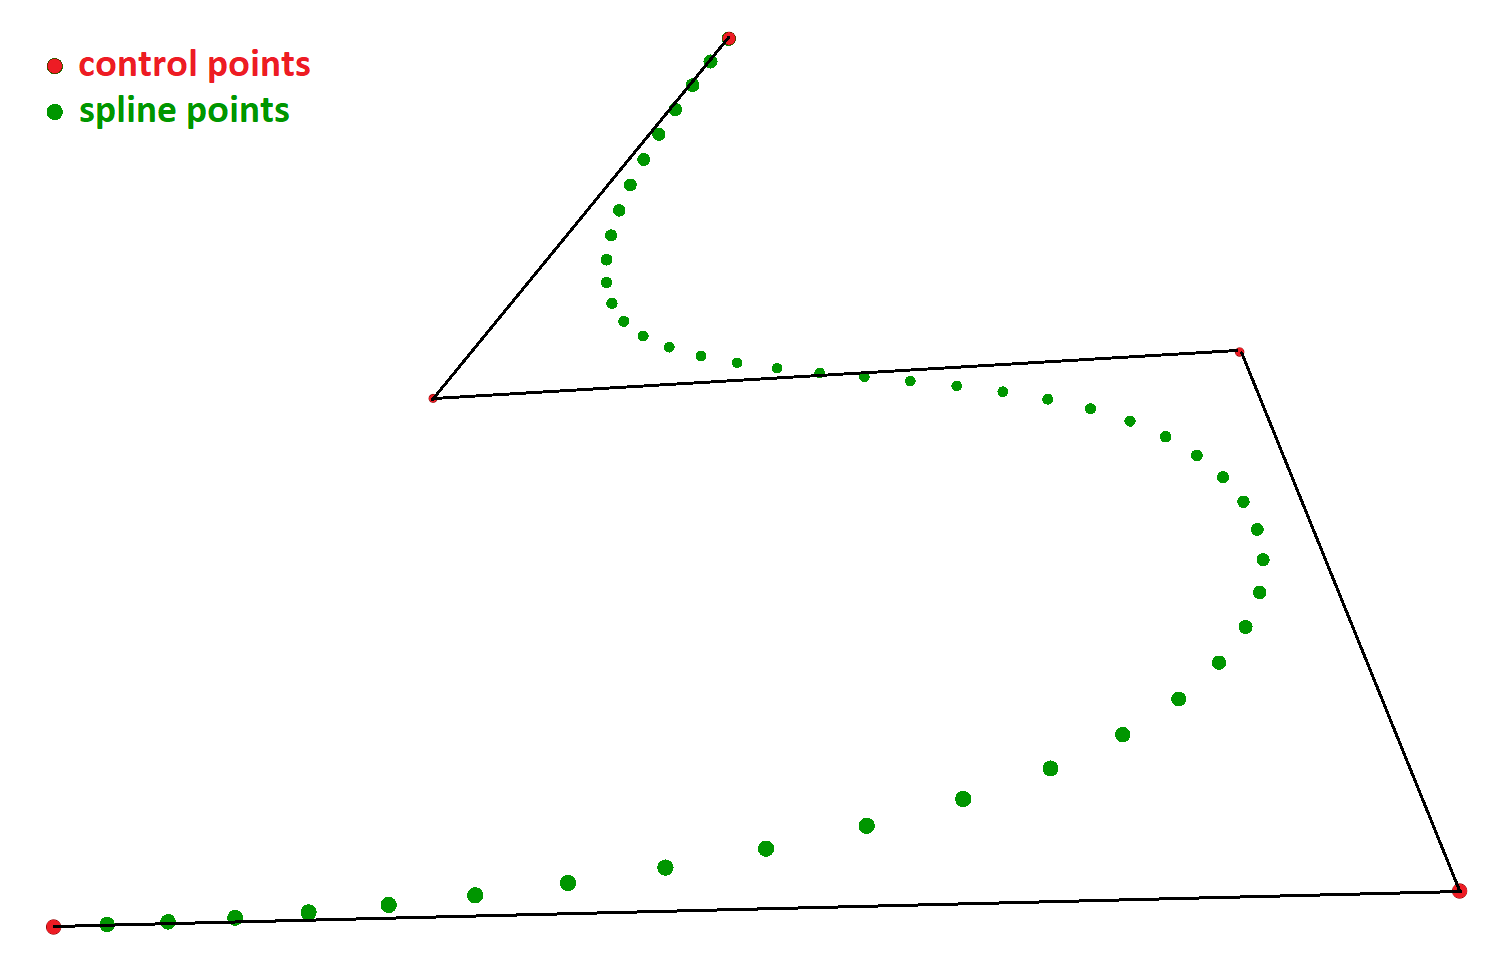
\includegraphics[width=\textwidth]{splinecurve}
\caption{Spline curve with 1D parameter}
\label{splinecurve}
\end{subfigure}
\begin{subfigure}[b]{0.48\textwidth}
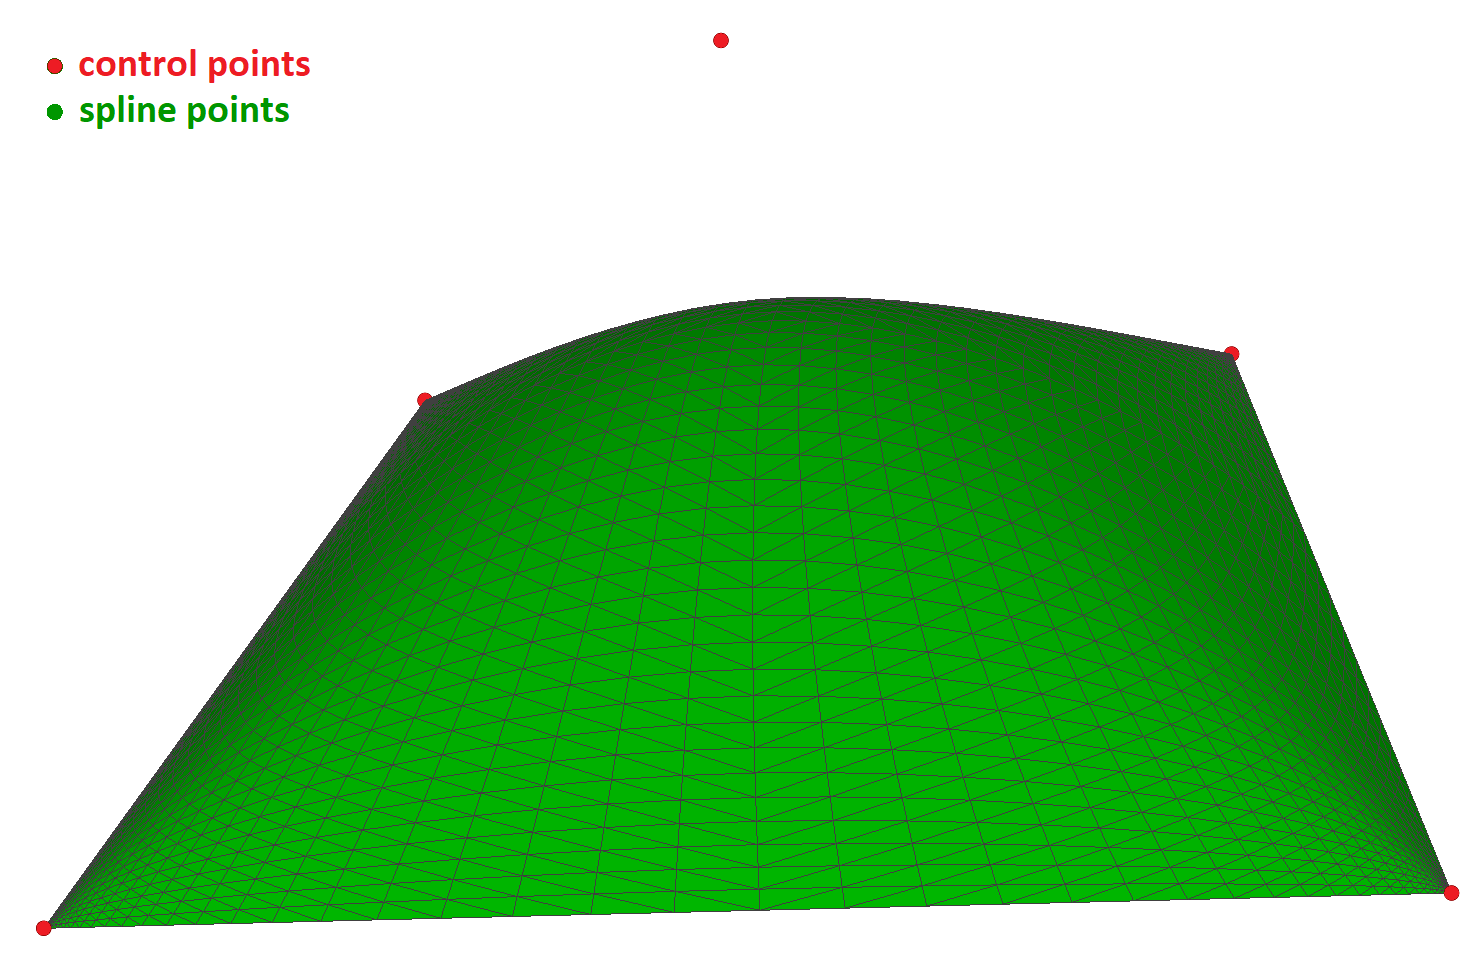
\includegraphics[width=\textwidth]{splinesurface}
\caption{Spline surface with 2D parameter}
\label{splinesurface}
\end{subfigure}
\caption{Spline curve and surface consisting the same 5 control points with one- and two-dimensional parametrisation, respectively.}
\end{figure}

Dragging the control points shifts a restricted part of the surface towards it. How the area of effect (\emph{AOE}) looks lies in the knots and their distance from each other. Knots are less intuitive to understand, since control points exist in the 3D real space, meanwhile knots exist in the parametric space that is "invisible". This will be explained in more detail later in Section \ref{sec:tech}.

\vspace{6pt}

The goal of this essay is to give some intuition about how such surfaces change by altering the parametric space, in restriction of T-spline surfaces which have exceptionally high flexibility in terms of knots.

\vspace{12pt}

\begin{large}
\section{Technical background}
\label{sec:tech}
\end{large}

\vspace{12pt}

In order to get a full picture on T-splines, it is best to start with B-splines. Depending on the dimension, one can talk about a spline curve or a spline surface. The fundamental mathematics work similarly, though. Either way, the equation that describes a spline is a parametric equation where the substituted values exist in the parametric space that have nothing to do with the real 3D space. For nice surfaces, however, a loose connection is made between them two, but mathematically speaking, they are separate. That is why it is not intuitive how certain changes in the parametric space alter the real space.

\subsection{B-spline}

\vspace{6pt}
Spline is a generic term. There are several different types, but the base of 3D modelling relies on B-splines. For all those mathematics-oriented readers out there, what it means from a more technical perspective can be found in Gallier (2018). What is important to know is that the B-spline equation is a recursive function defined by Equation (\ref{bspline_rec}) (\emph{B-spline}, 2022).

\begin{equation}
\begin{split}
B_{i,k}(p) & = m_{i,k-1}(p) B_{i,k-1}(p) + \big(1 - m_{i+1,k-1}(p)\big) B_{i+1,k-1}(p), \\
& \text{where} \\
m_{i,k}(p) & =
    \begin{cases}
      \frac{p-t_i}{t_{i+k}-t_i}, & t_{i+k} \neq t_i \\
      0, & \text{otherwise}
    \end{cases}
\\
B_{i,0}(p) & =
    \begin{cases}
      1, & t_{i+k} \leq p < t_{i+1} \\
      0, & \text{otherwise}
    \end{cases}
\end{split}
\label{bspline_rec}
\end{equation}

$B_{i,k}$ is called B-spline basis function of degree $k$, where $i$ goes from 0 to the number of knots. $t_i$ is the (parametric) coordinate of the $i$th knot, and $p$ denotes the parameter, the variable of a spline equation.

Each recursion of this function is a separated function on its own, but they only have nonzero values between certain knots. Therefore one can look at knots as limits, thresholds between two basis functions.

Let us look at now some basis functions in Figure \ref{basisfunctions} to understand knots better. A basis function of degree 0 is a simple indicator function that is 1 between two consecutive knots and 0 elsewhere. These two knots are defined by the first index of the basis function. $B_{0,0}$ is nonzero between the first and second knot, $B_{1,0}$ is nonzero between the second and third knot, and so on and so on. $B_{3,0}$ - that is shown in Figure \ref{basisfunctions} - is nonzero between the fourth and fifth knot. The degree of a basis function signals the spanning of the nonzero interval. Degree 0 spans across two adjacent knots, i.e. one "knot distance". Degree 1 spans across three adjacent knots, i.e. two "knot distance", meanwhile degree 3 does over five knots - as also shown in Figure \ref{basisfunctions}. The higher the degree, the smoother the basis function is.

\begin{figure}[H]
\centering
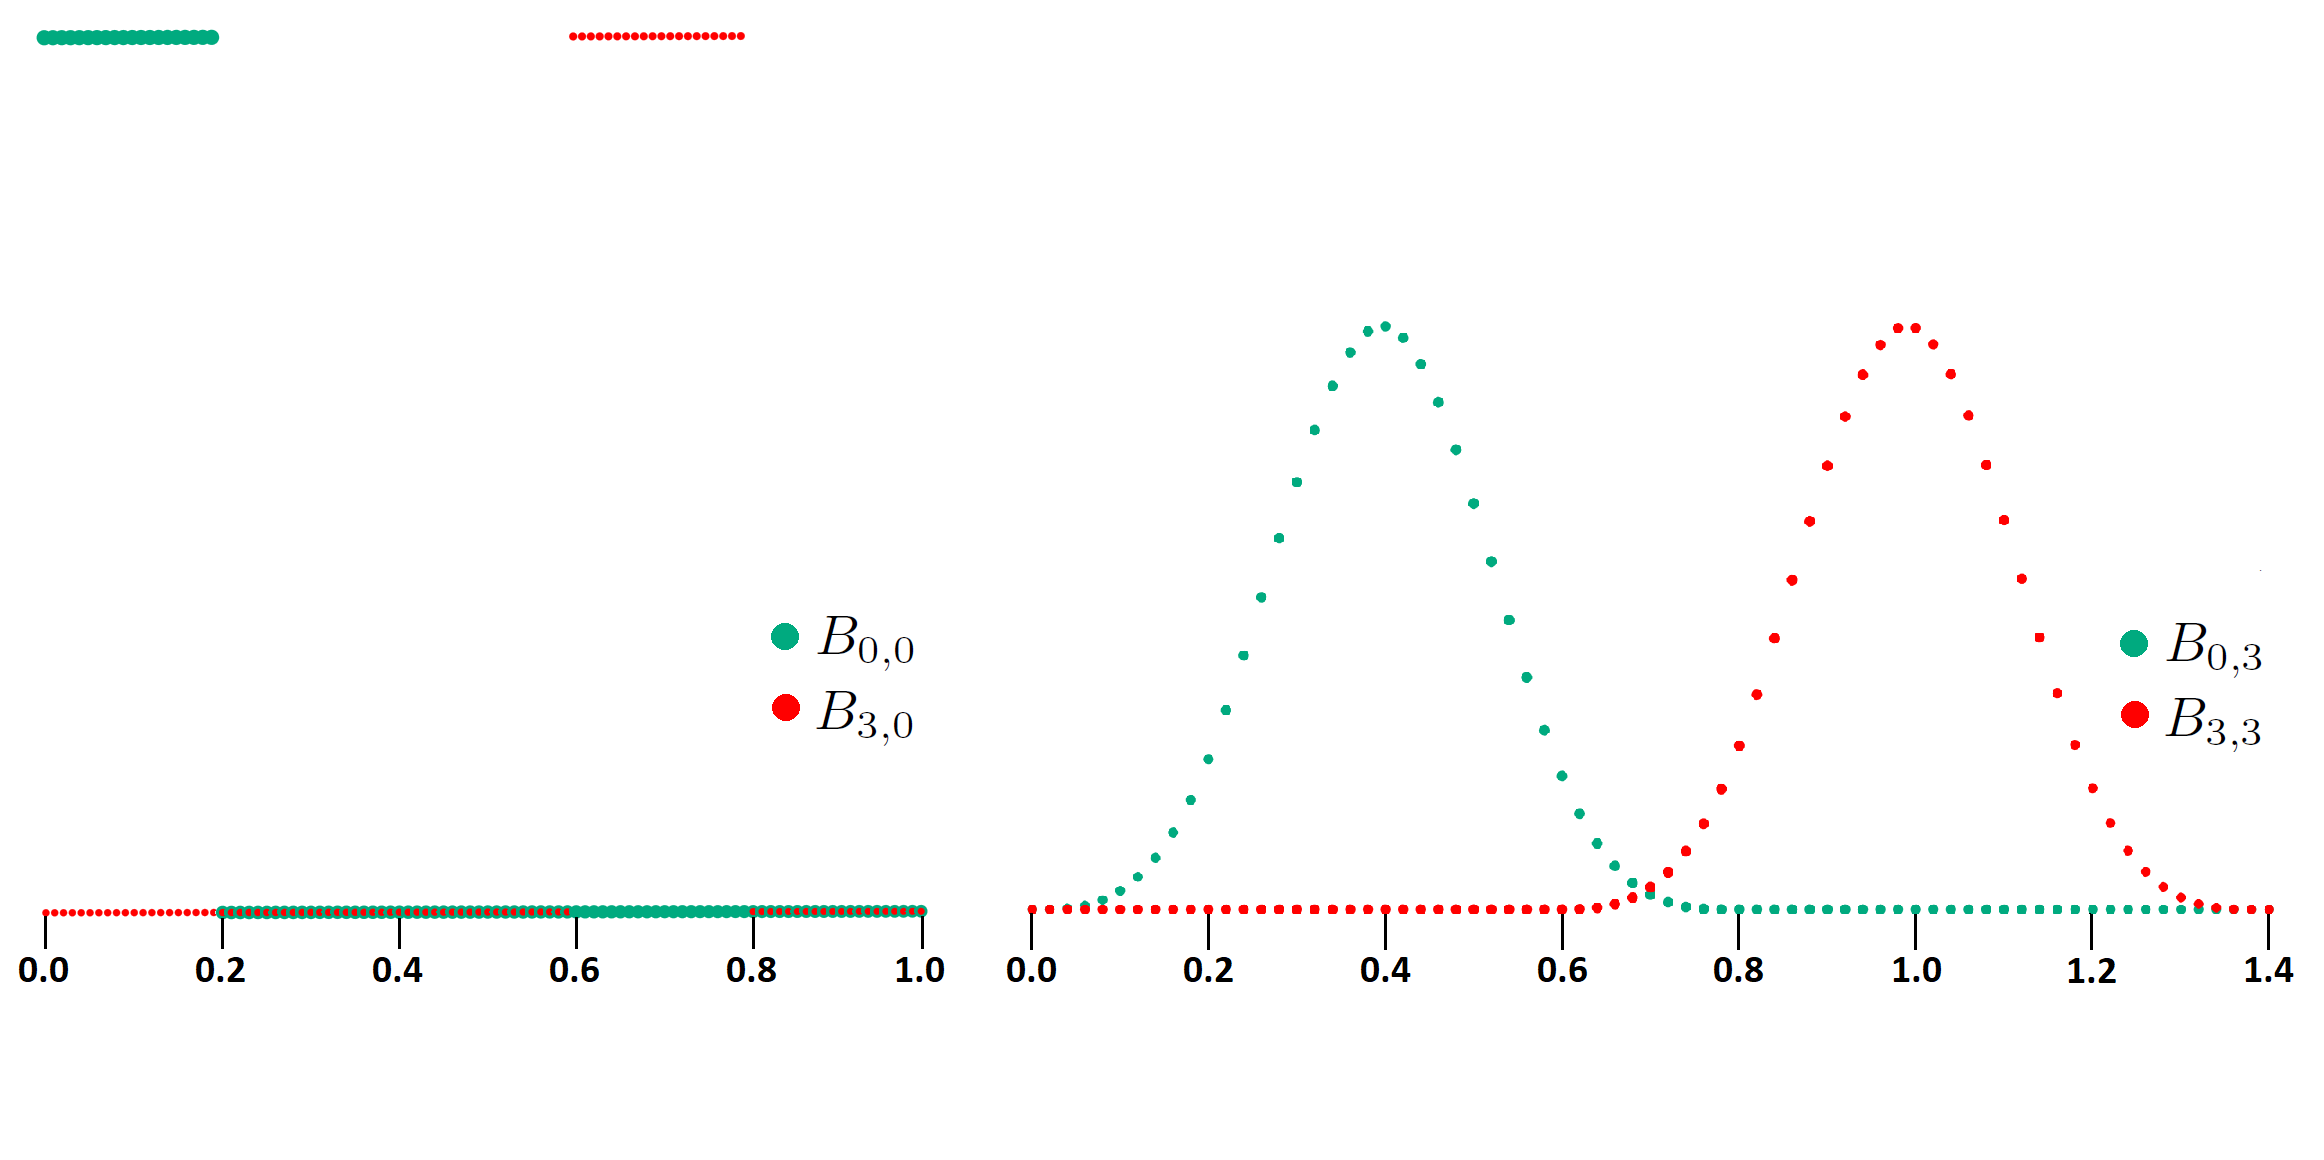
\includegraphics[width=\textwidth]{basisfunctions}
\caption{Two-two basis functions of degree 0 and 3, respectively. Indicated points on horizontal line represent the defined knots for these basis functions.}
\label{basisfunctions}
\end{figure}

$B_{i,3}$ is more complicated to understand why it looks the way it does. Just by looking at Equation (\ref{bspline_rec}) it is not clear, since the recursion is already on a higher level. $B_{i,3}$ consist of several previous $B_{i, k}$. An illustrative explanation can be found on \emph{B-spline basis functions} (2001)\footnote{Further illustration and explanation can be found on \emph{B-spline curve} (2009)}.

Although the code will not crash, mathematically speaking knots are supposed to follow each other on a nondecreasing order in a \emph{knot vector} (\emph{B-splines}, n.d.). A knot vector contains knots that can be arbitrary, but meaningful knots do exist, and they are advised to be used. What is considered meaningful is up to the individual, the situation, and circumstances. For easier programming\footnote{and for numerical accuracy}, knot vector is represented between 0 and 1(\emph{B-spline curve}, 2009) for all upcoming examples\footnote{except Figure \ref{basisfunctions}}.

Depending on the differences of adjacent knots, \emph{uniform, open uniform, and non-uniform} knot vectors are distinguished. The difference in a uniform knot vector is constant, in a non-uniform knot vector it is arbitrary. An open uniform knot vector is similar to a uniform one, but the first and last \emph{k} knots (where $k$ = degree) are equal (\emph{B-splines}, n.d.) (\emph{B-spline basis functions}, 2001).

\subsection{B-spline curve}

\vspace{6pt}
A B-spline is curve is technically a combination of the aforementioned B-spline basis functions that is defined by control points, knots, and degree. Its function is shown in Equation (\ref{func:bsplinecurve})\footnote{Assuming each control point has weight = 1}.

\begin{equation}
C_{k, \mathbf{t}}(p) = \sum_{i}^n R_{i} B_{i, k}(p),
\label{func:bsplinecurve}
\end{equation}

where $k$ represents the degree, \emph{\textbf{t}} is the knot vector, $R_i$ is the $i$th control point's 3D coordinate, and $n$ is total number of control points.

If the reader is familiar with Fourier or Taylor series, fundamentally they are similar to a B-spline curve equation. In comparison, the basis functions have the role of cosines and sines from Fourier series. They serve the \emph{basis} which have to be multiplied by some "weight"\footnote{The "weight" here refers to the control point.}. In a way, a B-spline curve equation is a series of B-splines; in other words, an expansion, but unlike Fourier or Taylor series, the sum is never infinite.

Equation (\ref{func:bsplinecurve}) suggests that the order of the control points on a curve affects the end result. Figure \ref{bsplinecurvecomparsion} supports that the shape of a B-spline curve is indeed different with swapped control points.

\begin{figure}[H]
\centering
\begin{subfigure}[b]{0.48\textwidth}
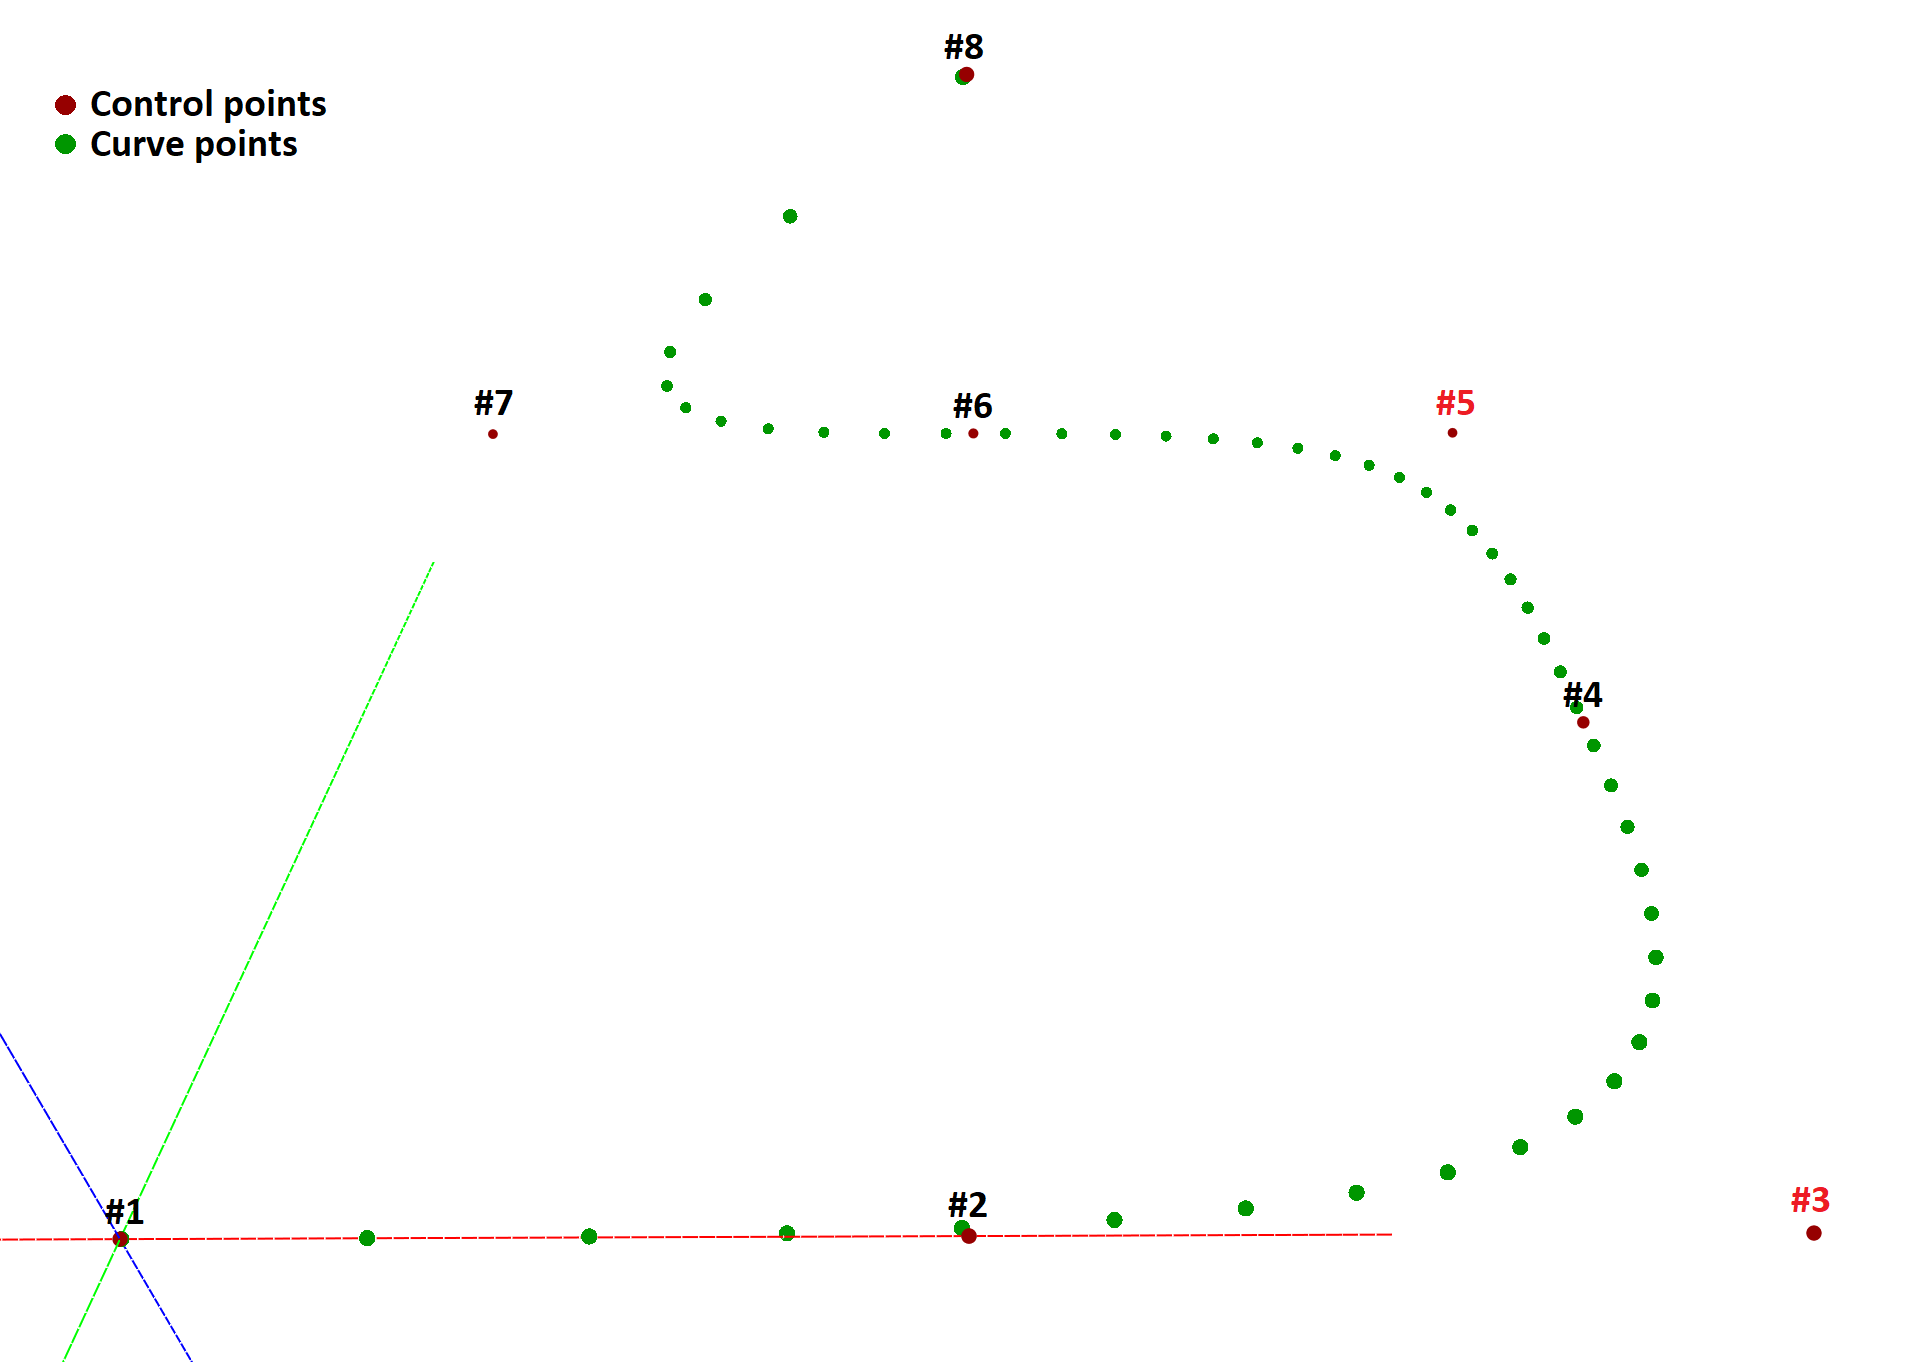
\includegraphics[width=\textwidth]{bsplinecurve1}
\caption{}
\label{bsplincecurve1}
\end{subfigure}
\begin{subfigure}[b]{0.48\textwidth}
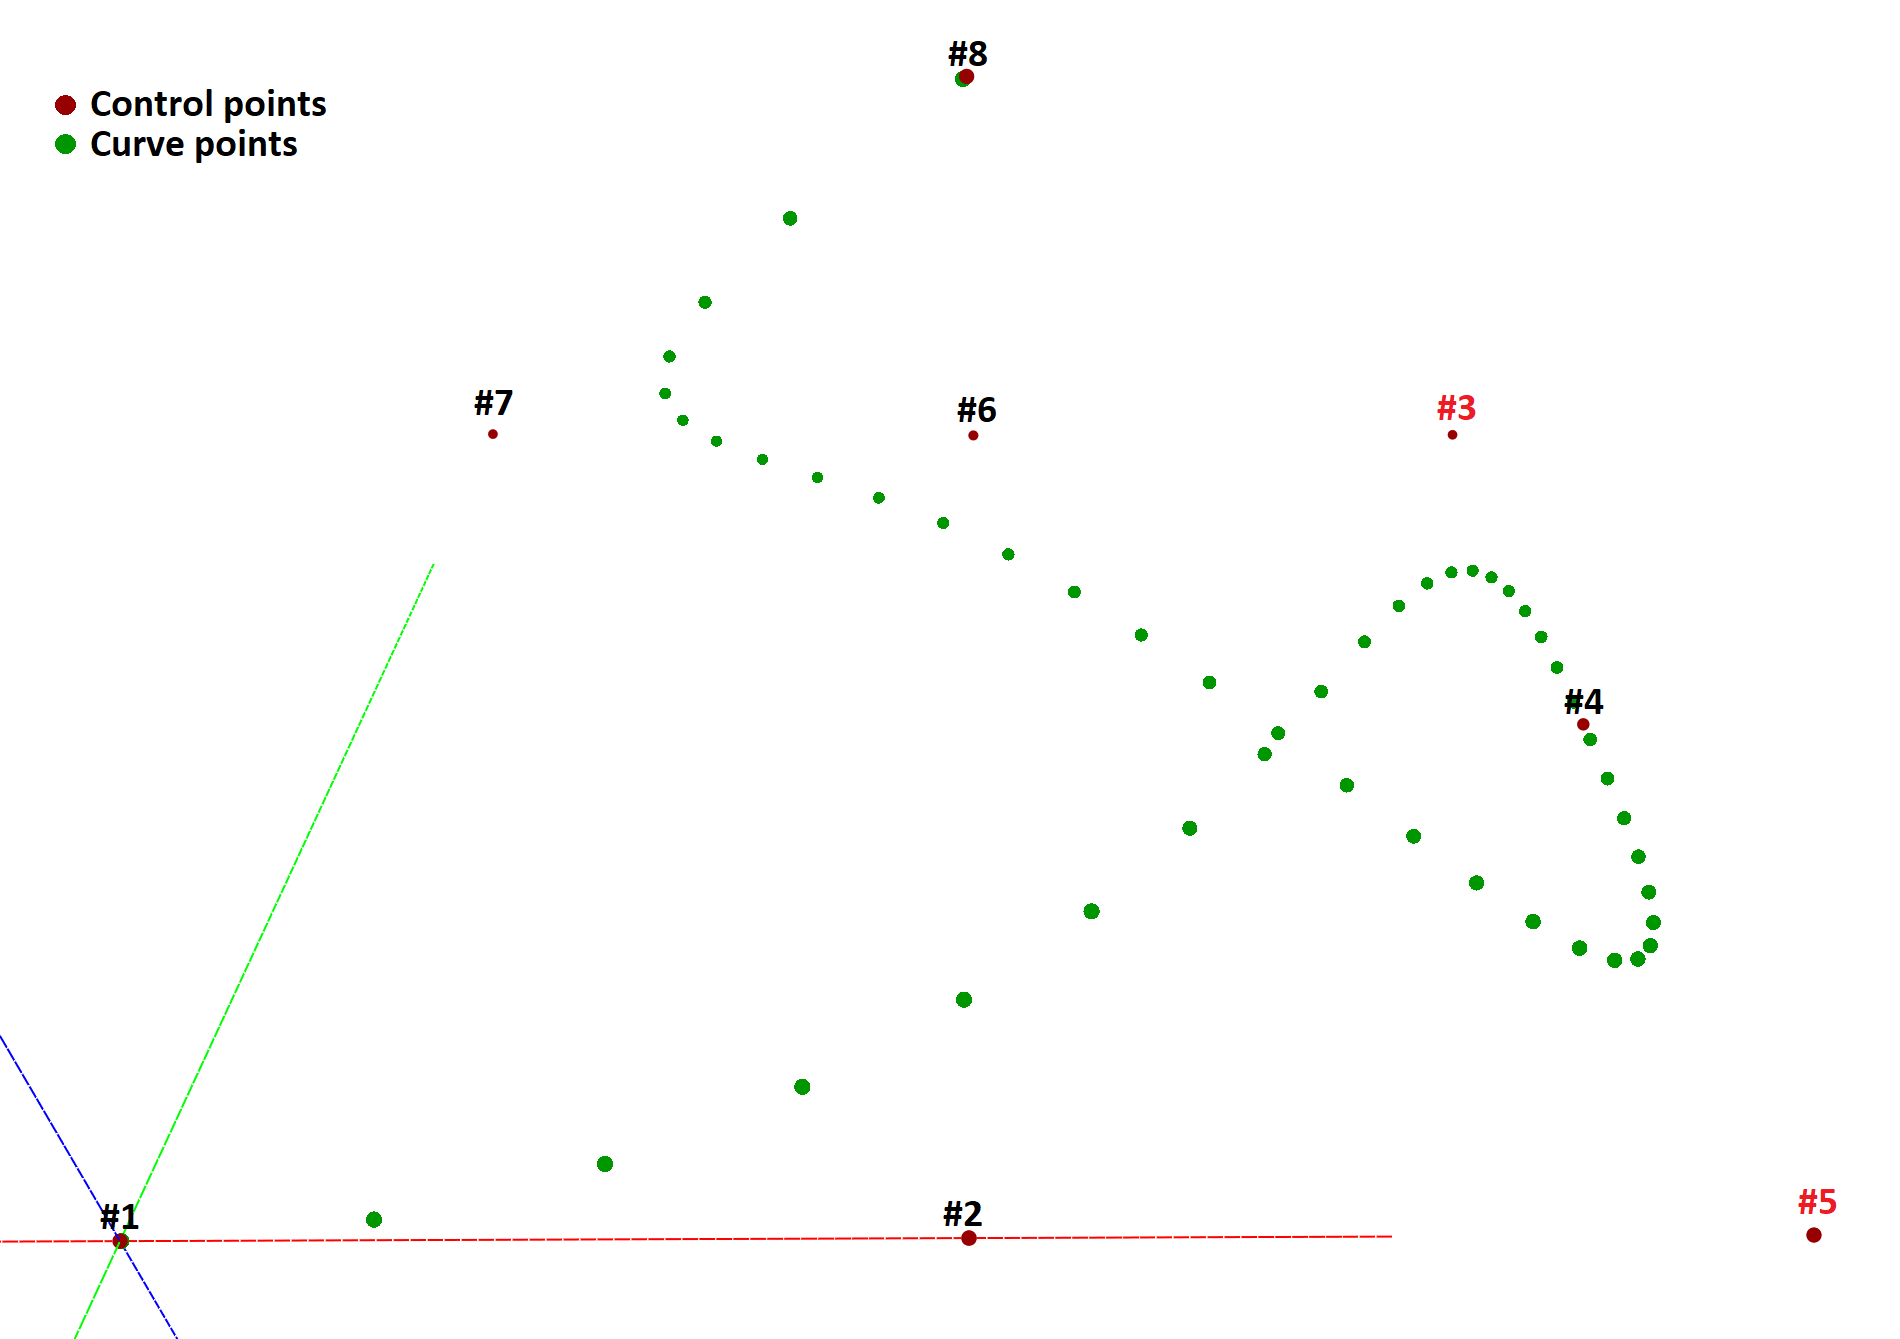
\includegraphics[width=\textwidth]{bsplinecurve2}
\caption{}
\label{bsplincecurve2}
\end{subfigure}
\caption{B-spline curves with the same eight control points with different order in function of degree 3.}
\label{bsplinecurvecomparsion}
\end{figure}

If a control point is in third place, $B_{2,k}$ is used, and in fifth place $B_{4,k}$ is associated with it. That means that different knots have impact on the control points, so the third and fifth control points' spanning areas are switched.

\subsubsection{Knot vector}

\vspace{6pt}

When a B-spline curve is defined, a knot vector is also initialised with it. Depending on the type of knot vector, there are three categories of a B-spline curve: \emph{open, clamped}, and \emph{closed} (Ching-Kuang, n.d.). Open and closed B-splines will be omitted in this essay, only clamped curves will be discussed. However, even clamped curves are open in the general sense - such as shown in Figure \ref{curvetypes}.

\begin{figure}[H]
\centering
\begin{subfigure}[b]{0.32\textwidth}
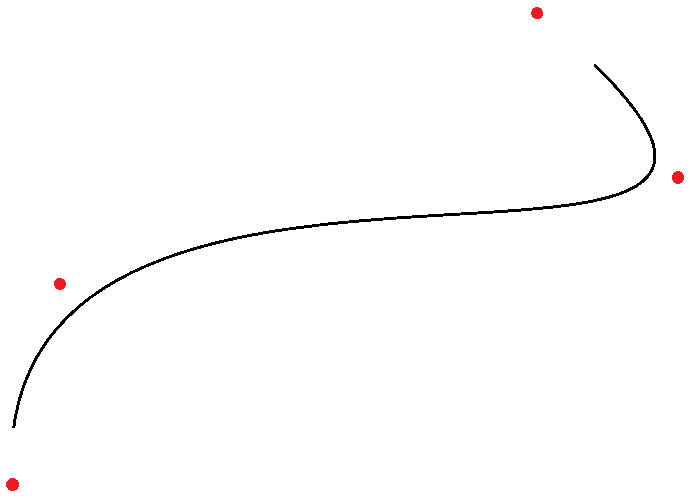
\includegraphics[width=\textwidth]{open}
\caption{Open curve.}
\label{open}
\end{subfigure}
\begin{subfigure}[b]{0.32\textwidth}
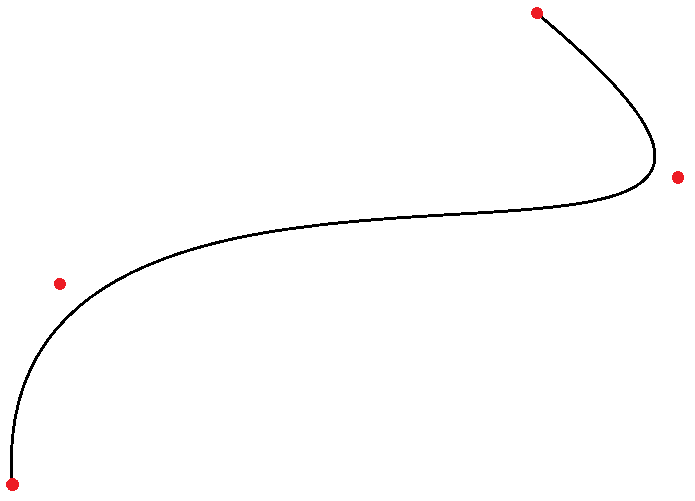
\includegraphics[width=\textwidth]{clamped}
\caption{Clamped curve.}
\label{clamped}
\end{subfigure}
\begin{subfigure}[b]{0.32\textwidth}
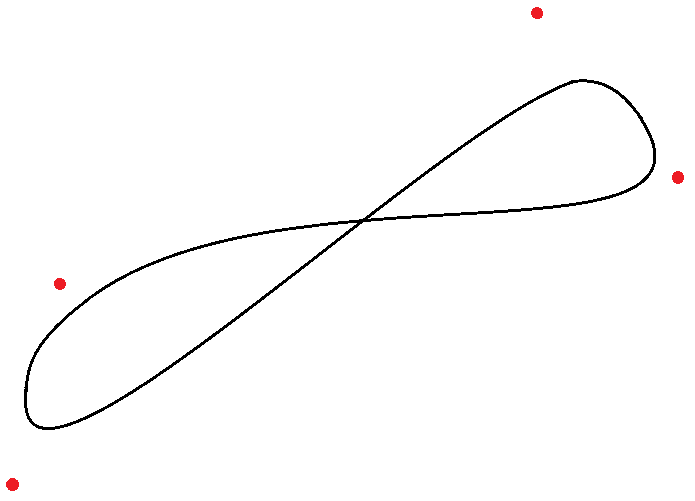
\includegraphics[width=\textwidth]{closed}
\caption{Closed curve.}
\label{closed}
\end{subfigure}
\caption{Different B-spline curve types.}
\label{curvetypes}
\end{figure}

Clamped curve is probably the most intuitive among the three. It starts and ends in a control point, and unless those two controls points are the same, the curve does not circle back to the initial point. Those two control points serve as a sort of guide, so it is easier to imagine the result of a curve even without seeing it.

\vspace{6pt}
Now let us assume that the associated knot vector is open uniform, and has a range of [0,1]. If degree = 3 then this looks like (\ref{openuniformknotvector}).

\begin{equation}
\mathbf{t} = (0, 0, 0, 0, 0.2, 0.4, 0.6, 0.8, 1, 1, 1, 1)
\label{openuniformknotvector}
\end{equation}

The more control points are introduced, the more knots are required. In this specific example in (\ref{openuniformknotvector}), there are eight control points - similarly to Figure \ref{bsplinecurvecomparsion}. In case of $k$ = 3 degree, there are $k+1$ 0s, $k+1$ 1s, and $n-(k+1)$ intermediate equidistant knots (\emph{B-splines}, n.d.). That means that $n$ $\geq$ k+1 always.

Let us look at this from the control points' point of view. With $k$ = 3, basis functions span across five knots. The first control point therefore also spans across five knots, namely, the first five.

\begin{equation}
\mathbf{t}_1 = (0, 0, 0, 0, 0.2) \longleftrightarrow R_1
\end{equation}

That means that the first control point has an impact on the shape until the first nonnull knot. When a parameter $\geq$ 0.2 is substituted, $B_{1,3}$ will be 0, so $R_1$ will not affect the curve.
Simply, when the order of control points is set in case of a B-spline curve, the appropriate knots are also designated.

\subsection{B-spline surface}

\vspace{6pt}
B-spline surfaces are very similar to B-spline curves, but their parameter is two dimensional.

\begin{equation}
S_{k,\mathbf{t}}(p_1, p_2) = \sum_{i}^n\sum_{j}^m B_{i,k}(p_1)B_{j,l}(p_2) R_{i,j}
\label{func:bsplinesurface}
\end{equation}

In Equation (\ref{func:bsplinesurface}) (\emph{B-spline}, 2022) weight is omitted again, so all control points have weight = 1. In this essay, $l$= $k$, but mathematically speaking it is not necessarily. This decision was purely arbitrary to simplify the mathematics without losing much generalisation. It also makes sense to have basis functions of same degree in both parametric dimensions.

Let us look at an example that is shown in Figure \ref{bsplinesurfacecomparsion}.

\begin{figure}[H]
\centering
\begin{subfigure}[b]{0.48\textwidth}
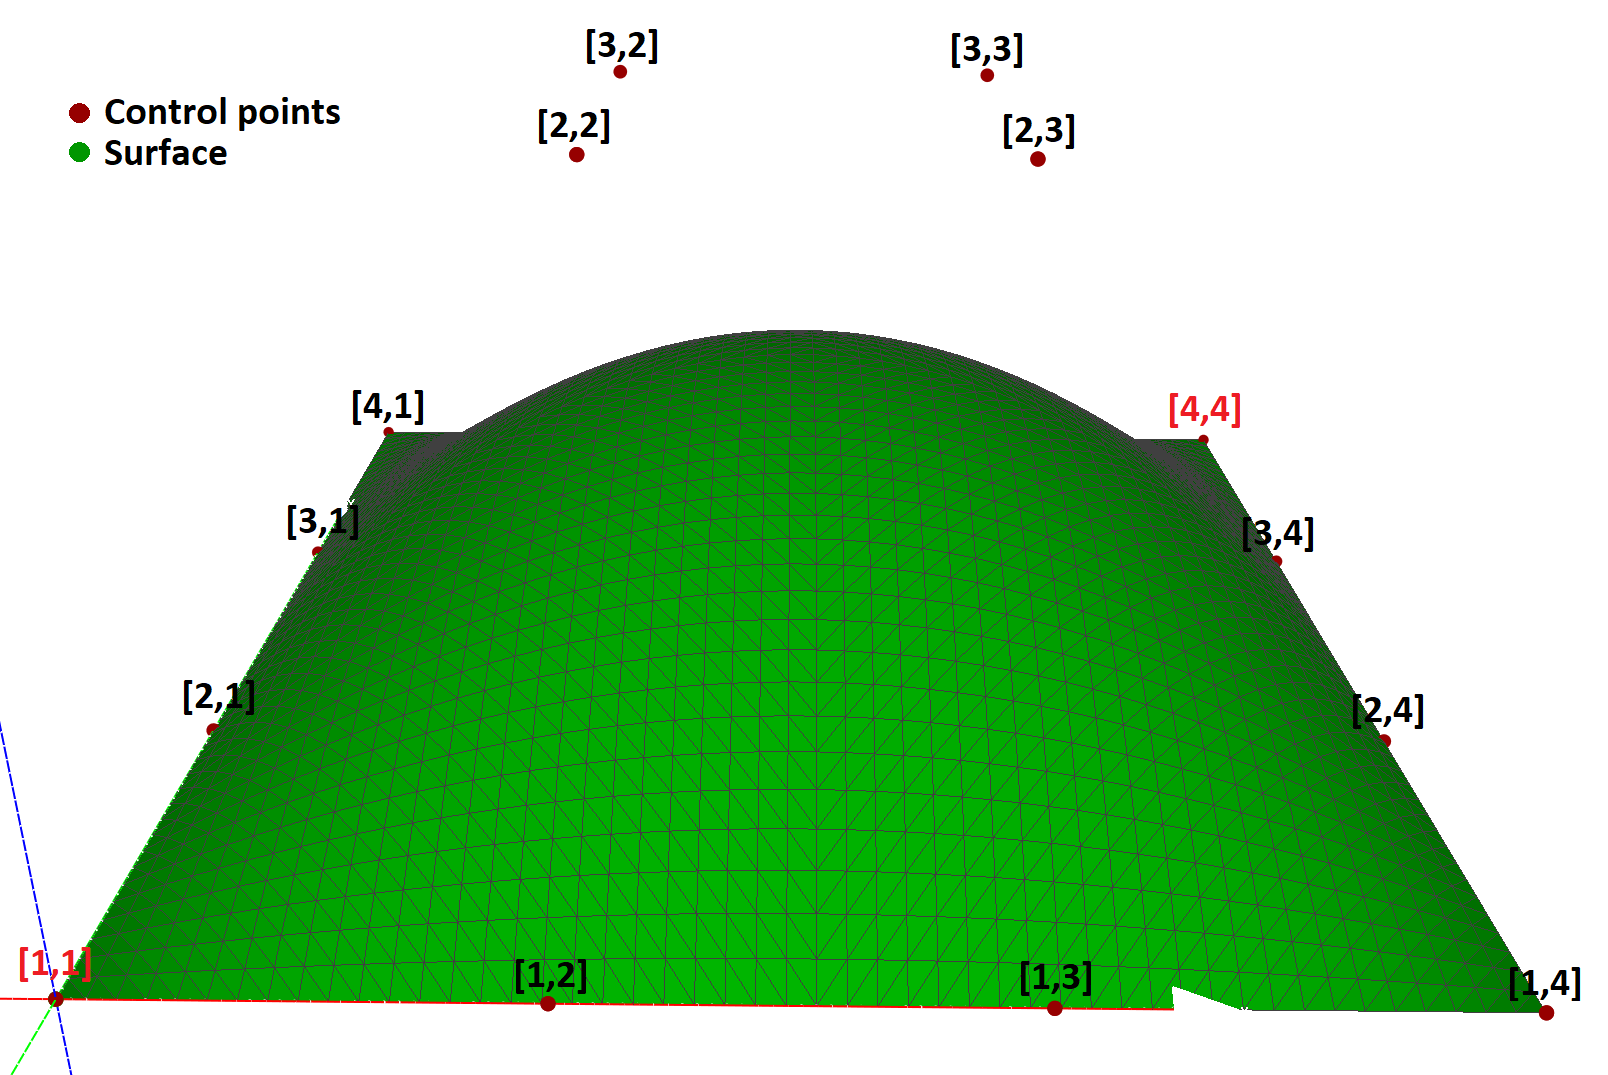
\includegraphics[width=\textwidth]{bsplinesurface1}
\caption{}
\label{bsplinesurface2}
\end{subfigure}
\begin{subfigure}[b]{0.48\textwidth}
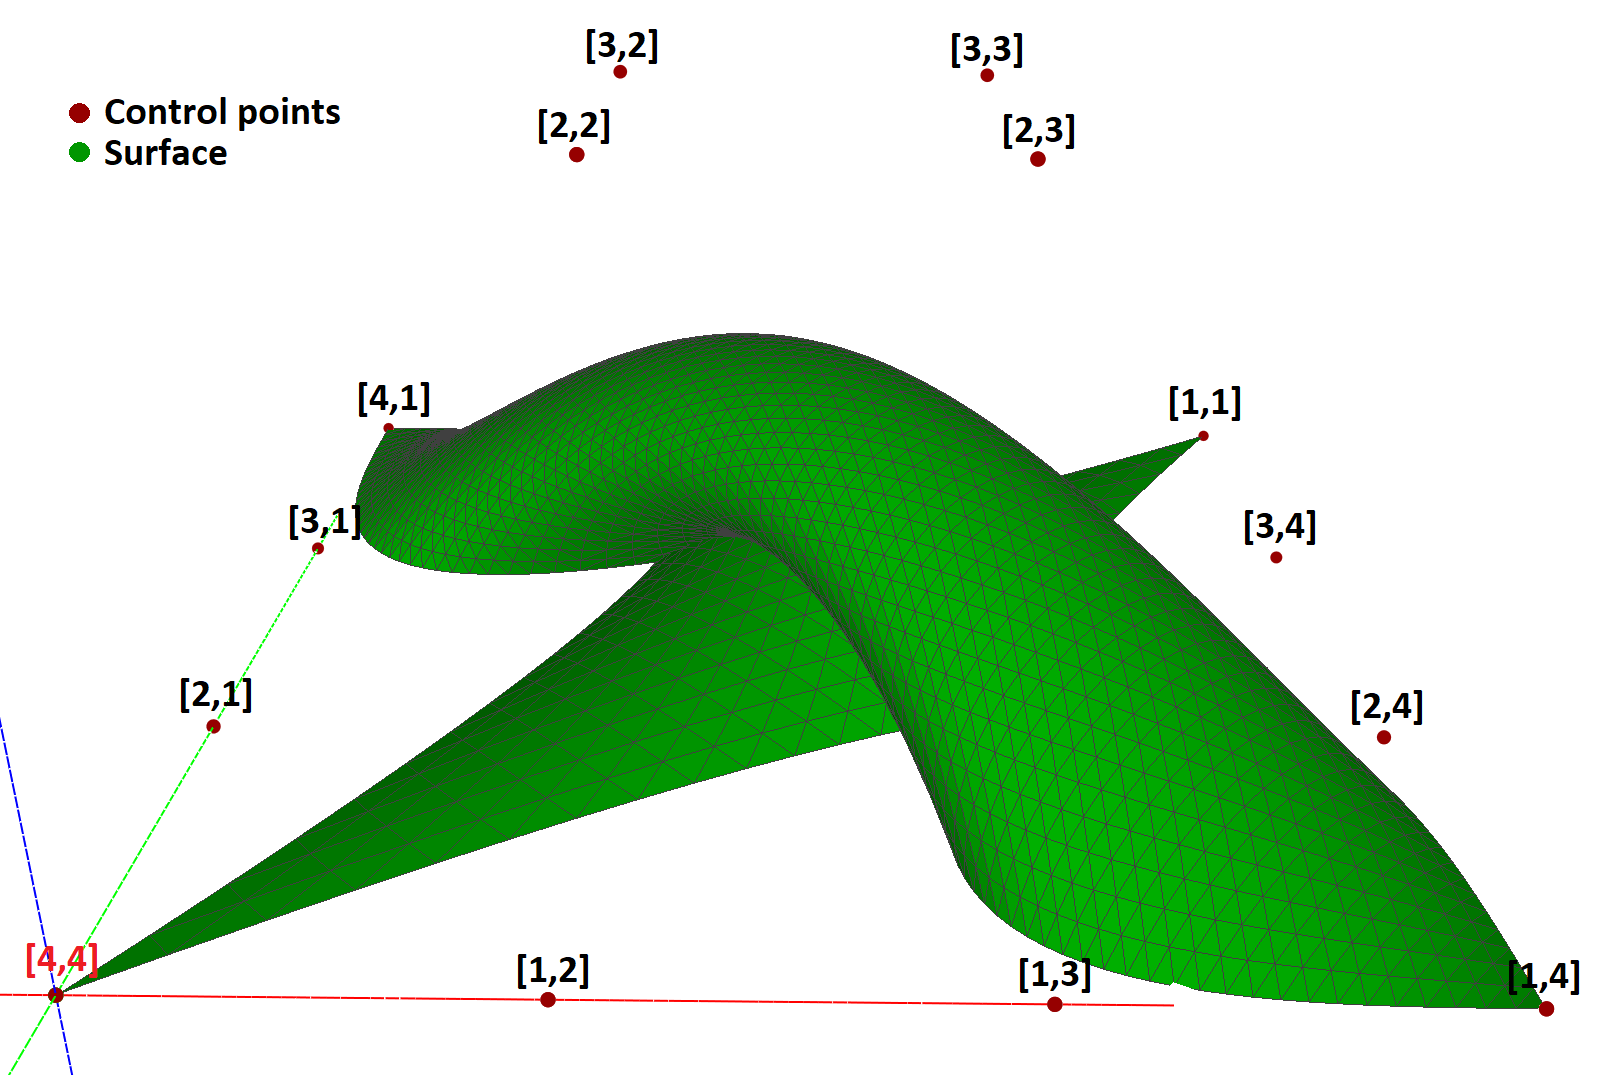
\includegraphics[width=\textwidth]{bsplinesurface2}
\caption{}
\label{bsplinesurface2}
\end{subfigure}
\caption{B-spline surfaces with the same 16 control points with different order in function of degree 3. $R_{4,2}$ and $R_{4,3}$ are not visible because they are in the back covered by the surface.}
\label{bsplinesurfacecomparsion}
\end{figure}

Both surfaces are defined by the same 16 control points, but $R_{1,1}$ and $R_{4,4}$ are swapped, so the order of control points has changed, and with that, the surface has changed, as well. Similarly to a B-spline curve, there is a part on the surface that stayed intact, because not the entire surface is affected by these two control points.

The order in case of a surface is also two dimensional, so instead of a control point vector, a control point matrix is defined - as it is shown in Equation (\ref{func:bsplinesurface}) with a double indexed $R_{ij}$. There are 16 control points and they have been put into a 4 $\times$ 4 control point matrix.

\subsubsection{Knot vectors}

\vspace{6pt}
Since a surface is two dimensional\footnote{embedded in 3D}, there are two knot vectors associated with a B-spline surface. The number of knots are defined by the degree and number of control points in each direction. This surface contains 4 control points in both direction - hence the 4 $\times$ 4 = 16 points -, and its degree is 3. Therefore the corresponding knot vectors are both as in Equation (\ref{surfaceknots}).

\begin{equation}
\mathbf{t} = (0, 0, 0, 0, 1, 1, 1, 1)
\label{surfaceknots}
\end{equation}

\subsection{T-spline}

\vspace{6pt}

The fundamental difference between T-spline and B-spline lies in \emph{freedom}. While in a B-spline surface a rigid grid of control points in the right order with their respective knot vectors defines the area, in T-spline it is much more flexible than that. It can, however, describe the same surface with the right settings as shown in Figure \ref{surfacegrids}.

\begin{figure}[H]
\centering
\begin{subfigure}[b]{0.48\textwidth}
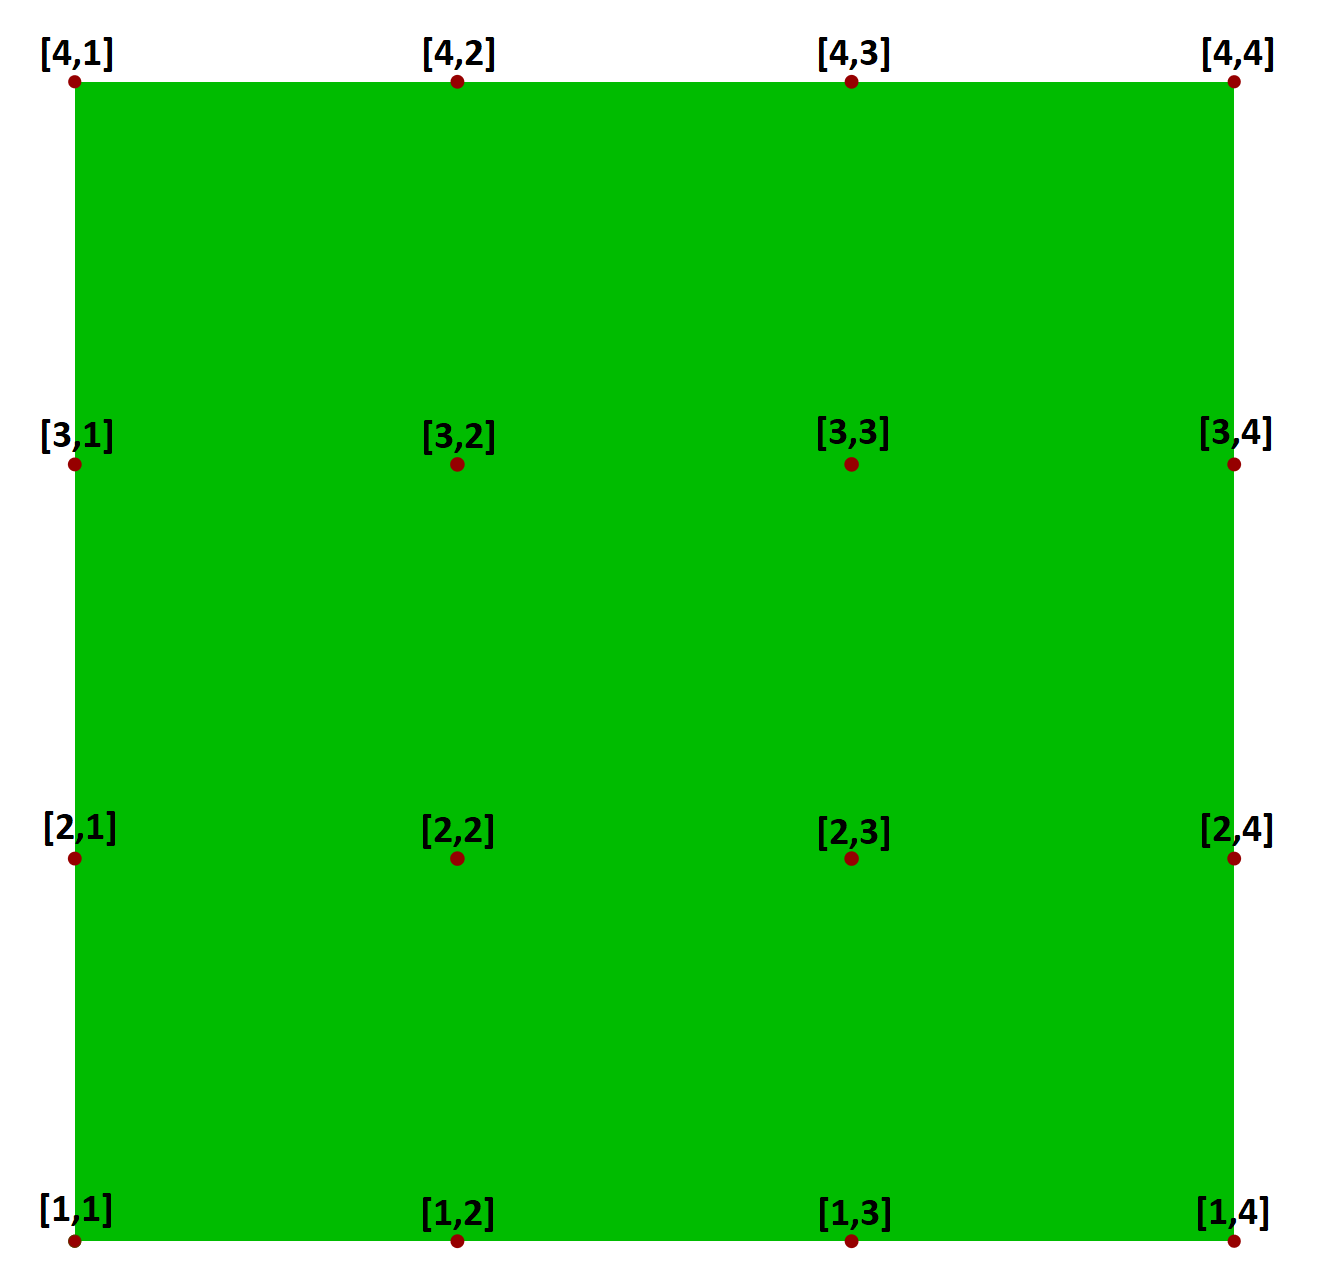
\includegraphics[width=\textwidth]{splinegrid1}
\caption{B-spline surface with 16 control points.}
\label{splinegrid2}
\end{subfigure}
\begin{subfigure}[b]{0.48\textwidth}
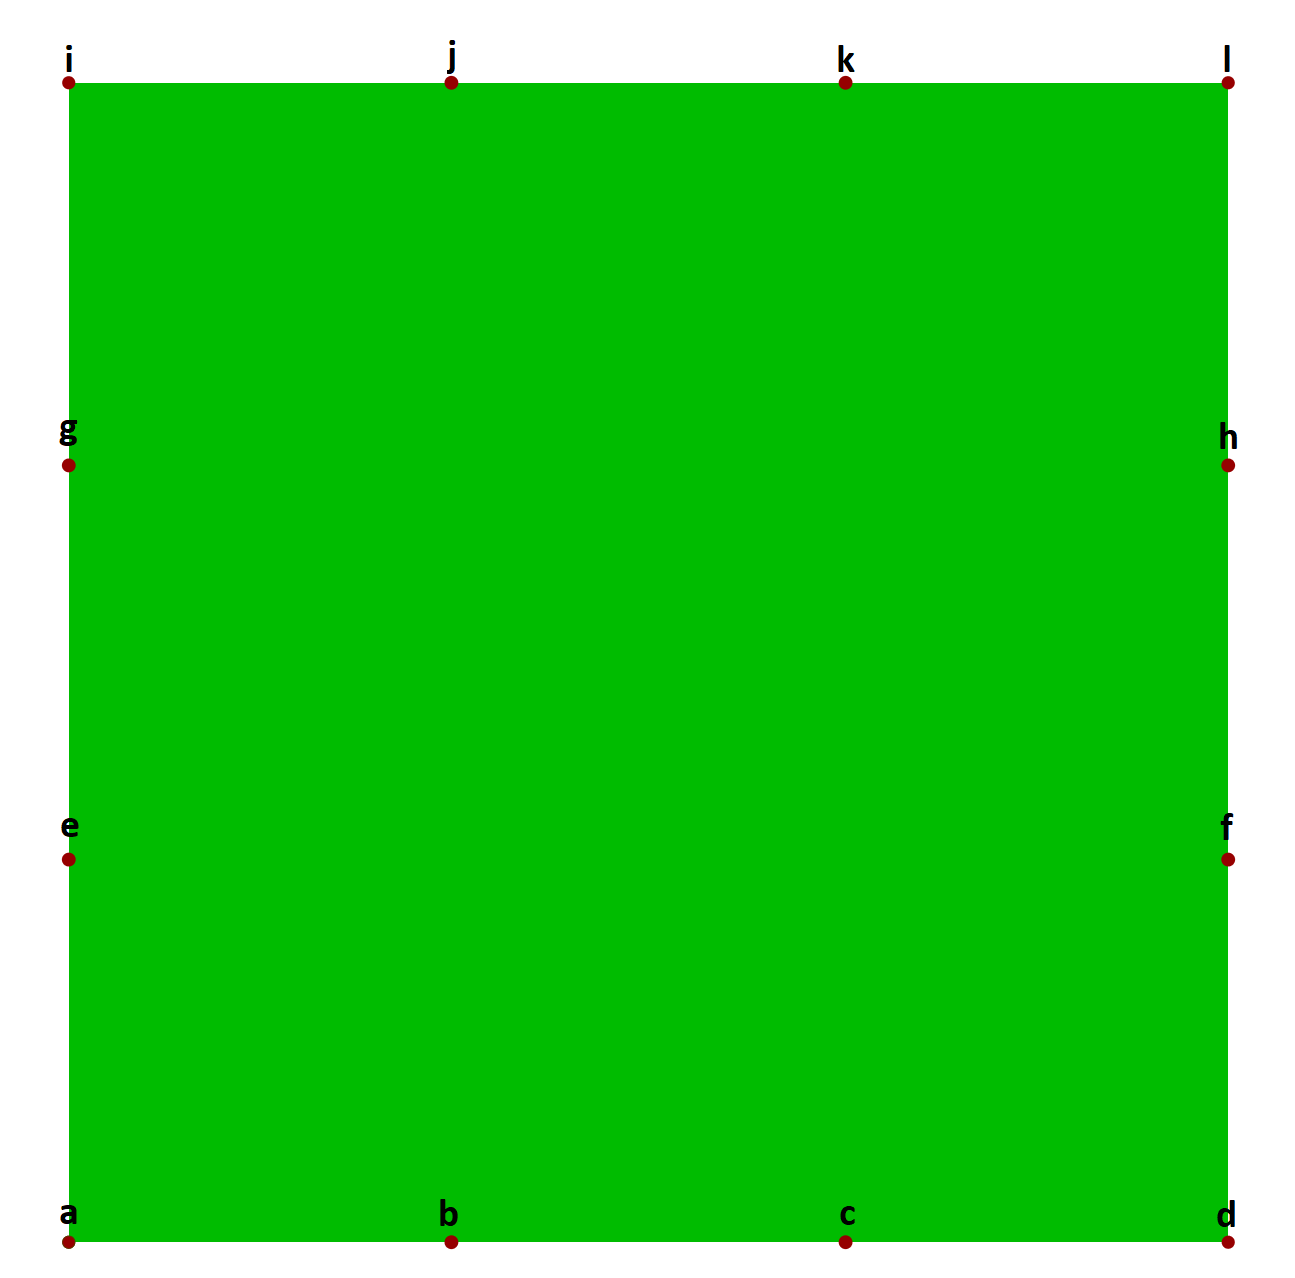
\includegraphics[width=\textwidth]{splinegrid2}
\caption{T-spline surface with 12 control points.}
\label{splinegrid2}
\end{subfigure}
\caption{The same surface described by B-spline and T-spline equations.}
\label{surfacegrids}
\end{figure}

T-spline surfaces use B-spline basis functions as well, but they are all $B_{0, 3}$ with different knot vectors.

\begin{equation}
T(p_1, p_2) = \sum_i^n B_{0,3,\mathbf{t_{i1}}}(p_1)B_{0,3,\mathbf{t_{i2}}}(p_2) R_{i},
\label{eq:tspline}
\end{equation}

where $\emph{\textbf{t}}_{i1}$ and $\emph{\textbf{t}}_{i2}$ indicate the corresponding knots in both directions (Sederberg et al., 2004). These knots are associated to one-one $R_i$ control point. Since $B_{0,3}$ is a basis function of degree 3, $\emph{\textbf{t}}_{i1}$ and $\emph{\textbf{t}}_{i2}$ are 5-long knot vectors. It is also worth mentioning, that since the basis functions do not depend on $i$ directly (only through the knot vectors of control points), the order of the control points do not matter. The basis functions are connected to the control point itself and not its place in a sequence of points.

\vspace{6pt}
In case of B-spline, the order of control points dictates which knots are associated with certain control points. Here, each control point is separately associated with its knots. A B-spline knot vector is a set of knots designated to define a sequence of subsets of knots, and the order of control points decides which control point receives which subset. Since a T-spline control point has its own "subset"\footnote{It has its own knot vector.}, there is no need for a specific order. That is why in Figure \ref{splinegrid2} each control point was denoted with a letter and not a number, to indicate its orderless nature.

\subsubsection{Knot vector}

\vspace{6pt}
The power of T-spline comes from the individual adjustability of knot vectors. That is clearly illustrated in Figure \ref{tsplineexs}.

\begin{figure}[H]
\centering
\begin{subfigure}[b]{0.48\textwidth}
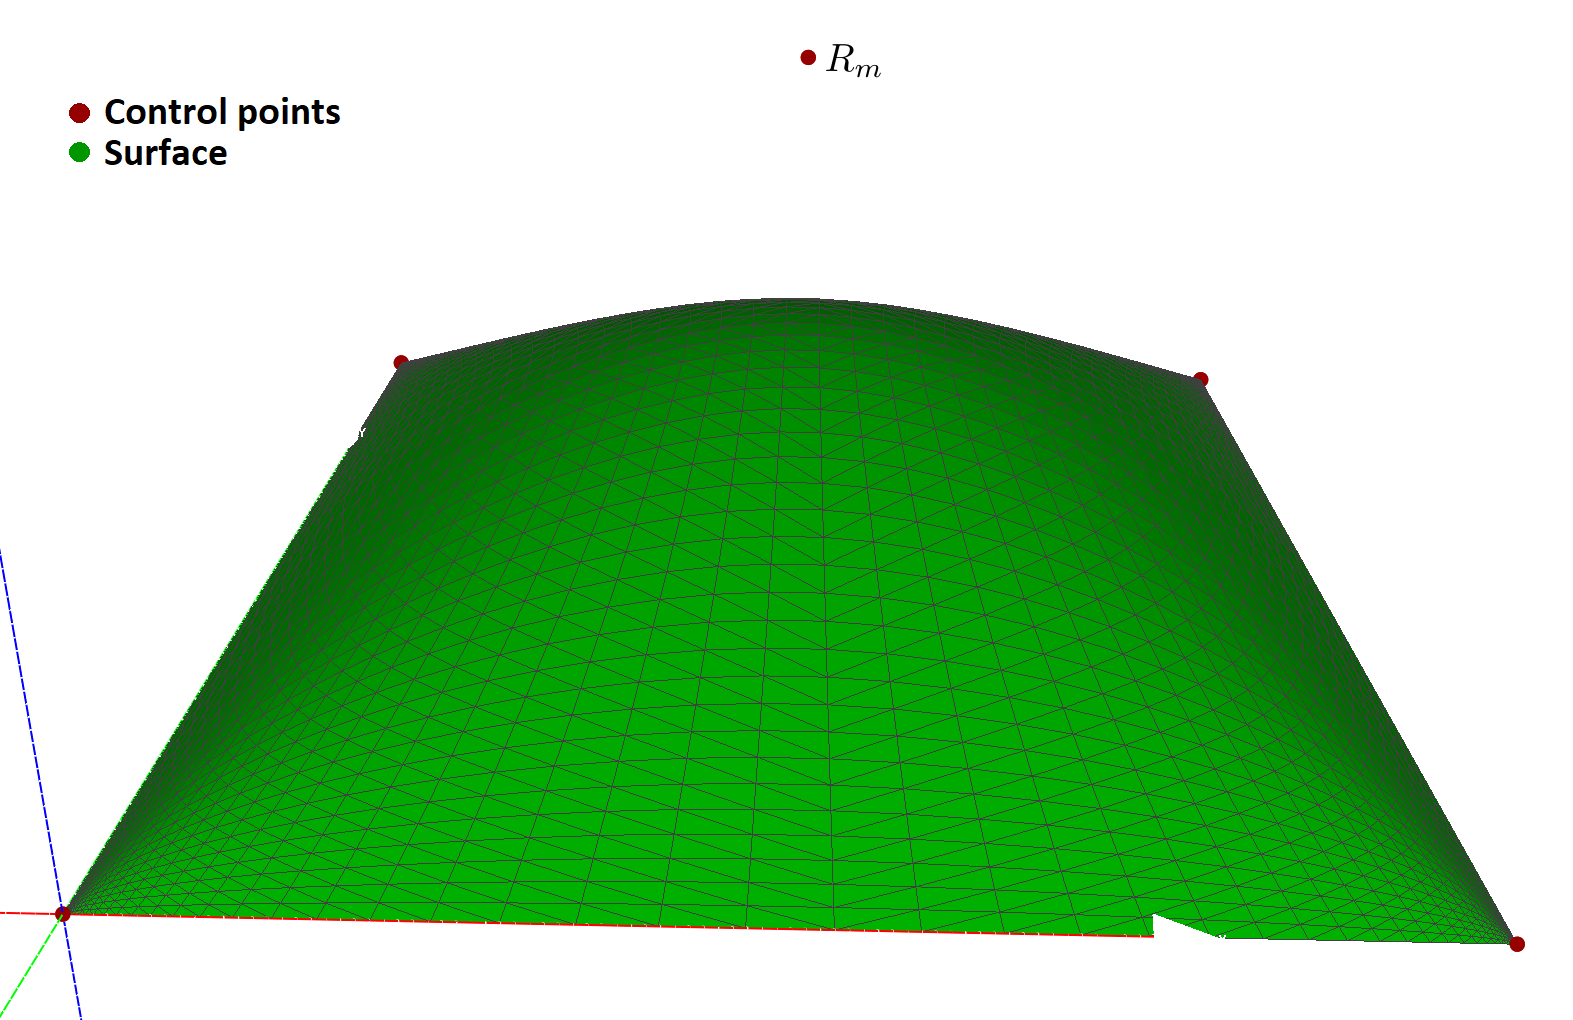
\includegraphics[width=\textwidth]{tsplineex1}
\caption{$\emph{\textbf{t}}_1$ = $\emph{\textbf{t}}_2$ = (0, 0, 0.5, 1, 1)}
\label{tsplineex2}
\end{subfigure}
\begin{subfigure}[b]{0.48\textwidth}
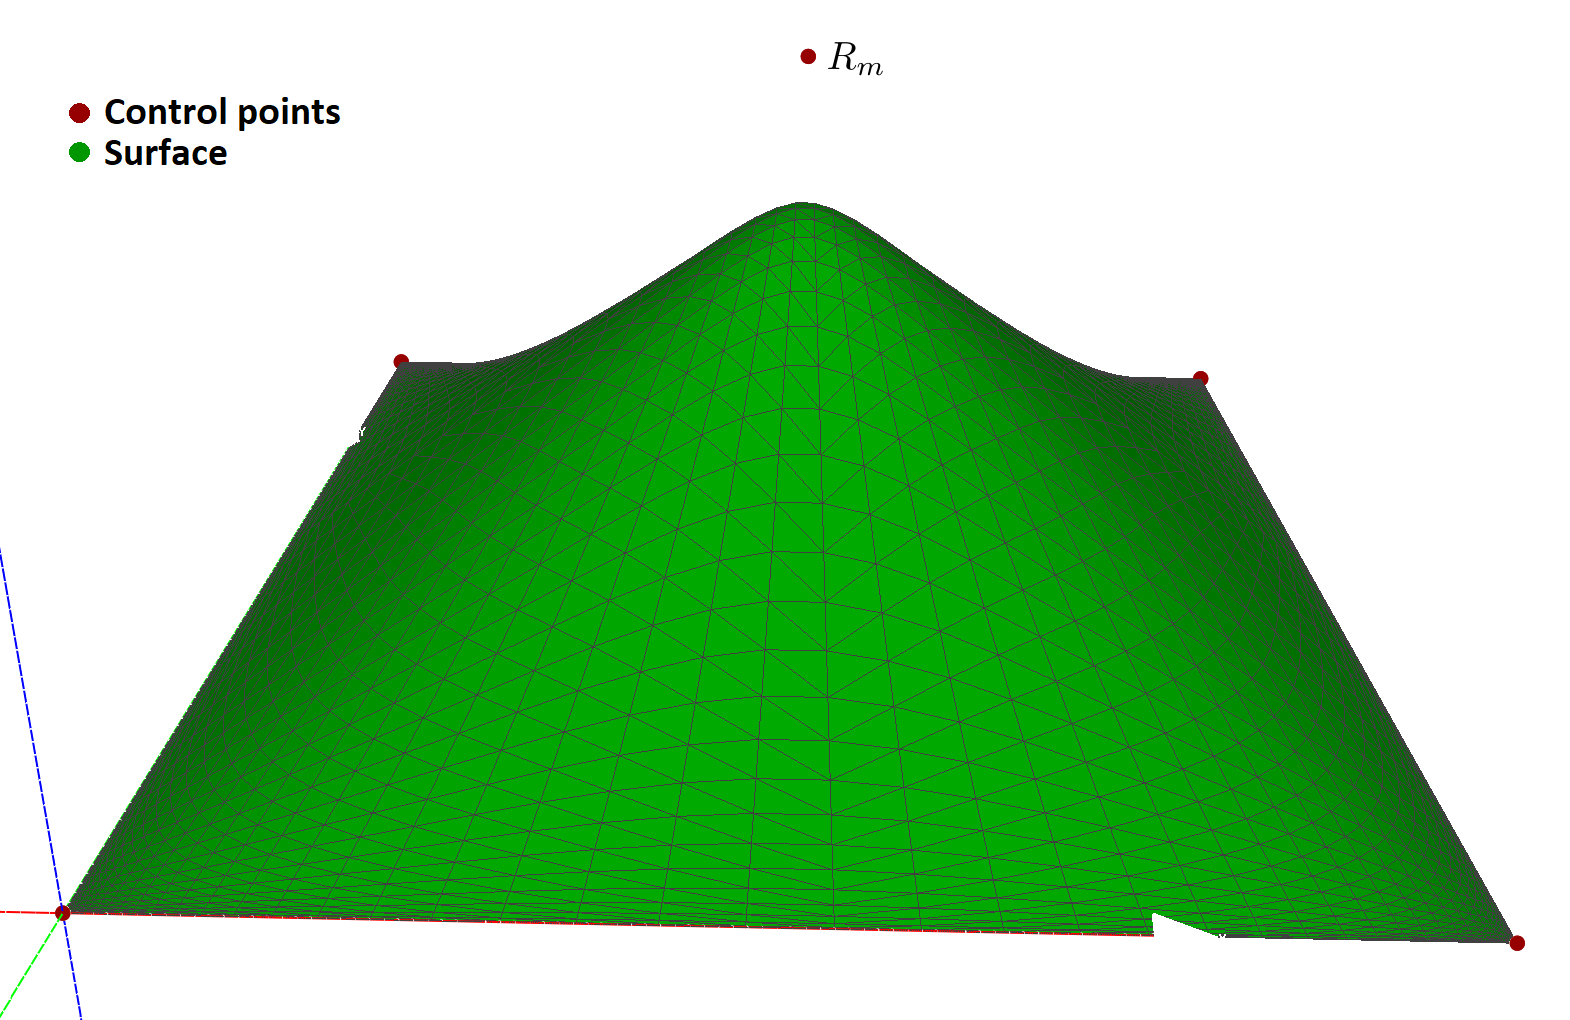
\includegraphics[width=\textwidth]{tsplineex2}
\caption{$\emph{\textbf{t}}_1$ = $\emph{\textbf{t}}_2$ = (0, 0.4, 0.5, 0.6, 1)}
\label{tsplineex2}
\end{subfigure}
\caption{Surfaces with the same T-spline control points, but with different knot vectors of $R_m$.}
\label{tsplineexs}
\end{figure}

For this kind of change in a B-spline surface, the introduction of more control points are inevitable, but in case of T-spline surface, altering the knot vectors is sufficient. This allows the so-called \emph{local refinement} as opposed to \emph{global refinement} which is the only possible solution with the B-spline approach (Sederberg et al., 2004). This will be illustrated through examples in Section \ref{sec:exp} in more detail.

\subsubsection{T-mesh}

\vspace{6pt}

T-mesh is the rectangular grid of parametric space where the knots exist for a specific T-spline surface (Li $\&$ Scott, 2014). It is characterised by the so-called \emph{T-junction} which is a T-shaped edge-edge intersection (Sederberg et al., 2003). This is why a T-spline surface is locally refineable.

\begin{figure}[H]
\centering
\begin{subfigure}[b]{0.48\textwidth}
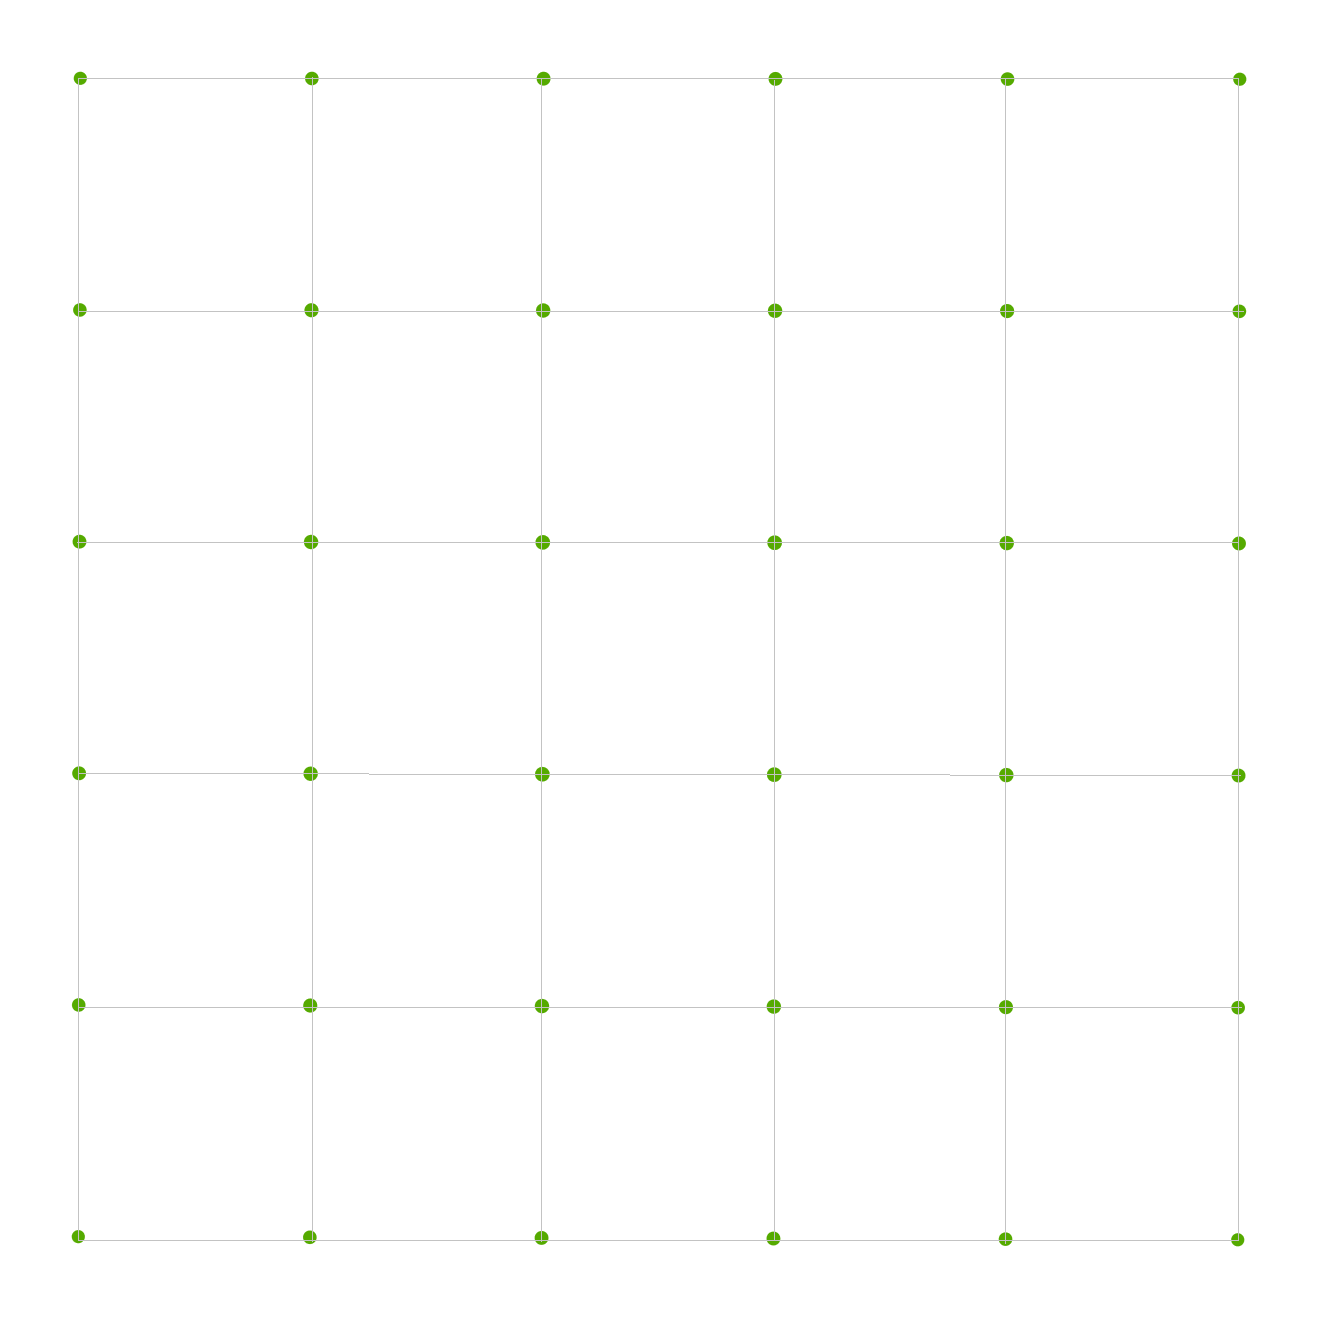
\includegraphics[width=\textwidth]{bsplinegrid}
\caption{B-spline knot grid is always a regular mesh without T-junctions or holes.}
\label{bsplinegrid}
\end{subfigure}
\begin{subfigure}[b]{0.48\textwidth}
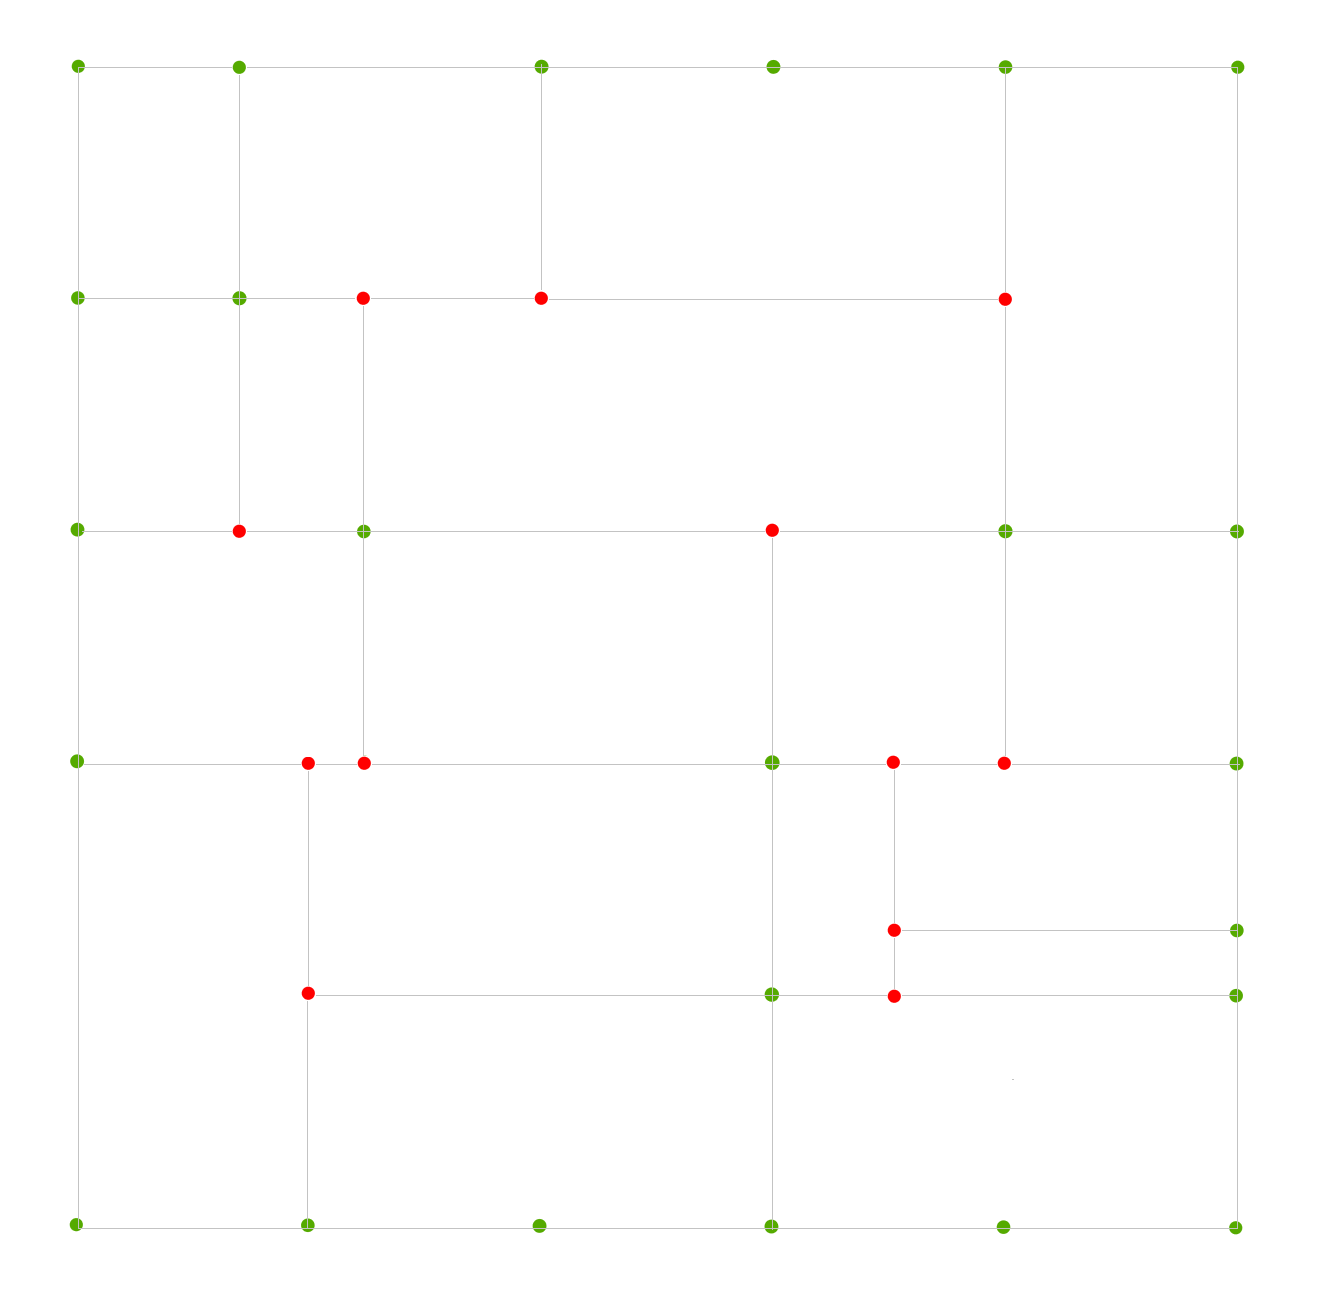
\includegraphics[width=\textwidth]{tsplinegrid}
\caption{T-spline knot grid (\emph{T-mesh}) is a generally nonregular mesh with T-junctions in it.}
\label{tsplinegrid}
\end{subfigure}
\caption{B-spline and T-spline knot meshes of parametric space. The dots represent the knots. Red dots are in a T-junction.}
\label{knotgrids}
\end{figure}

Each control point in a T-spline surface has a central knot in the T-mesh. Their other four knots are not necessarily visible, though. From first knot to last, the full \emph{domain} of a control point can be drawn with a rectangle. This is what is shown in Figure \ref{tmeshdomains}.

\begin{figure}[H]
\centering
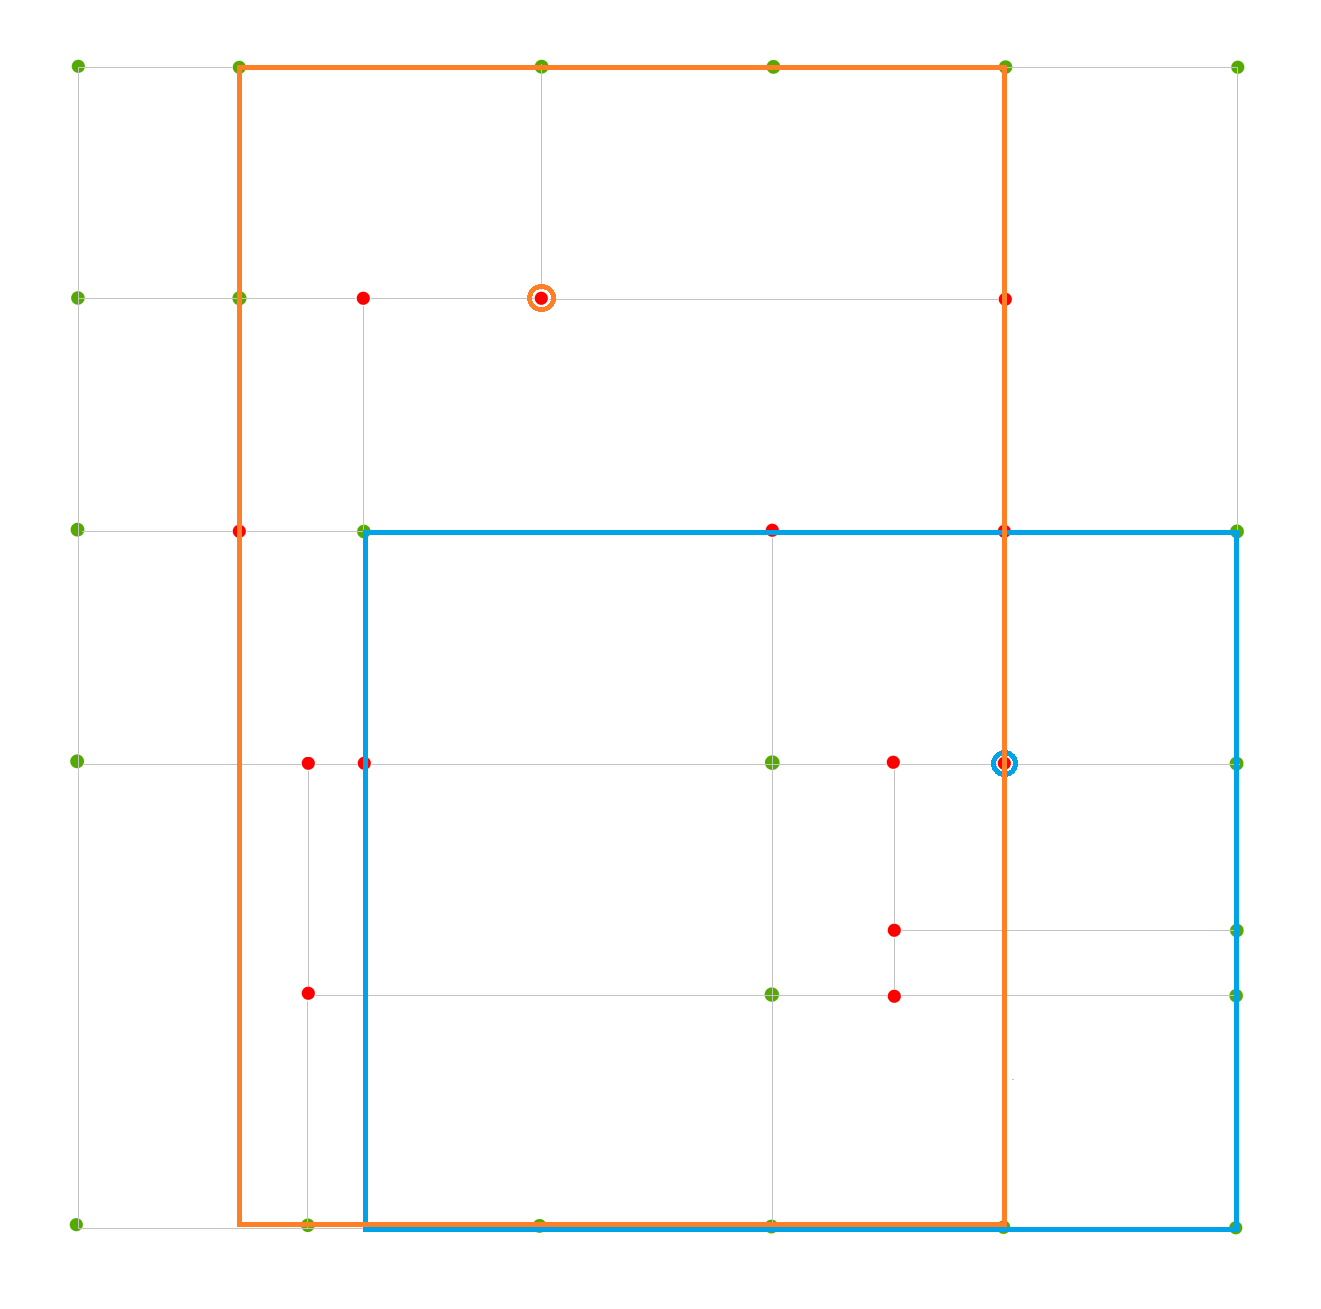
\includegraphics[width=0.48\textwidth]{tsplinegridoverlaps}
\caption{Domains of two (circled) control points. Overlaps indicate common surface area defined by both control points.}
\label{tmeshdomains}
\end{figure}

There are certain rules, how a T-mesh is formed, but this will be omitted here. This essay focuses on knots solely, and how they shape the surface. T-mesh technicalities are explained in great detail in Sederberg et al. (2003) (2004).

\vspace{12pt}

\begin{large}
\section{Code implementation}
\end{large}

\vspace{12pt}

The emphasis of this research is not on writing a perfect, sustainable code, however, implementation is inevitable to experiment. The code is written in Go, and is available on \url{https://github.com/ElleScotZ/project-cs}. This choice was mainly based on my prior knowledge and experience in Go. Also, it is an easily understandable, flexible language. Its syntax is hopefully easy enough for everybody who knows some kind of object oriented programming language.

\begin{figure}[H]
\centering
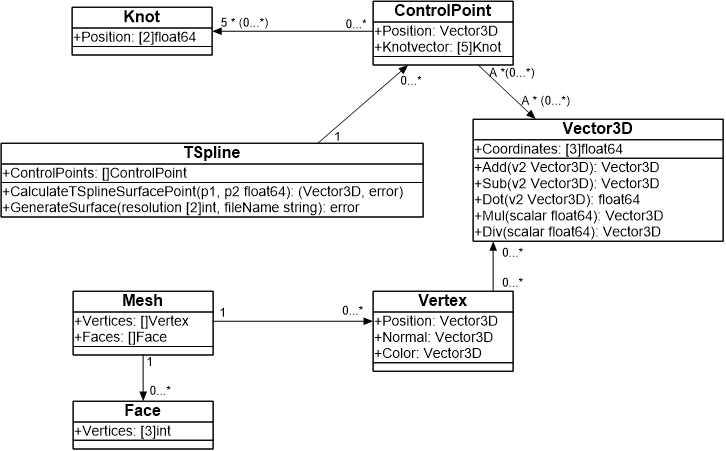
\includegraphics[width=\textwidth]{CD}
\caption{Class diagram of basic code structure. $A$ denotes any non-negative integer.}
\label{classdiagram}
\end{figure}

\begin{table}[H]
\begin{center}
\begin{tabular}{| c | C{4cm} || c | C{4cm}|}
\hline
\textbf{Class name} & \textbf{Class description} & \textbf{Member variable name} & \textbf{Member variable description} \\ \hline \hline
\texttt{Vector3D} & 3D spatial or other type of vector & \texttt{Coordinates} & \emph{x, y, z} or other meaningful coordinates \\ \hline
\multirow{2}{*}{\texttt{ControlPoint}} & \multirow{2}{*}{A control point in 3D} & \texttt{Position} & Coordinates of control point \\ \cline{3-4}
& & \texttt{Knotvector} & Associated 5-knot long 2D knot vector \\ \hline
\texttt{Knot} & A knot in the surface & \texttt{Position} & 2D parametric position \\ \hline
\texttt{TSpline} & T-spline surface & \texttt{ControlPoints} & Control points that define the T-spline surface \\ \hline
\multirow{2}{*}{\texttt{Mesh}} & \multirow{2}{*}{Triangle mesh} & \texttt{Vertices} & Vertices that define surface of mesh \\ \cline{3-4}
& & \texttt{Faces} & Triangle (3-vertex sized) faces of mesh \\ \hline
\multirow{3}{*}{\texttt{Vertex}} & \multirow{3}{*}{Vertex of a mesh} & \texttt{Position} & Coordinates of a vertex \\ \cline{3-4}
& & \texttt{Normal} & Normal vector of vertex \\ \cline{3-4}
& & \texttt{Color} & RGB colour of vertex \\ \hline
\texttt{Face} & 3-vertex sized triangle face & \texttt{Vertices} & Order number of vertices in \texttt{Mesh} \\
\hline
\end{tabular}
\end{center}
\caption{Short description of each class and their member variables.}
\label{codetable}
\end{table}

\subsection{Code execution}

\vspace{6pt}
Assuming you have already downloaded Visual Studio Code and Go, and you know how to use basic Git, follow the instructions below on how to run the code.

\begin{enumerate}
\item Clone the GitHub repository \url{https://github.com/ElleScotZ/project-cs}.

\item Open a terminal and in the \texttt{root} repository, type in \texttt{go run main.go}.

\item Open the created \texttt{out} folder with the generated PLY files in it.

\item Open PLY with Print 3D (on Windows), if you do not have anything else\footnote{I personally use Meshlab.}.
\end{enumerate}

\vspace{12pt}

\begin{large}
\section{T-spline surface variations}
\label{sec:exp}
\end{large}

\vspace{12pt}

It is time to experiment with different knot vectors on the same set of 9 control points to understand their effects on the T-spline surface. The coordinate of these control points are available in \texttt{main.go} in \texttt{line 1474-1482} and also in Table \ref{cps}. The order of the control points indicates only their order in the array in the code.

\begin{table}[H]
\centering
\begin{tabular}{| c | c |}
\hline
$R_1$ & (-1.00, 0.00, 5.00) \\ \hline
$R_2$ & (1.00, 0.00, 5.00) \\ \hline
$R_3$ & (2.50, 3.50, 0.00) \\ \hline
$R_4$ & (1.00, 5.00, 5.00) \\ \hline
$R_5$ & (-2.50, 3.50, 0.00) \\ \hline
$R_6$ & (-2.50, 1.50, 0.00) \\ \hline
$R_7$ & (1.75, 0.75, 2.50) \\ \hline
$R_8$ & (1.75, 4.25, 2.50) \\ \hline
$R_9$ & (0.00, 2.50, 4.00) \\
\hline
\end{tabular}
\caption{The 9 control points that are used to create T-spline surfaces during this essay.}
\label{cps}
\end{table}

Throughout the examples, $\textbf{T}$ will denote a generic two-dimensional knot vector that does not belong to any specific control point. The $\textbf{t}_i$, however, will mean a specific knot vector that belongs to $R_i$. For further reference, see Table \ref{denotions}.

\begin{table}[H]
\centering
\begin{tabular}{| c | c | c | c |}
\hline
\textbf{Symbol} & \textbf{Description} & \multicolumn{2}{c |}{\textbf{Example}} \\ \hline
$\textbf{T}$ & not control point specific 2D knot vector & \multicolumn{2}{c |}{([0,0], [0,1], [1,1], [2,1], [2,2])} \\ \hline
$\textbf{T}_k$ & $k$th knot in $\textbf{T}$ & $k$ = 2 & [0,1] \\ \hline
$\textbf{T}_{k, 1}$ & first dimensional coordinate of $\textbf{T}_k$ & $k$ = 2 & 0 \\ \hline
$\textbf{T}_{k, 2}$ & second dimensional coordinate of $\textbf{T}_k$  & $k$ = 2 & 1 \\ \hline \hline
$\textbf{t}_i$ & 2D knot vector of $R_i$ & \multicolumn{2}{c |}{([0,0], [0,1], [1,1], [2,1], [2,2])} \\ \hline
$\textbf{t}_{i, k}$ & $k$th knot in $\textbf{t}_i$ & $k$ = 4 & [2,1] \\ \hline
$\textbf{t}_{i, k, 1}$ & first dimensional coordinate of $\textbf{t}_{i, k}$ $\textbf{T}_k$ & $k$ = 4 & 2 \\ \hline
$\textbf{t}_{i, k, 2}$ & second dimensional coordinate of $\textbf{t}_{i,k}$  & $k$ = 4 & 1 \\
\hline
\end{tabular}
\caption{Meaning of different notions.}
\label{denotions}
\end{table}

\subsection{$\textbf{T}_1$ and $\textbf{T}_3$ shift to $\textbf{T}_0$ and $\textbf{T}_4$ along border}

\vspace{6pt}

Let us first demonstrate the shape shifting of a surface of the aforementioned control points from Table \ref{cps} in the following scenario shown in Figure \ref{saddle1p}, and set in details in \texttt{saddle1a()} and \texttt{saddle1b()} in \texttt{main.go}.



\begin{figure}[H]
\centering
\begin{subfigure}[b]{0.48\textwidth}
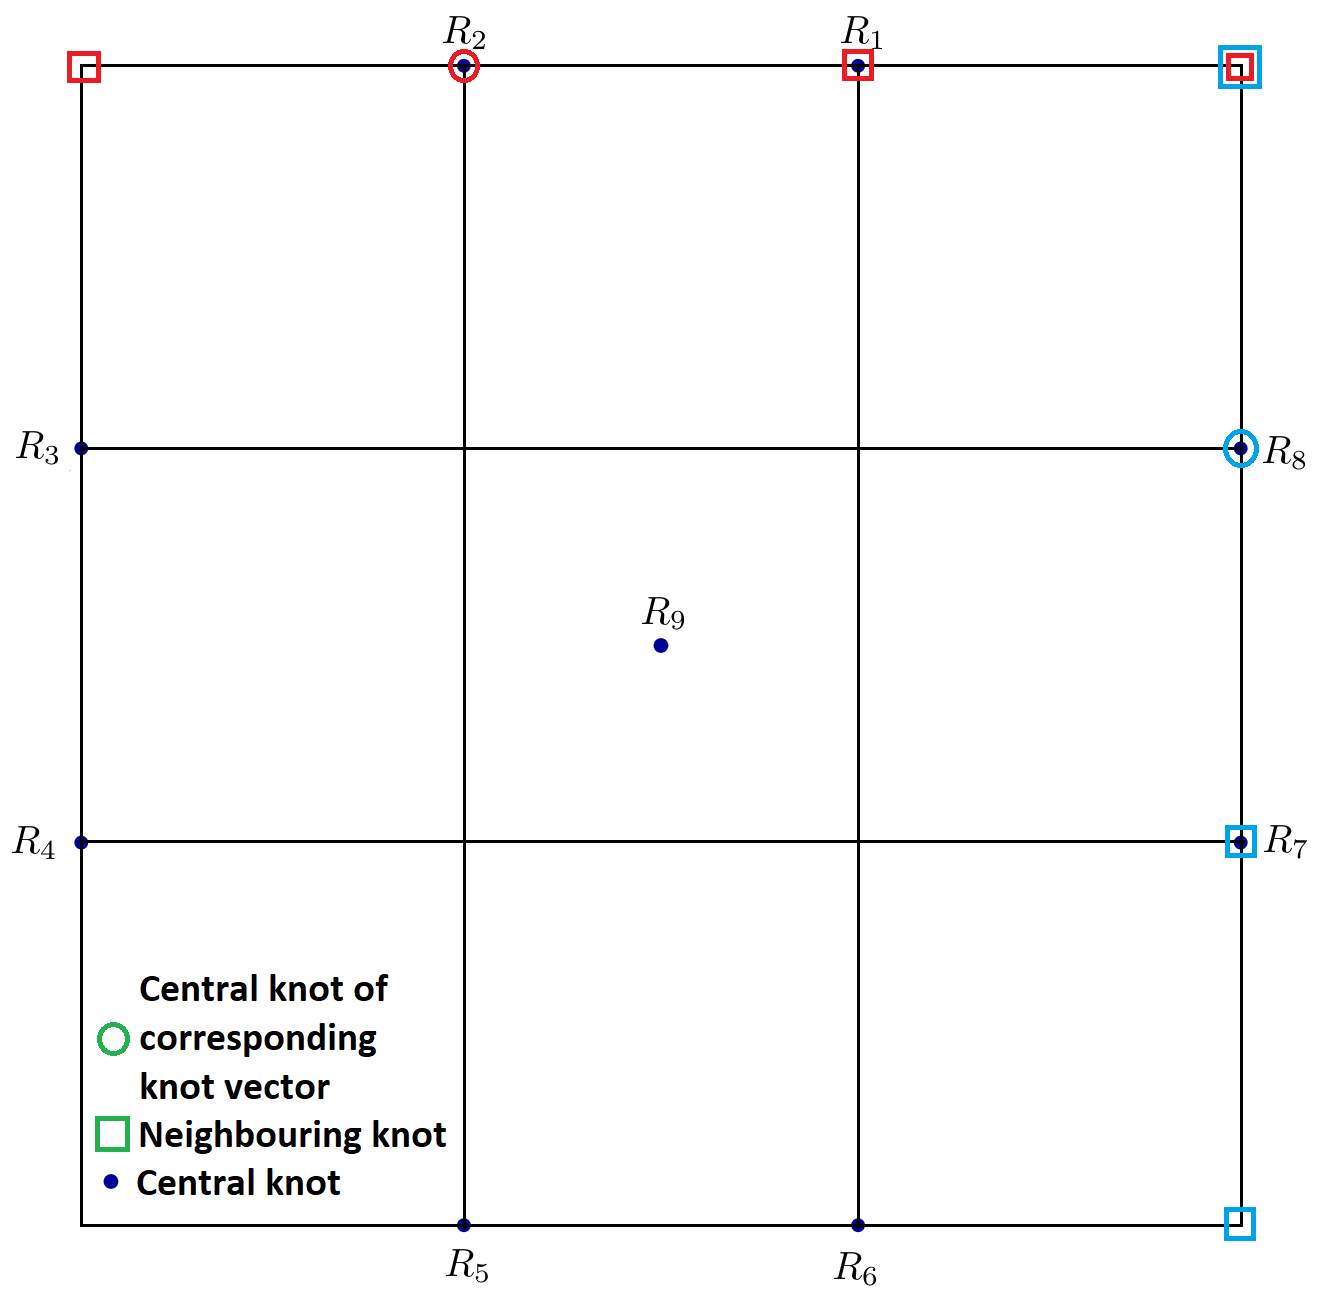
\includegraphics[width=\textwidth]{saddle1aparam}
\caption{Parametric space of \texttt{saddle1a} with two examples (red and blue) of a knot vector distributed across the grid.}
\label{saddle1ap}
\end{subfigure}
\begin{subfigure}[b]{0.48\textwidth}
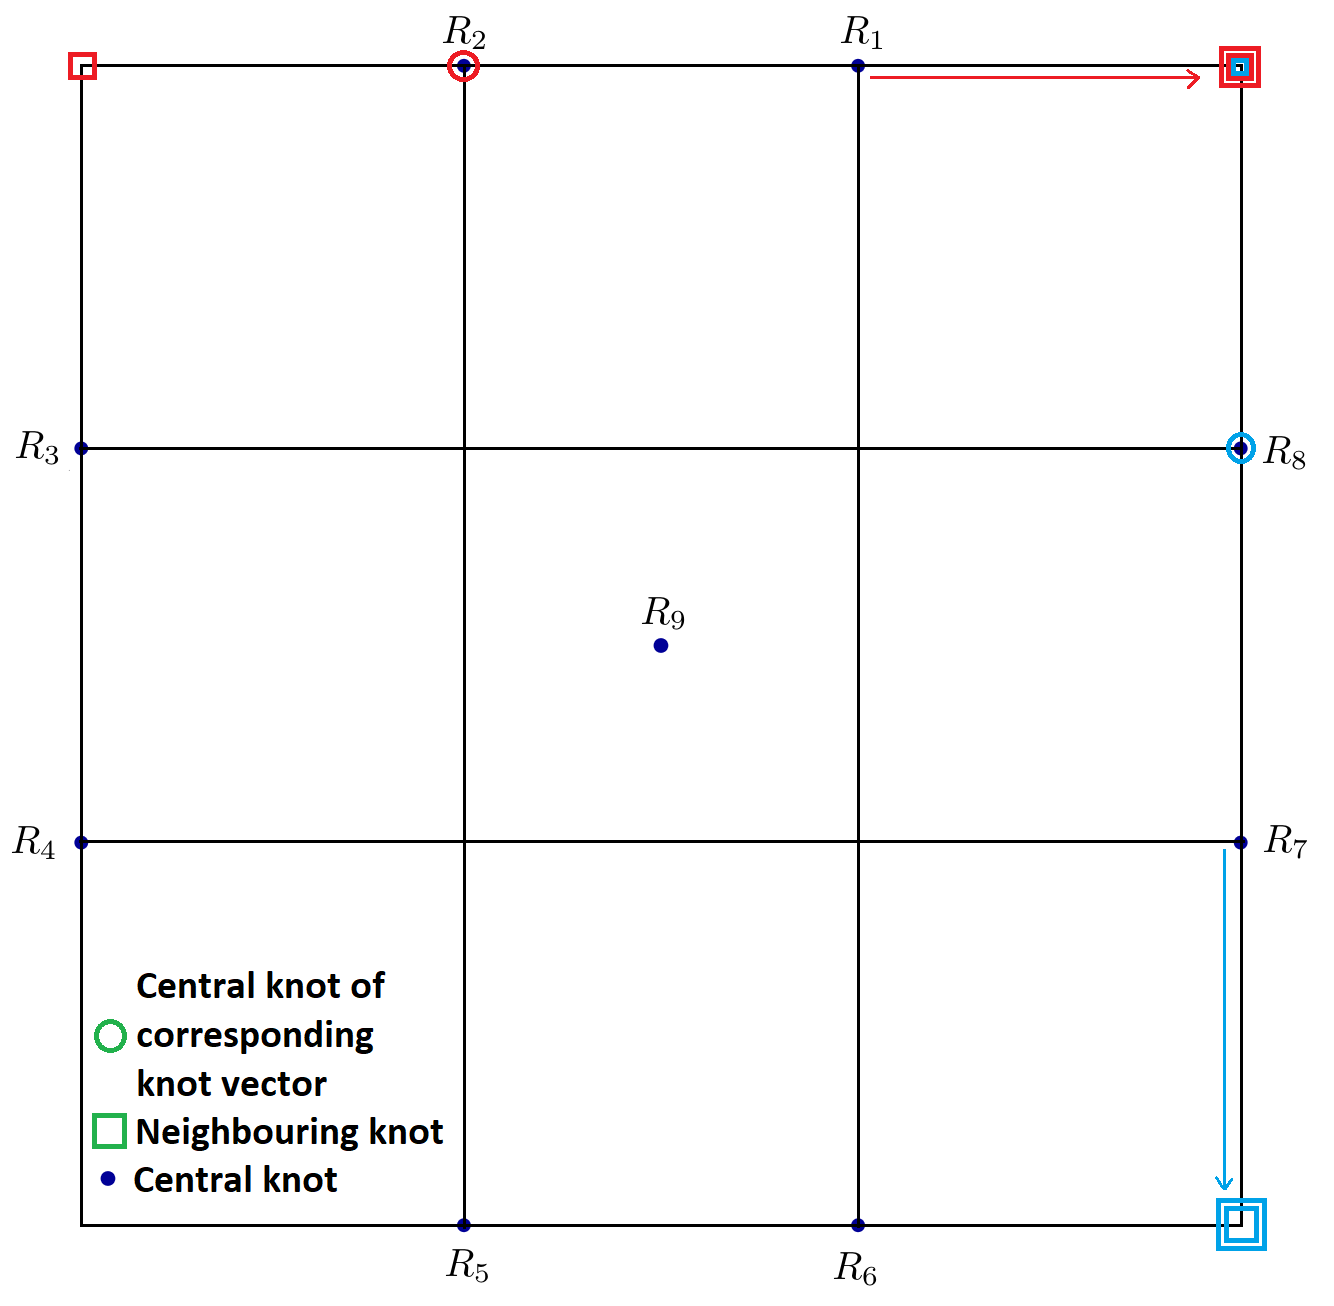
\includegraphics[width=\textwidth]{saddle1bparam}
\caption{Parametric space of \texttt{saddle1b} with the same two examples with an emphasis on change of $T_1$ and $T_3$ knots with arrows.}
\label{saddle1bp}
\end{subfigure}
\caption{Parametric space of each surface. The central knots of control points are represented in a blue point. Circle denotes the central, rectangle does the neighbouring (all, but not central) knots of a knot vector of the corresponding control point.}
\label{saddle1p}
\end{figure}

The knot vector of border control points $R_1$, ..., $R_8$ change from \texttt{saddle1a} to \texttt{saddle1b}. $T_1$ and $T_3$ along the border shift, and merge to $T_0$ and $T_4$, respectively. This will extend the primary AOE of each border control point along the border. Since $T_0$ = $T_1$ and $T_3$ = $T_4$, more $m_i,k(p)$ = 0. Parts that were primarily affected by 2 control points now are affected by 3, so the curve of the border shrinks. Why? The more points attract a specific domain (curve), the shorter the curve tries to be. With that, the curve becomes flatter, so the surface shrinks along the border. This is illustrated in Figure \ref{saddle1}.

\begin{figure}[H]
\centering
\begin{subfigure}[b]{0.48\textwidth}
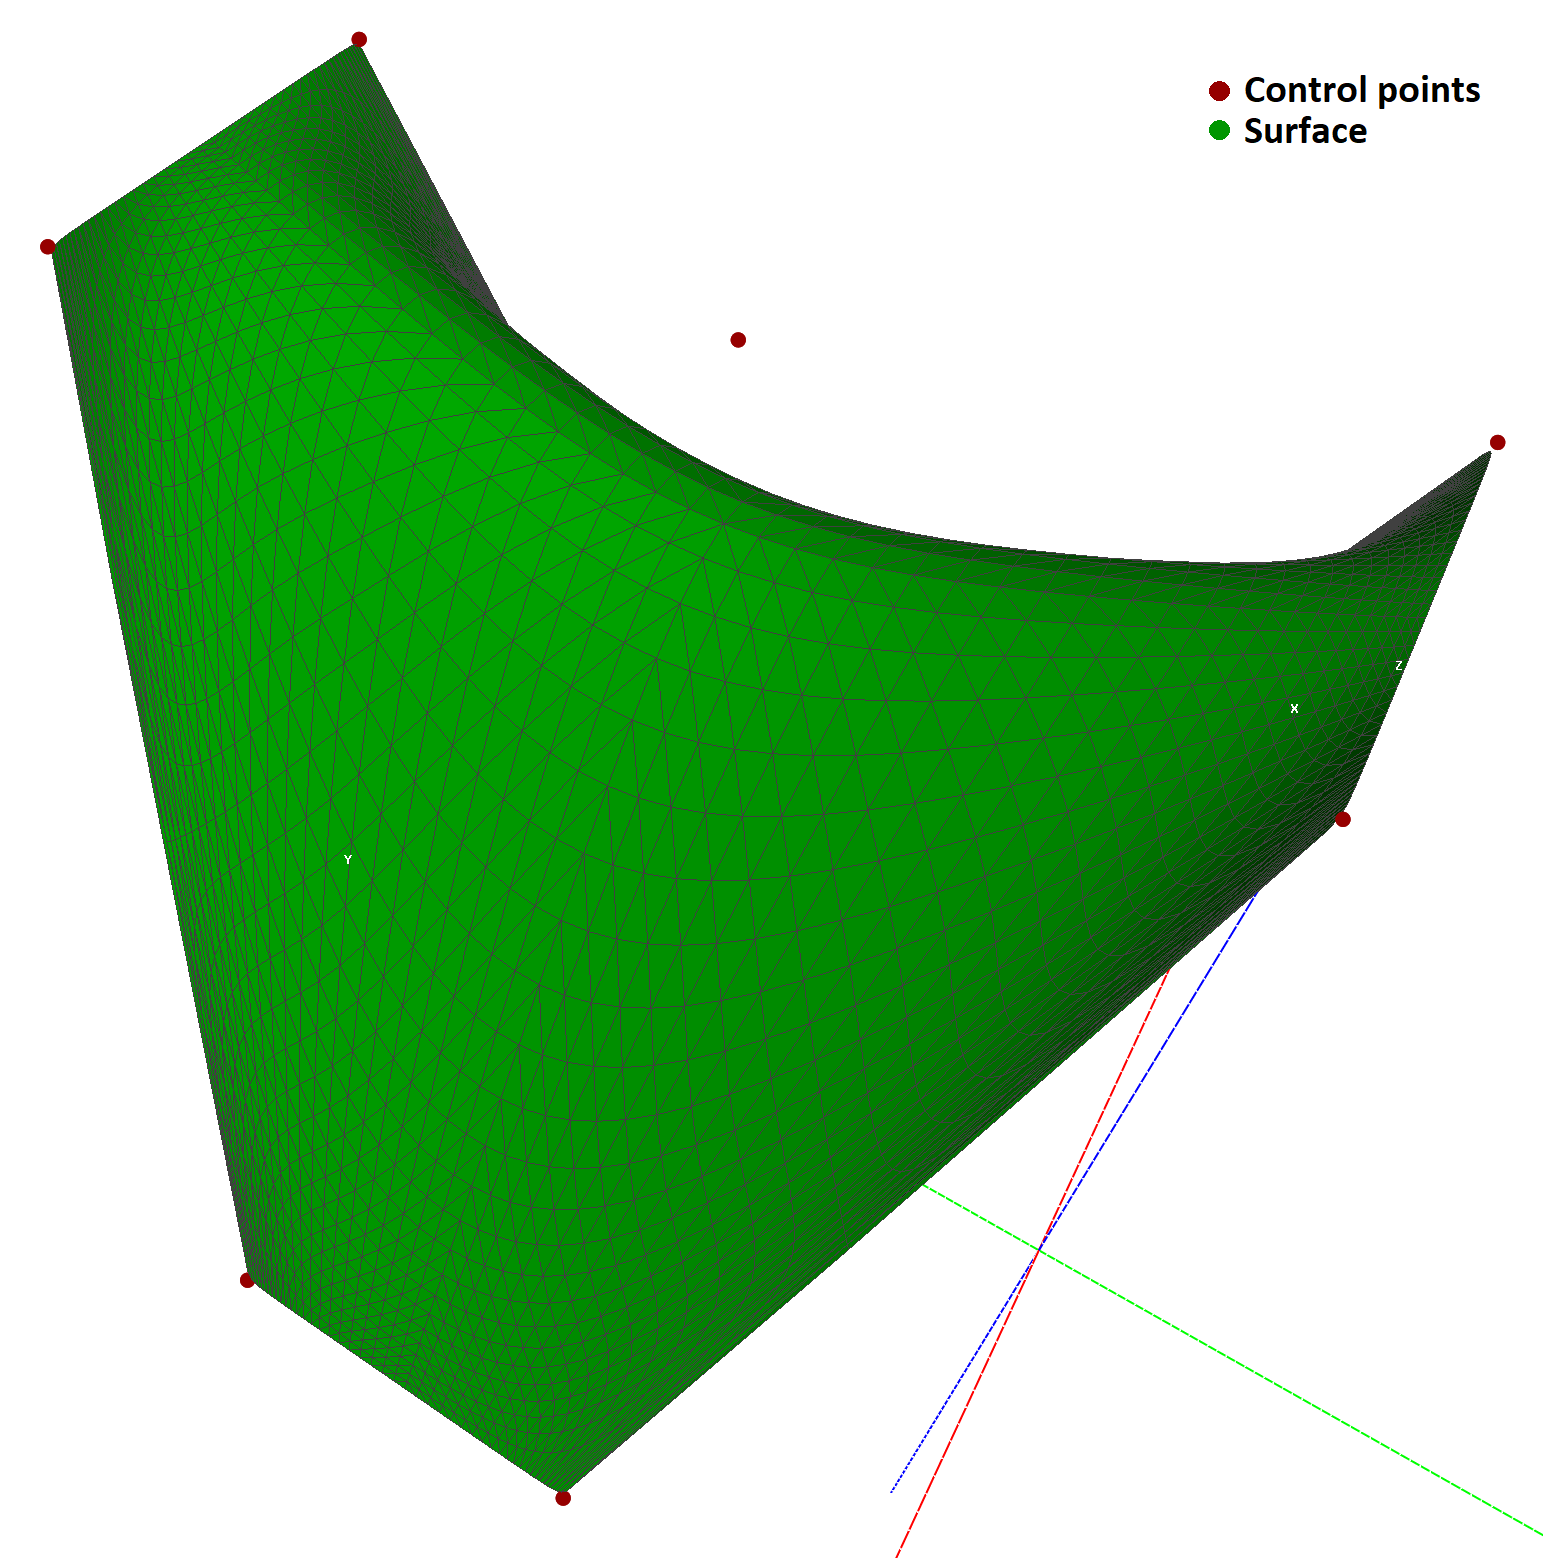
\includegraphics[width=\textwidth]{saddle1a}
\caption{Surface of \texttt{saddle1a}.}
\label{saddle1a}
\end{subfigure}
\begin{subfigure}[b]{0.48\textwidth}
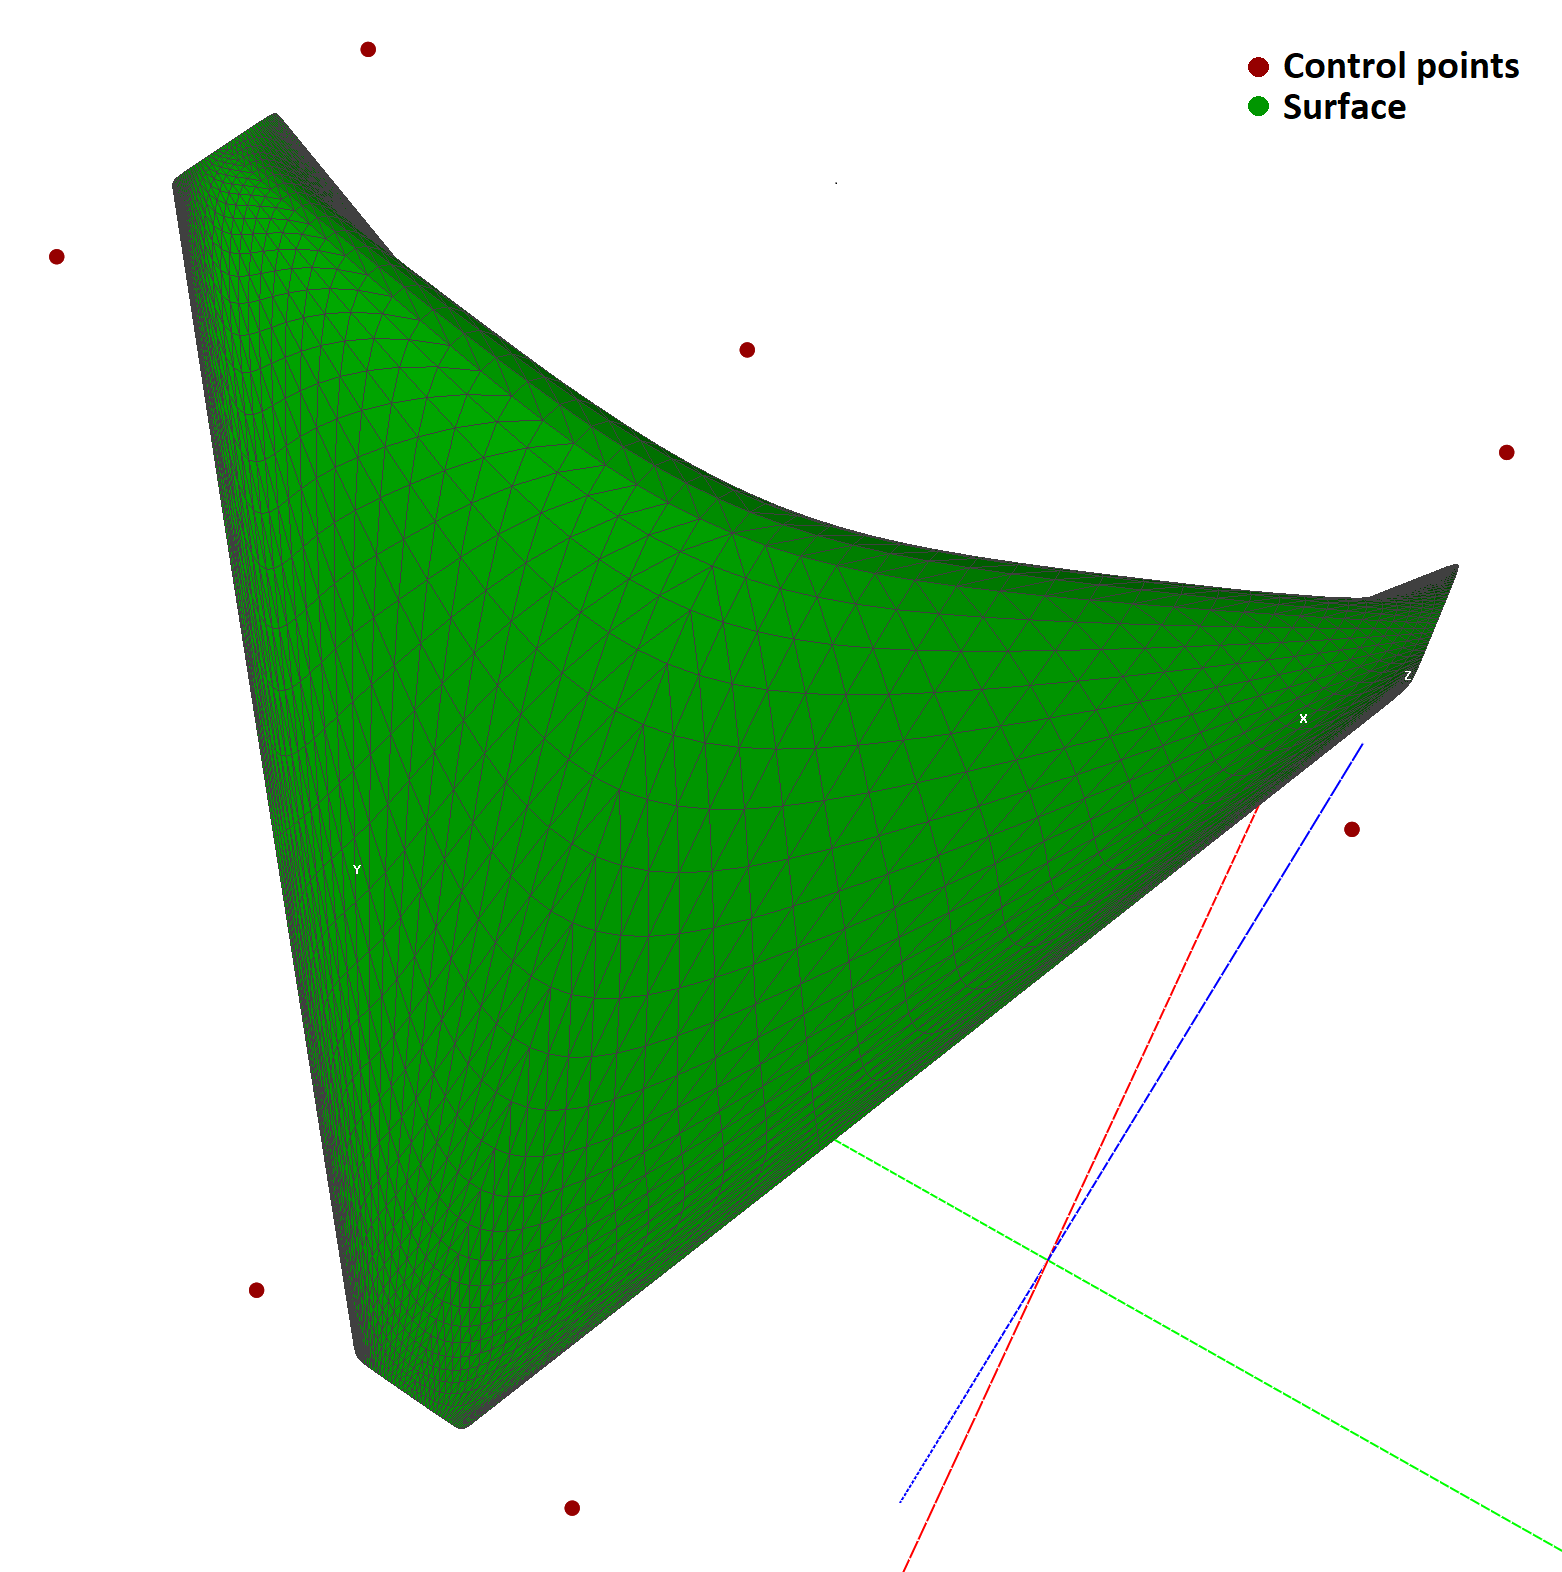
\includegraphics[width=\textwidth]{saddle1b}
\caption{Surface of \texttt{saddle1b}.}
\label{saddle1b}
\end{subfigure}
\caption{T-spline surfaces of \texttt{saddle1}. Surface shrinkage is visible along the border.}
\label{saddle1}
\end{figure}

\subsection{$\textbf{T}_1$ and $\textbf{T}_3$ shift to $\textbf{T}_0$ and $\textbf{T}_4$ inside surface}

\vspace{6pt}

In the second example, the same control points are used, but the knot vector of the middle one $R_9$ is shifted: $t_{9, 1}$ to $t_{9, 0}$, and $t_{9, 3}$ to $t_{9, 4}$.

\begin{figure}[H]
\centering
\begin{subfigure}[b]{0.48\textwidth}
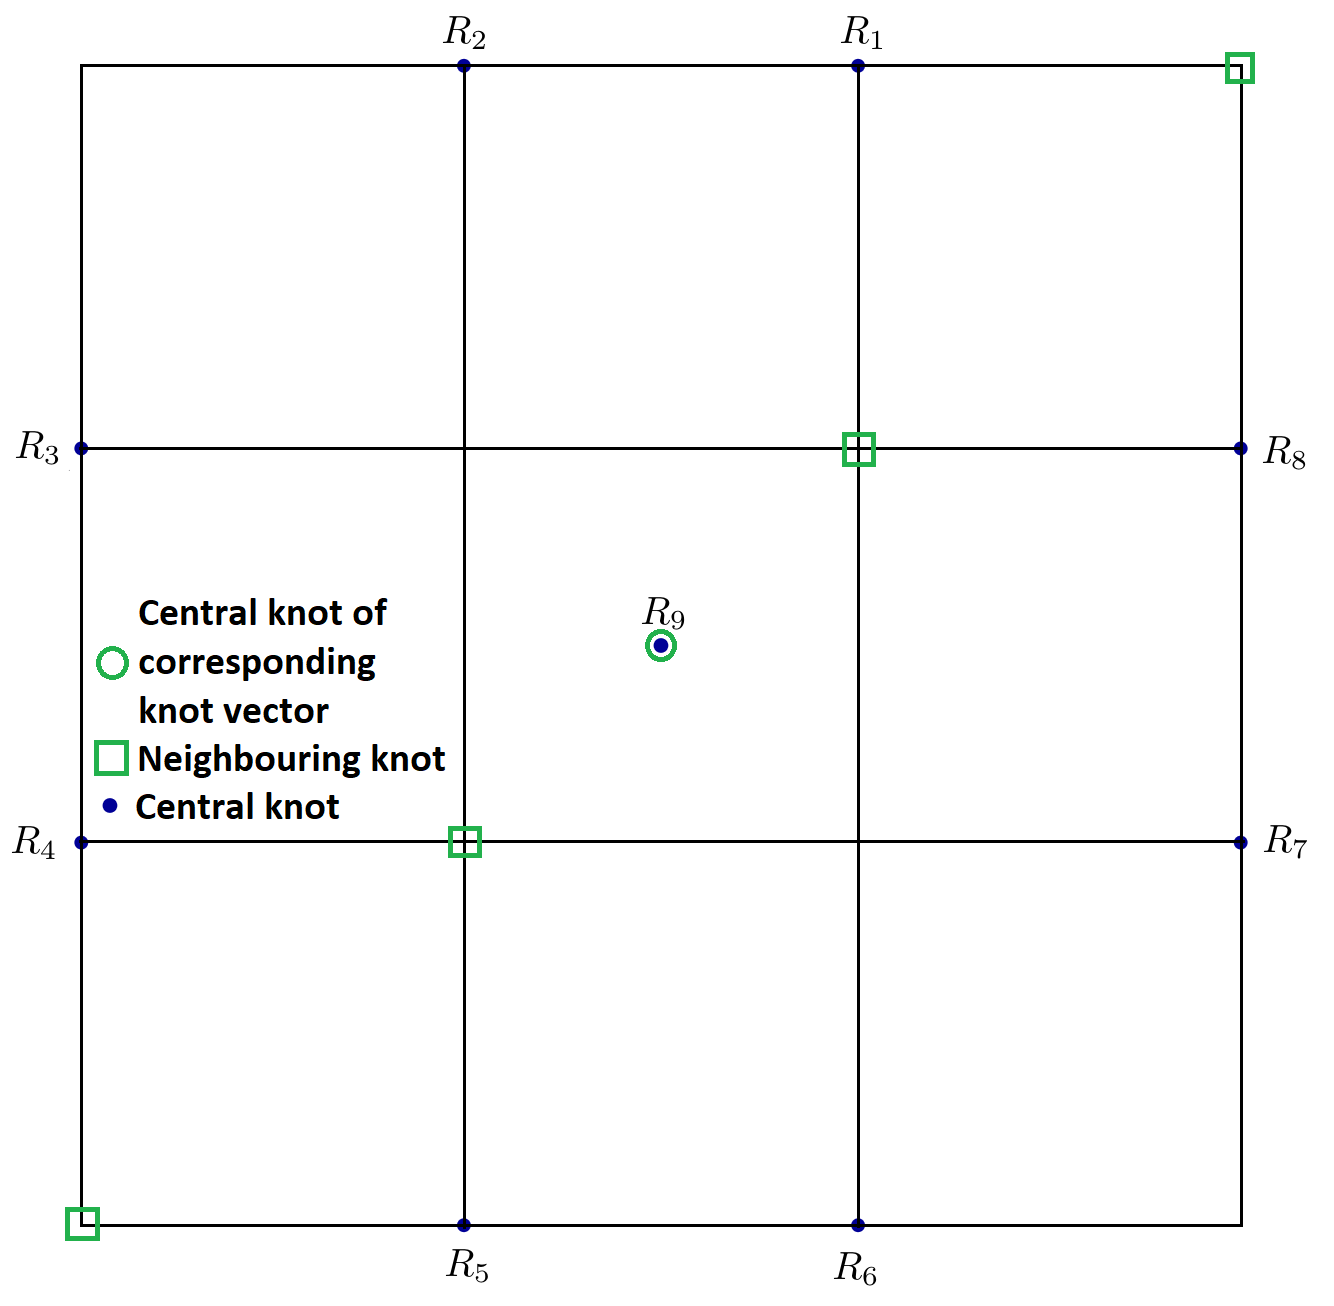
\includegraphics[width=\textwidth]{saddle2aparam}
\caption{\texttt{saddle2a}}
\label{saddle2ap}
\end{subfigure}
\begin{subfigure}[b]{0.48\textwidth}
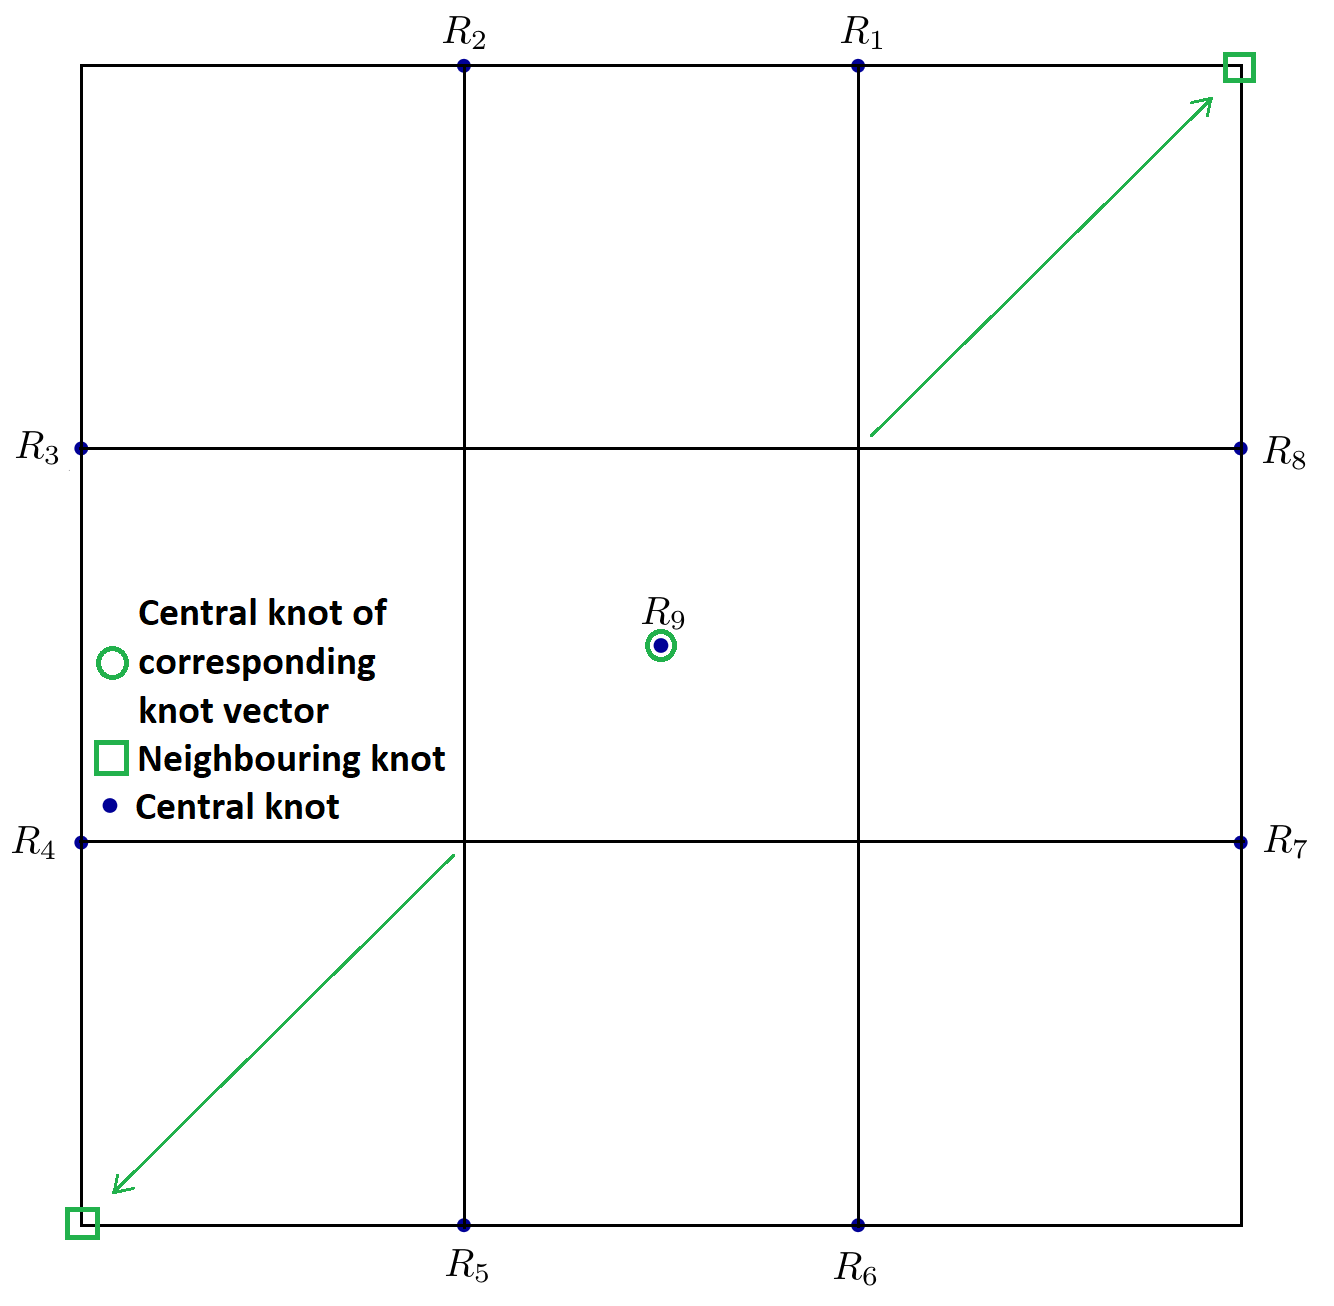
\includegraphics[width=\textwidth]{saddle2bparam}
\caption{\texttt{saddle2b}}
\label{saddle2bp}
\end{subfigure}
\caption{Parametric space of each surface.}
\label{saddle2p}
\end{figure}

The result is expected to be similar to \texttt{saddle1}: the surface will get flatter. The central part of the surface will be less affected by $R_9$, because the primary AOE will have been extended, so more control points will have a say in the shape of the surface.

\begin{figure}[H]
\centering
\begin{subfigure}[b]{0.48\textwidth}
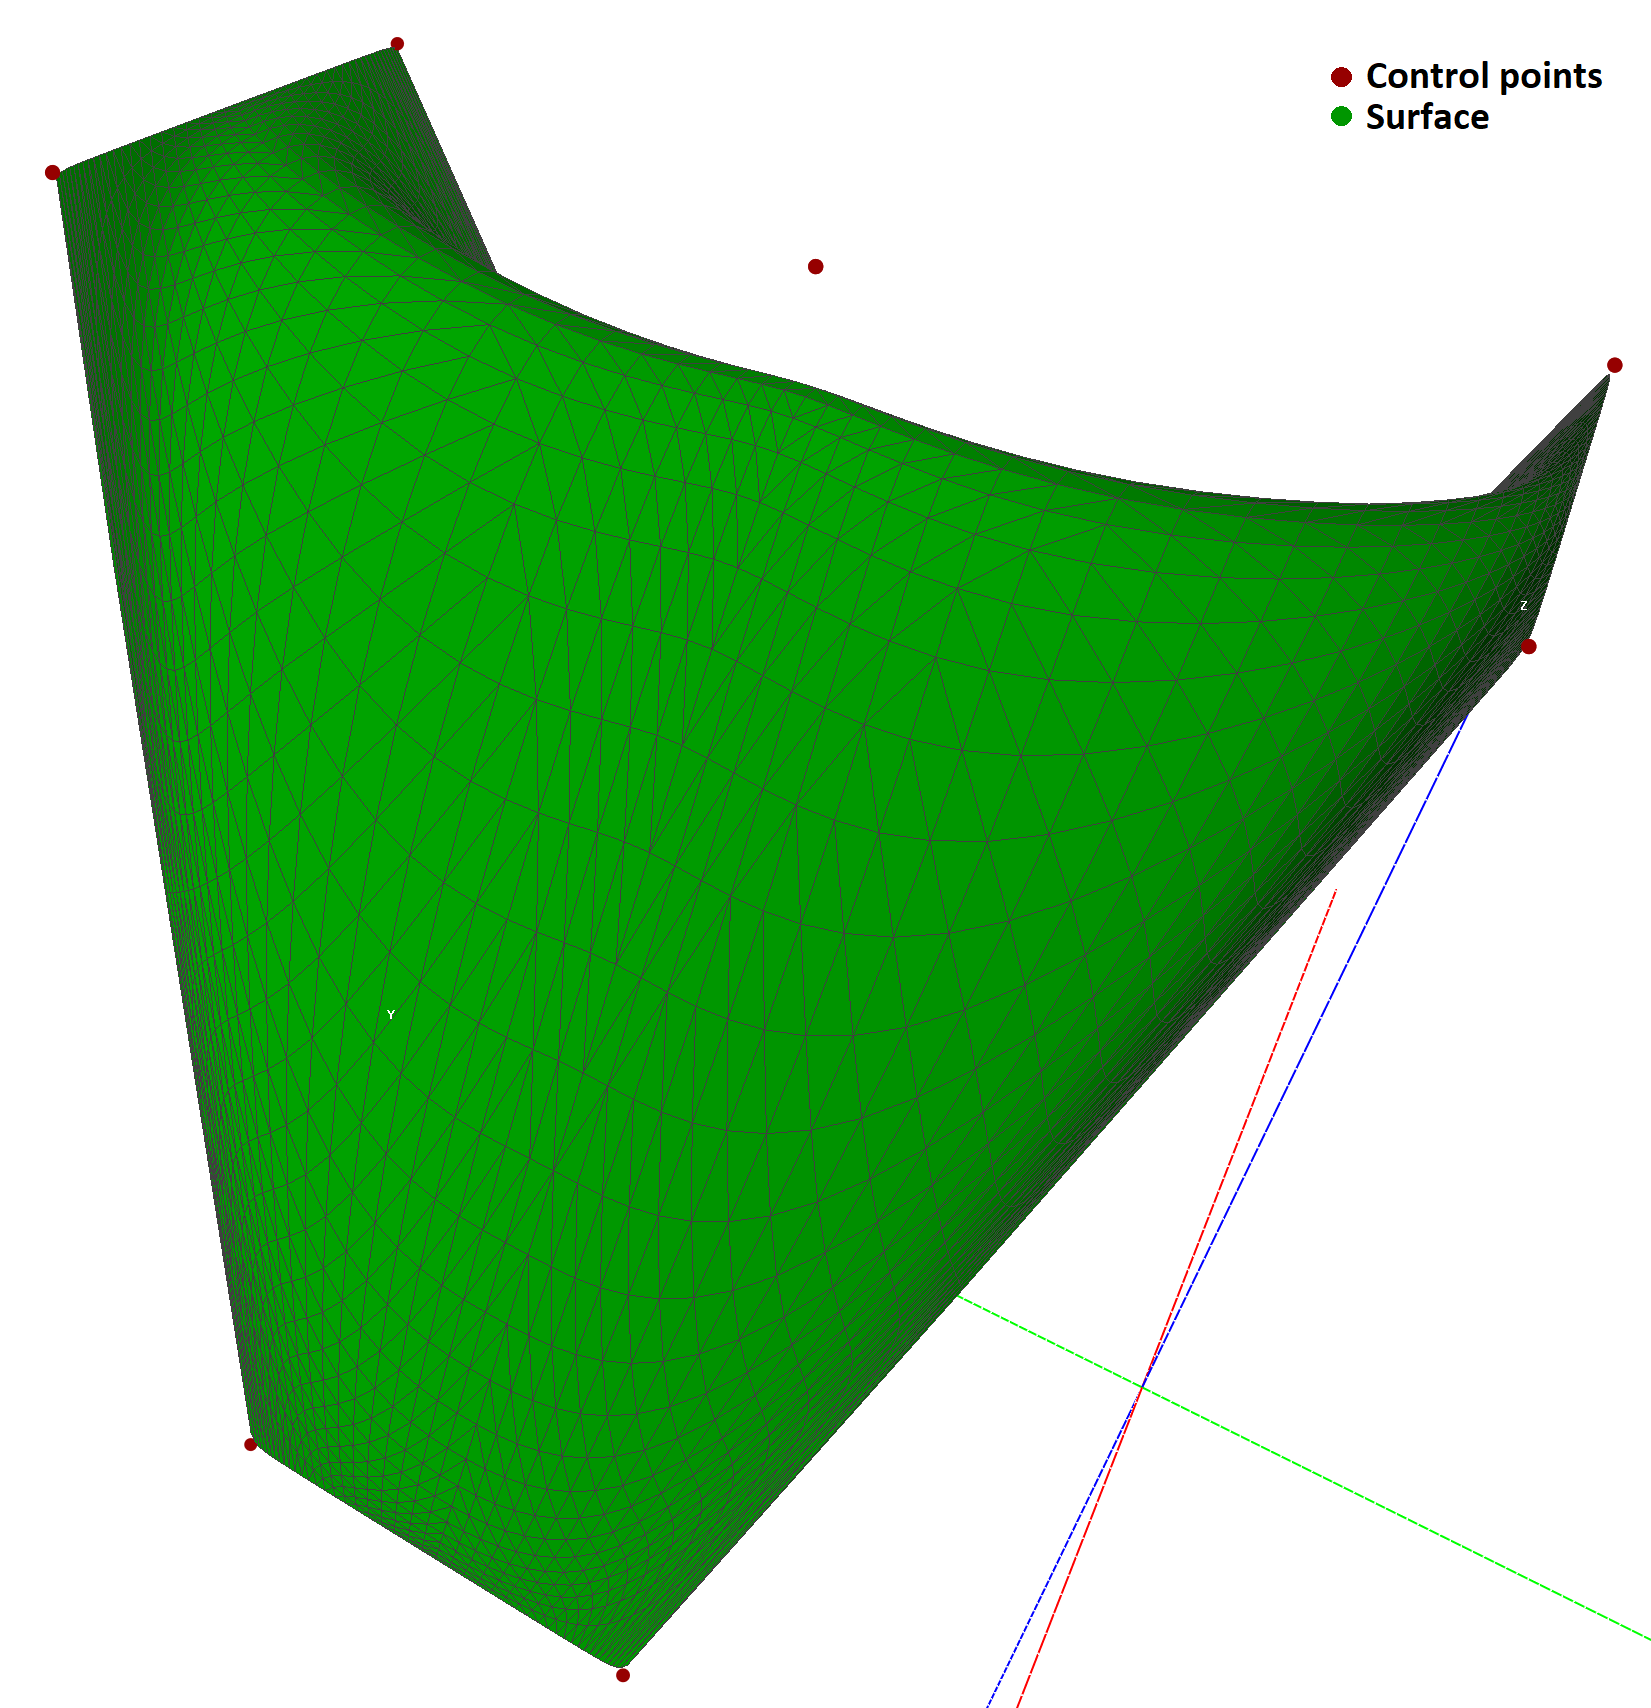
\includegraphics[width=\textwidth]{saddle2a}
\caption{Bump in the middle in \texttt{saddle2a}.}
\label{saddle2a}
\end{subfigure}
\begin{subfigure}[b]{0.48\textwidth}
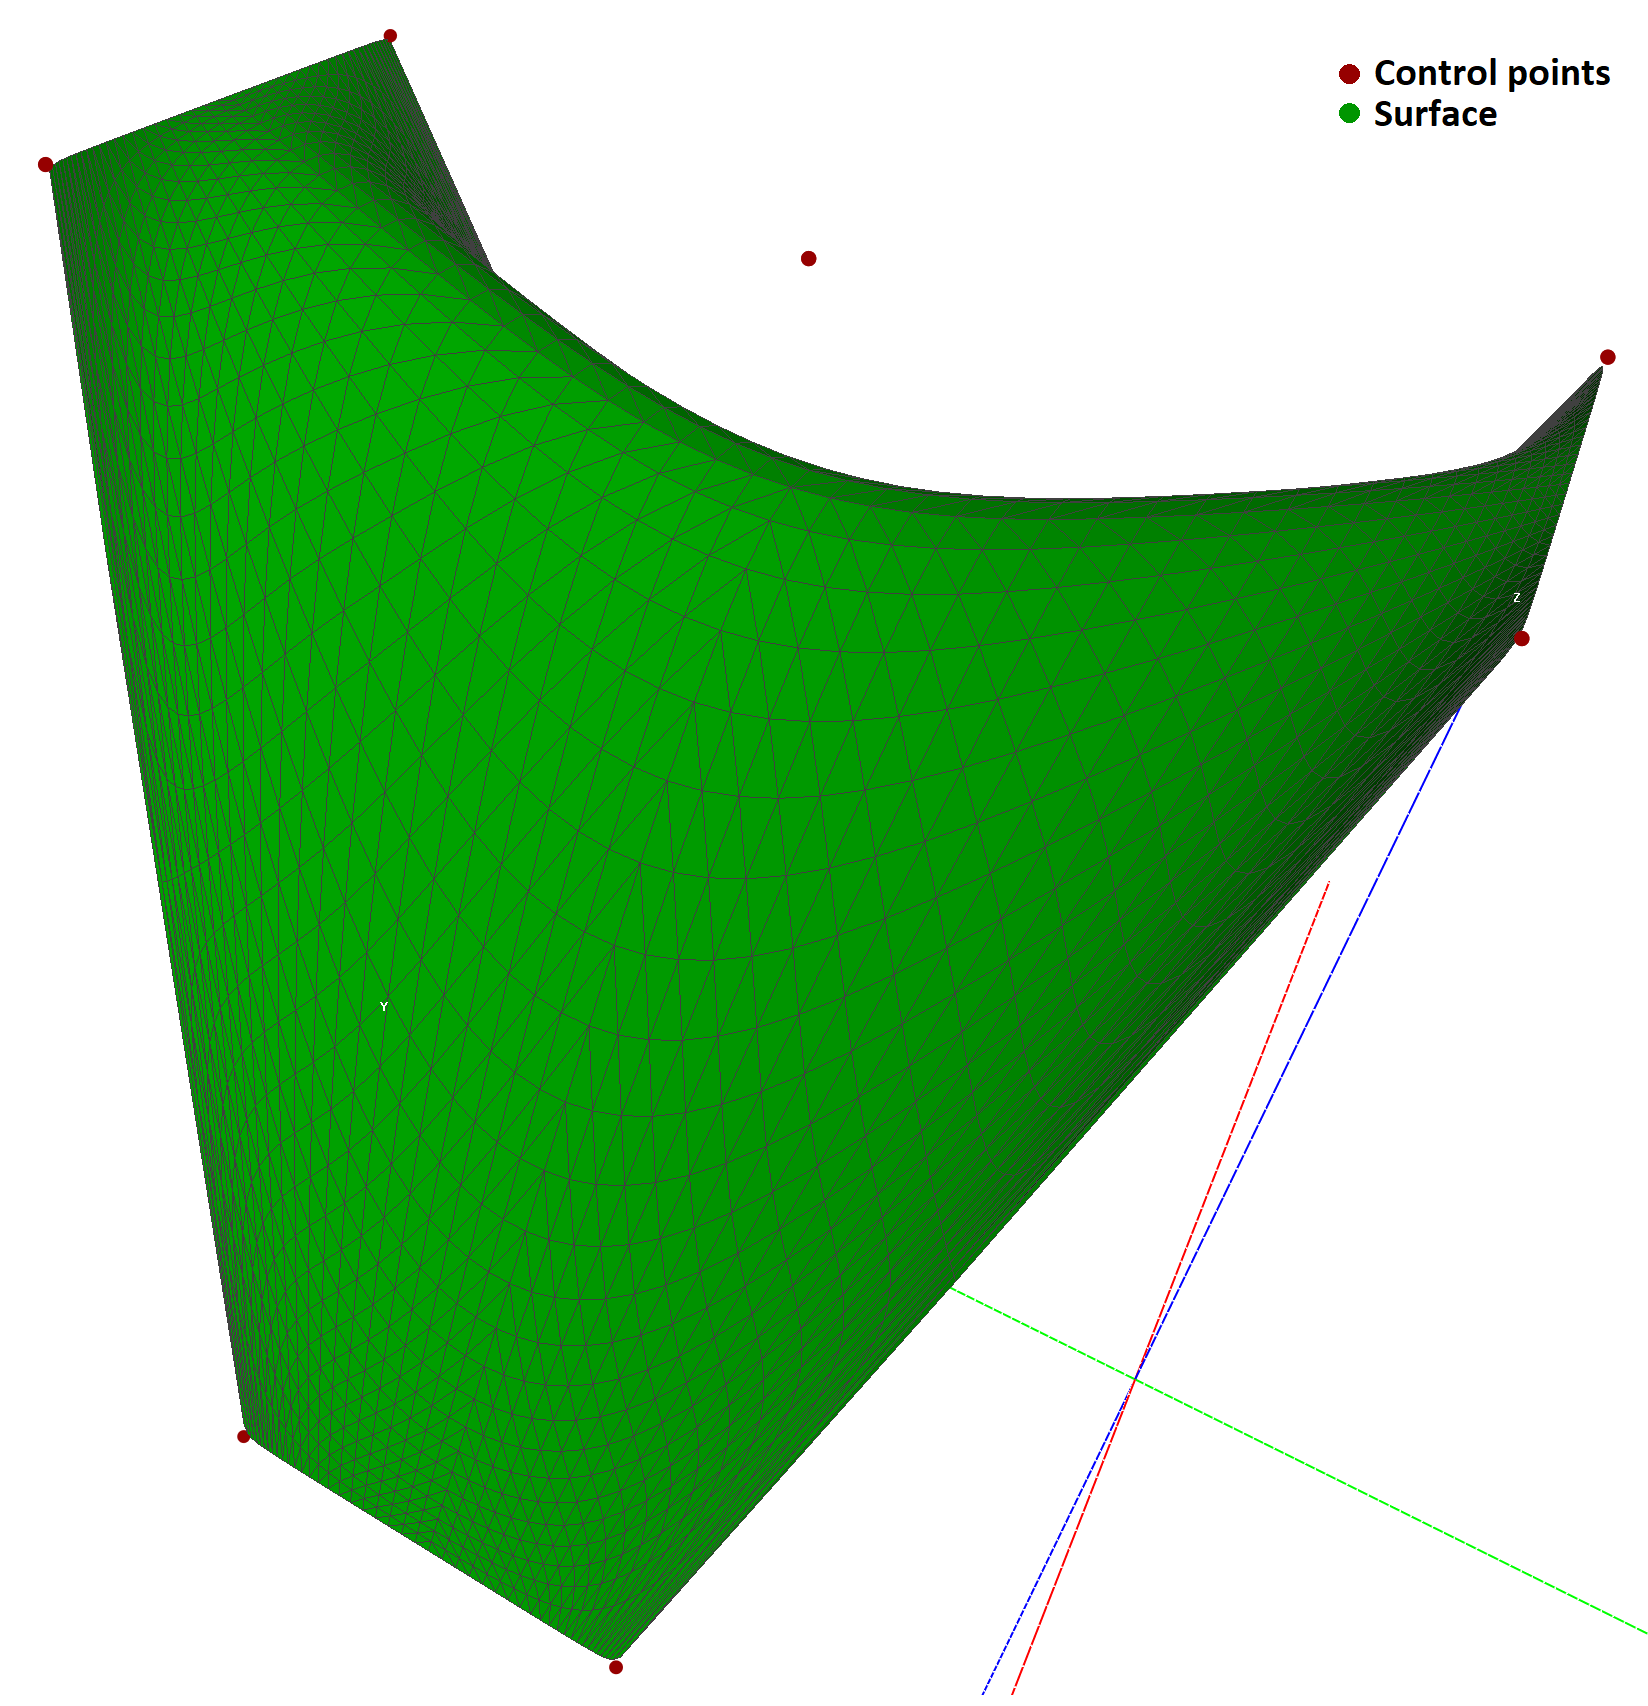
\includegraphics[width=\textwidth]{saddle2b}
\caption{Smoother central part in \texttt{saddle2b}.}
\label{saddle2b}
\end{subfigure}
\caption{T-spline surfaces of \texttt{saddle2}. Flatter saddle shape in the middle after knot shift.}
\label{saddle2}
\end{figure}

\subsection{Knot change along border off the grid}

\vspace{6pt}

In this section, let us start with \texttt{saddle3a} at the following setup: $T_{0, d}$ = $T_{1, d}$ in case of control points closer to the lower end of a border, and $T_{3, d}$ = $T_{4, d}$ in case of control points closer to the higher end of a border, and $d$ represents the appropriate dimension along which the corresponding border lies. So for example: $t_{2, 0, 1}$ = $t_{2, 1, 1}$ (red in Figure \ref{saddle3p}), and $t_{8, 3, 2}$ = $t_{8, 4, 2}$ (blue in Figure \ref{saddle3p}).

\begin{figure}[H]
\centering
\begin{subfigure}[b]{0.31\textwidth}
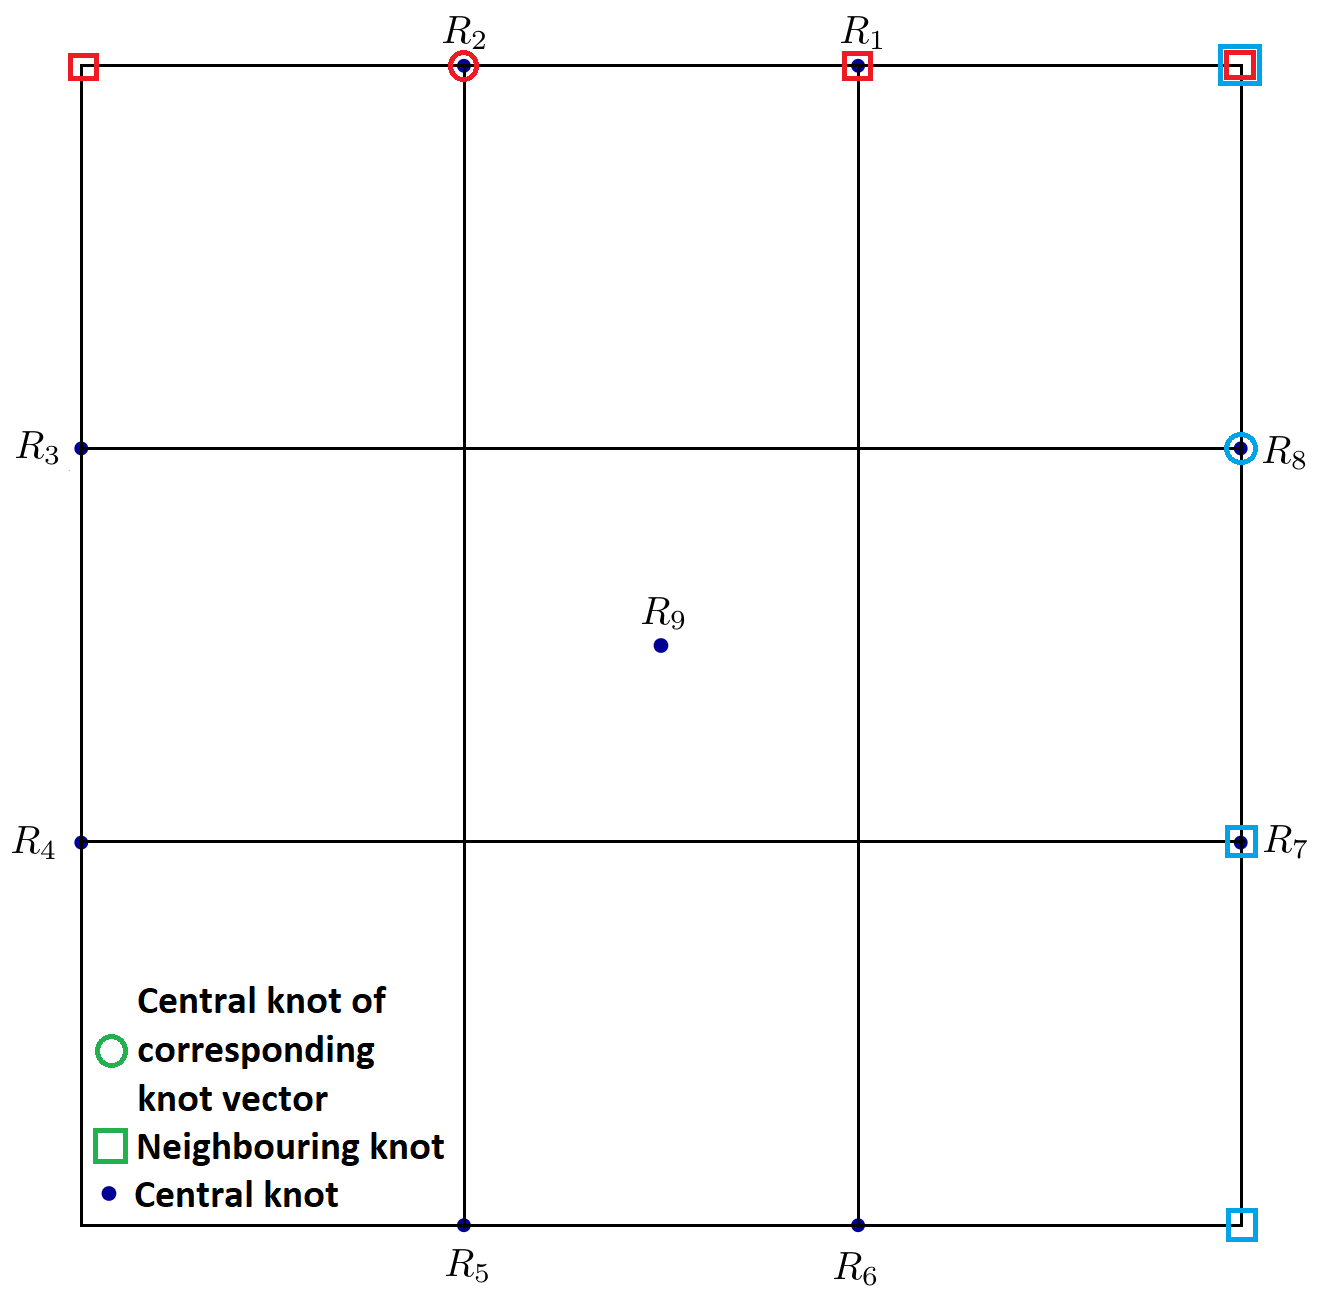
\includegraphics[width=\textwidth]{saddle3aparam}
\caption{Parametric space of \texttt{saddle3a} with knot vectors distributed across the grid.}
\label{saddle3ap}
\end{subfigure}
\begin{subfigure}[b]{0.31\textwidth}
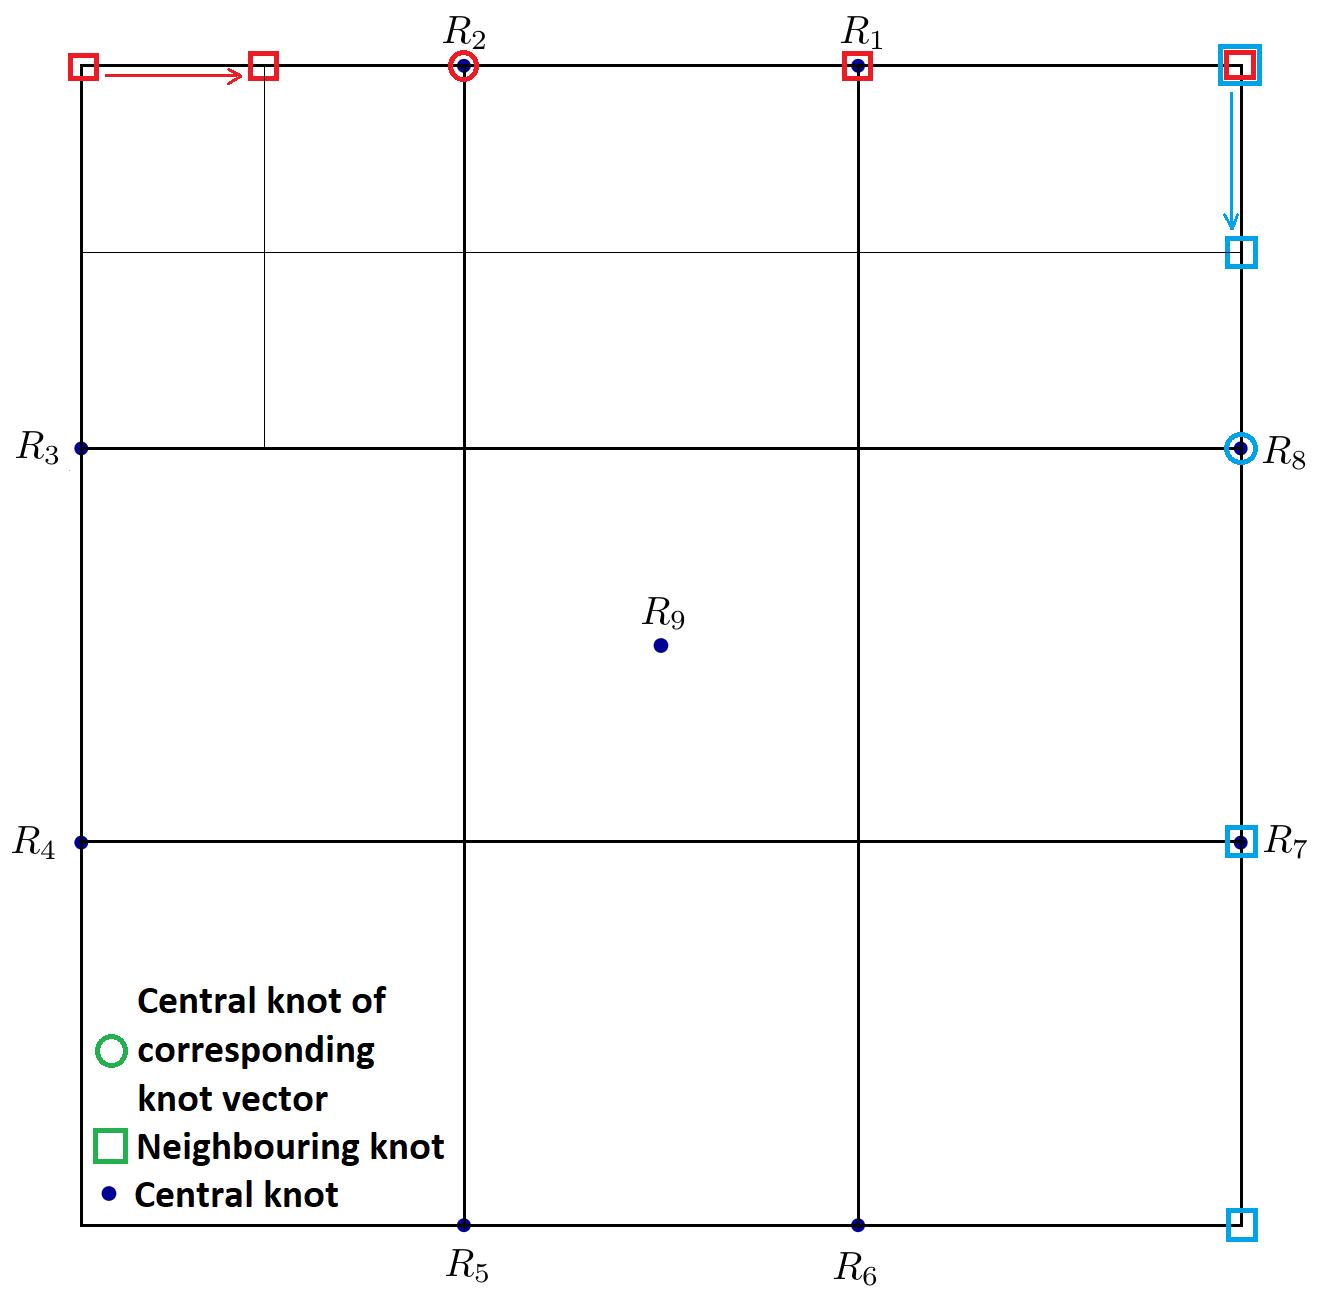
\includegraphics[width=\textwidth]{saddle3bparam}
\caption{Parametric space of \texttt{saddle3b} with change in duplicated knots inwards the border dimension.}
\label{saddle3bp}
\end{subfigure}
\begin{subfigure}[b]{0.34\textwidth}
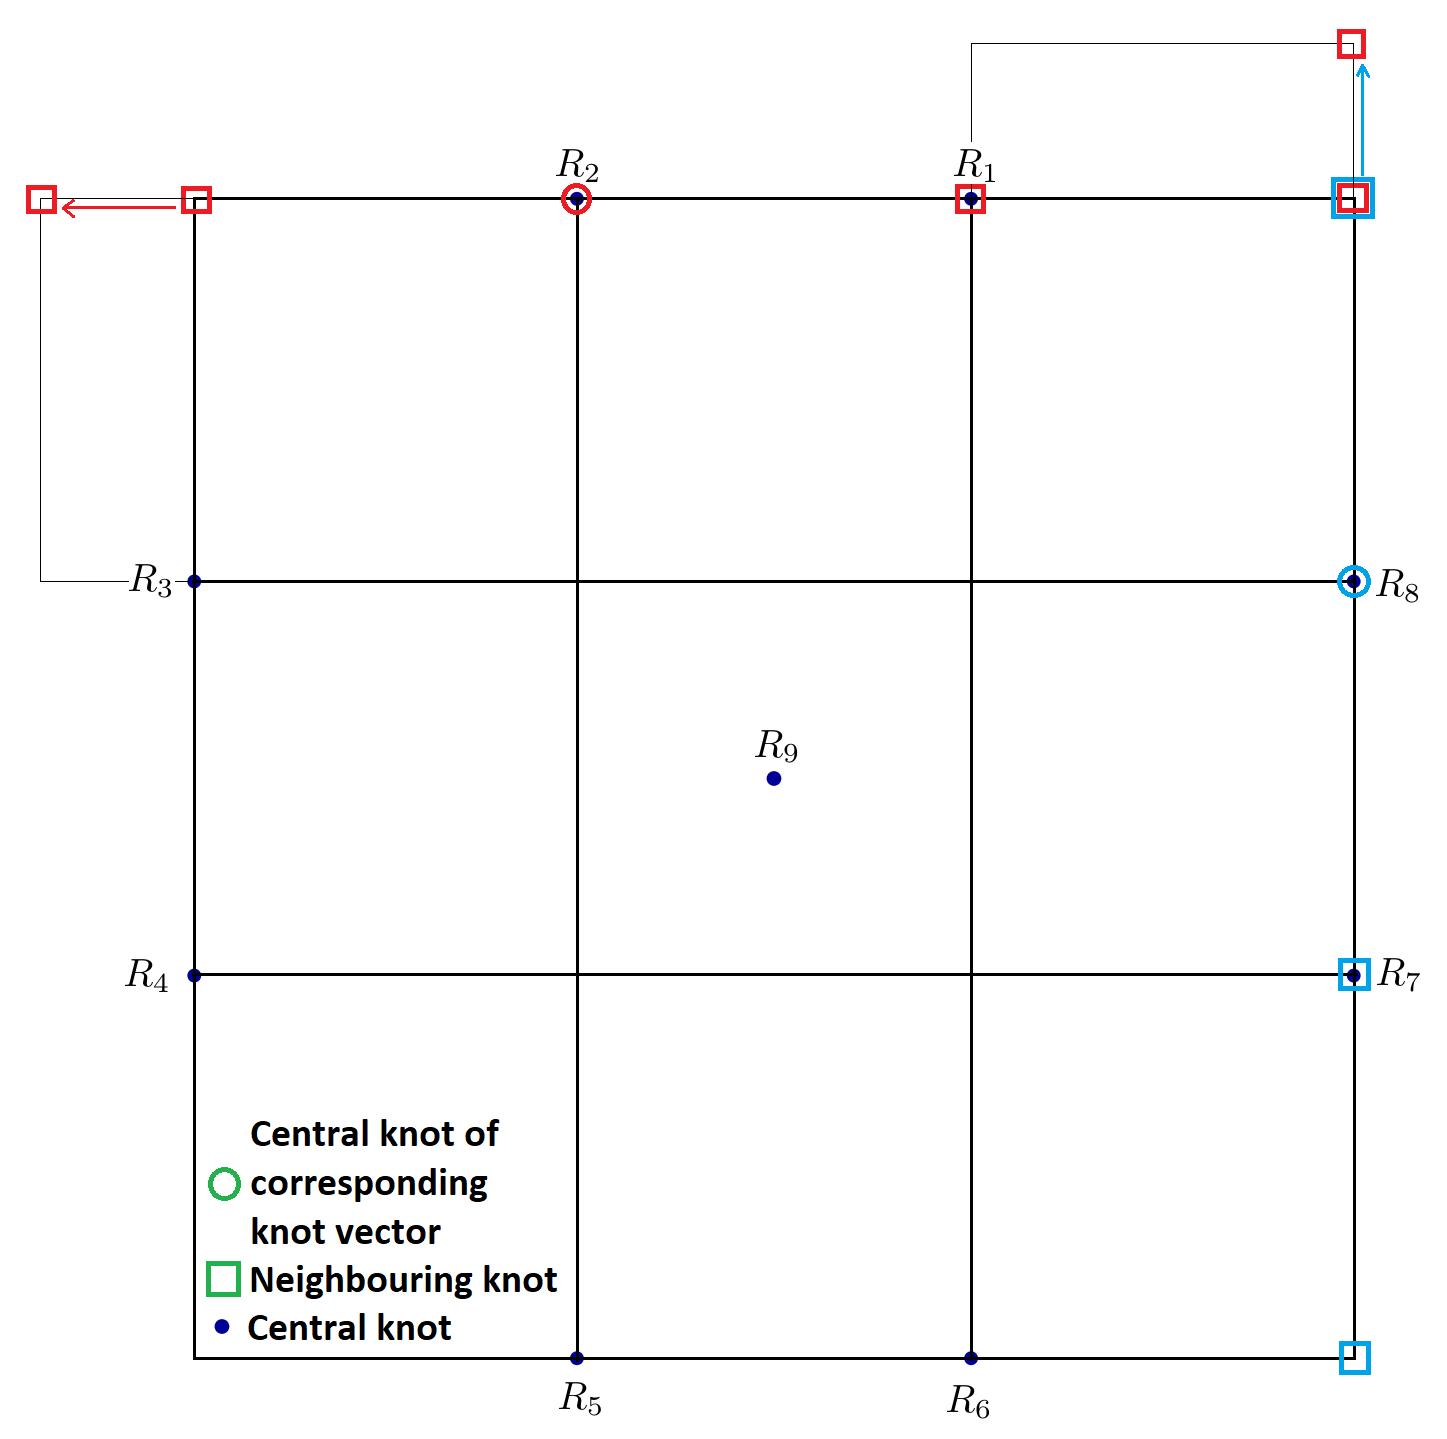
\includegraphics[width=\textwidth]{saddle3cparam}
\caption{Parametric space of \texttt{saddle3c} with change in duplicated knots outwards the border dimension.}
\label{saddle3cp}
\end{subfigure}
\caption{Parametric space of each surface with two examples (red and blue).}
\label{saddle3p}
\end{figure}

In \texttt{saddle3a} the setup is the same as in \texttt{saddle1a} or \texttt{saddle2a}. The are border knot coordinates - as it was mentioned above - that are equal. This will be changed in \texttt{saddle3b}. The red and blue examples are as follows:

\begin{equation}
\begin{split}
t_{2, 0, 1} & = 0 \phantom{0.15wwwww} t_{8, 3, 2} = 0.85 \\
t_{2, 1, 1} & = 0.15 \phantom{0wwwww} t_{8, 4, 2} = 1
\end{split}
\end{equation}

The "problem" with that is there is no central knot associated with 0.15 and 0.85. $t_{2, 0}$ = $t_{1, 0}$, so the secondary AOE between $T_{0}$ and $T_{1}$ is the same, having the same effect on the surface without extra control point. That will result in a "cut". This is essentially different from the \texttt{saddle1} example due to the lack of junction in the T-mesh. The reader is advised to take a closer look at \texttt{saddle1b} and \texttt{saddle3b}.

In \texttt{saddle3c}, knot vectors leave the [0,1] parametric space, but the surface is still generated on that area only. Therefore, the result is quite strange. I thought it might be helpful to illustrate the importance of right range. In order to get the full picture of how a T-spline surface looks, the variables along the whole parametric surface should be substituted.

\begin{figure}[H]
\centering
\begin{subfigure}[b]{0.32\textwidth}
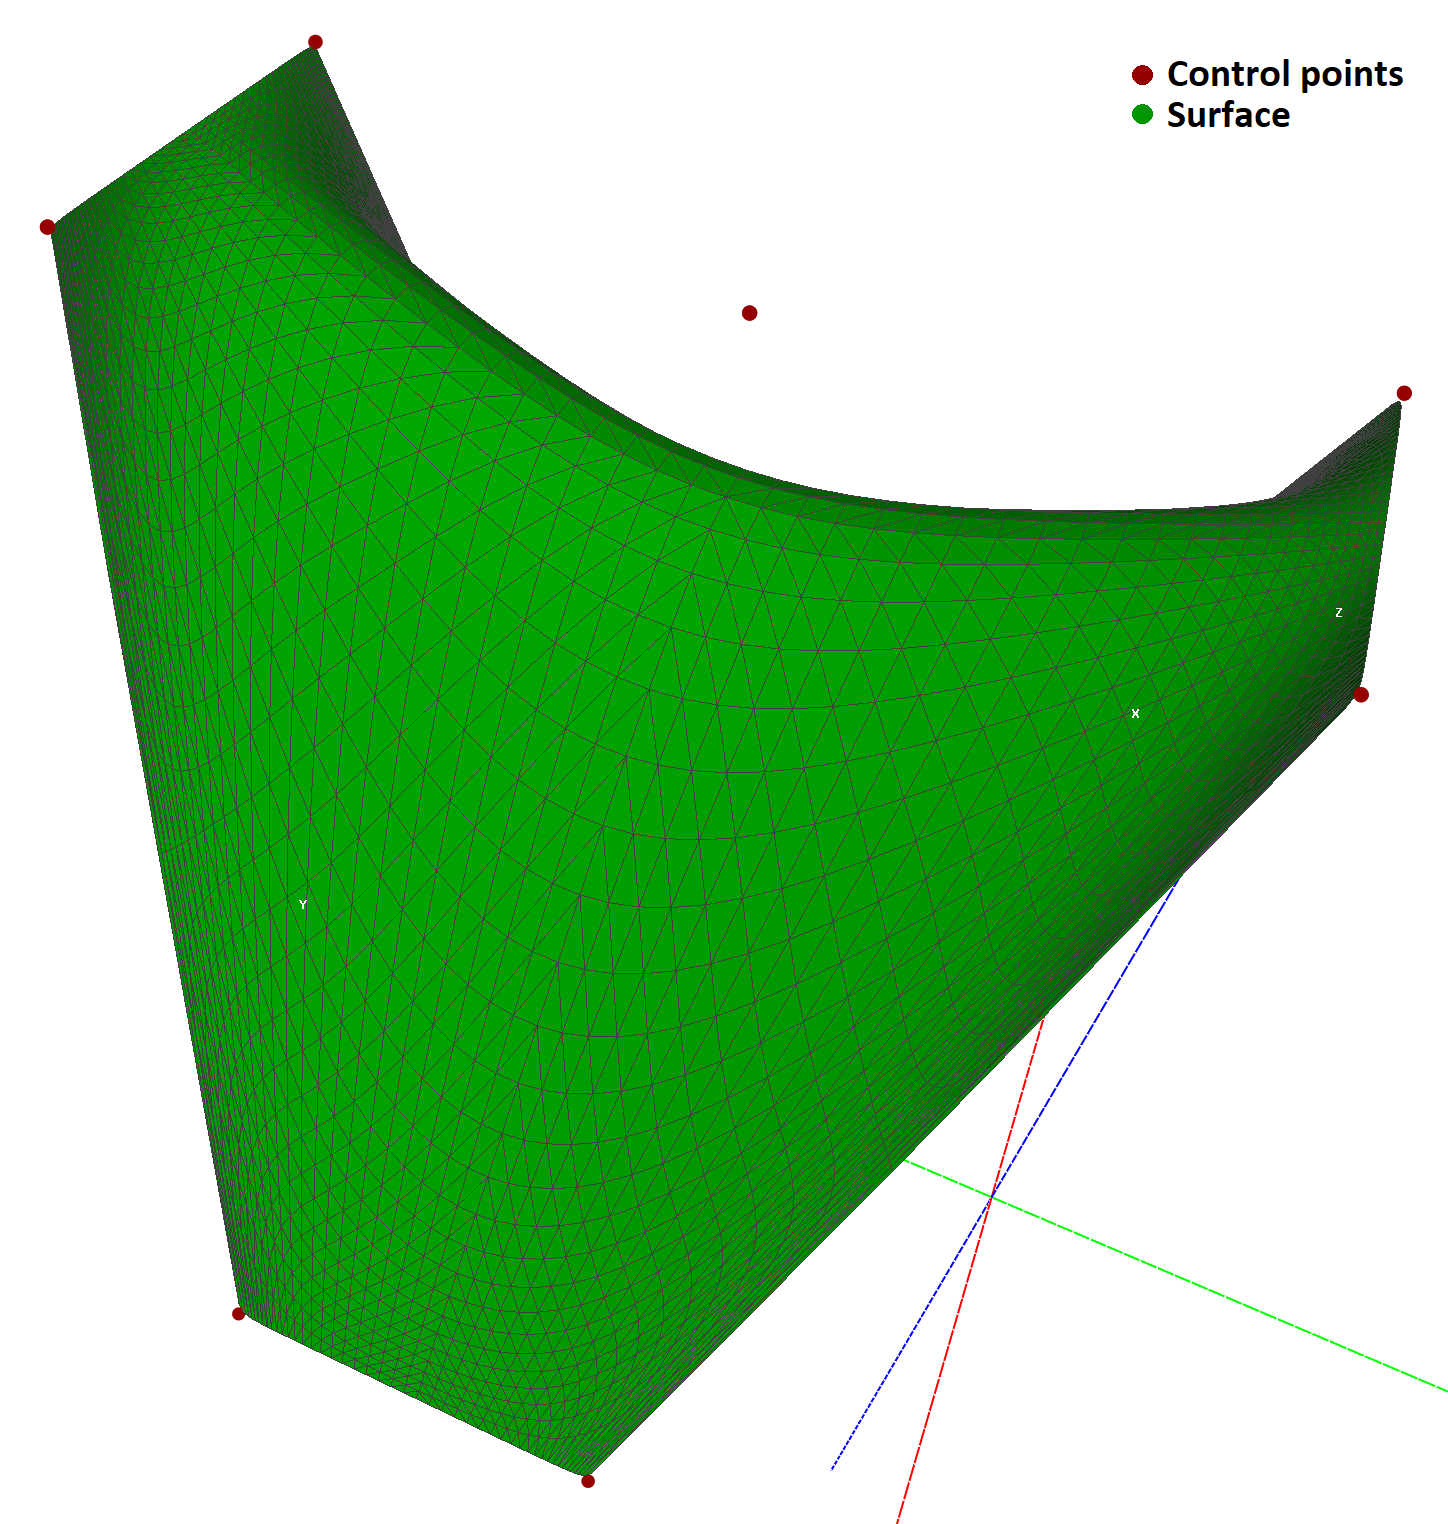
\includegraphics[width=\textwidth]{saddle3a}
\caption{Surface with duplicated knots.}
\label{saddle3a}
\end{subfigure}
\begin{subfigure}[b]{0.32\textwidth}
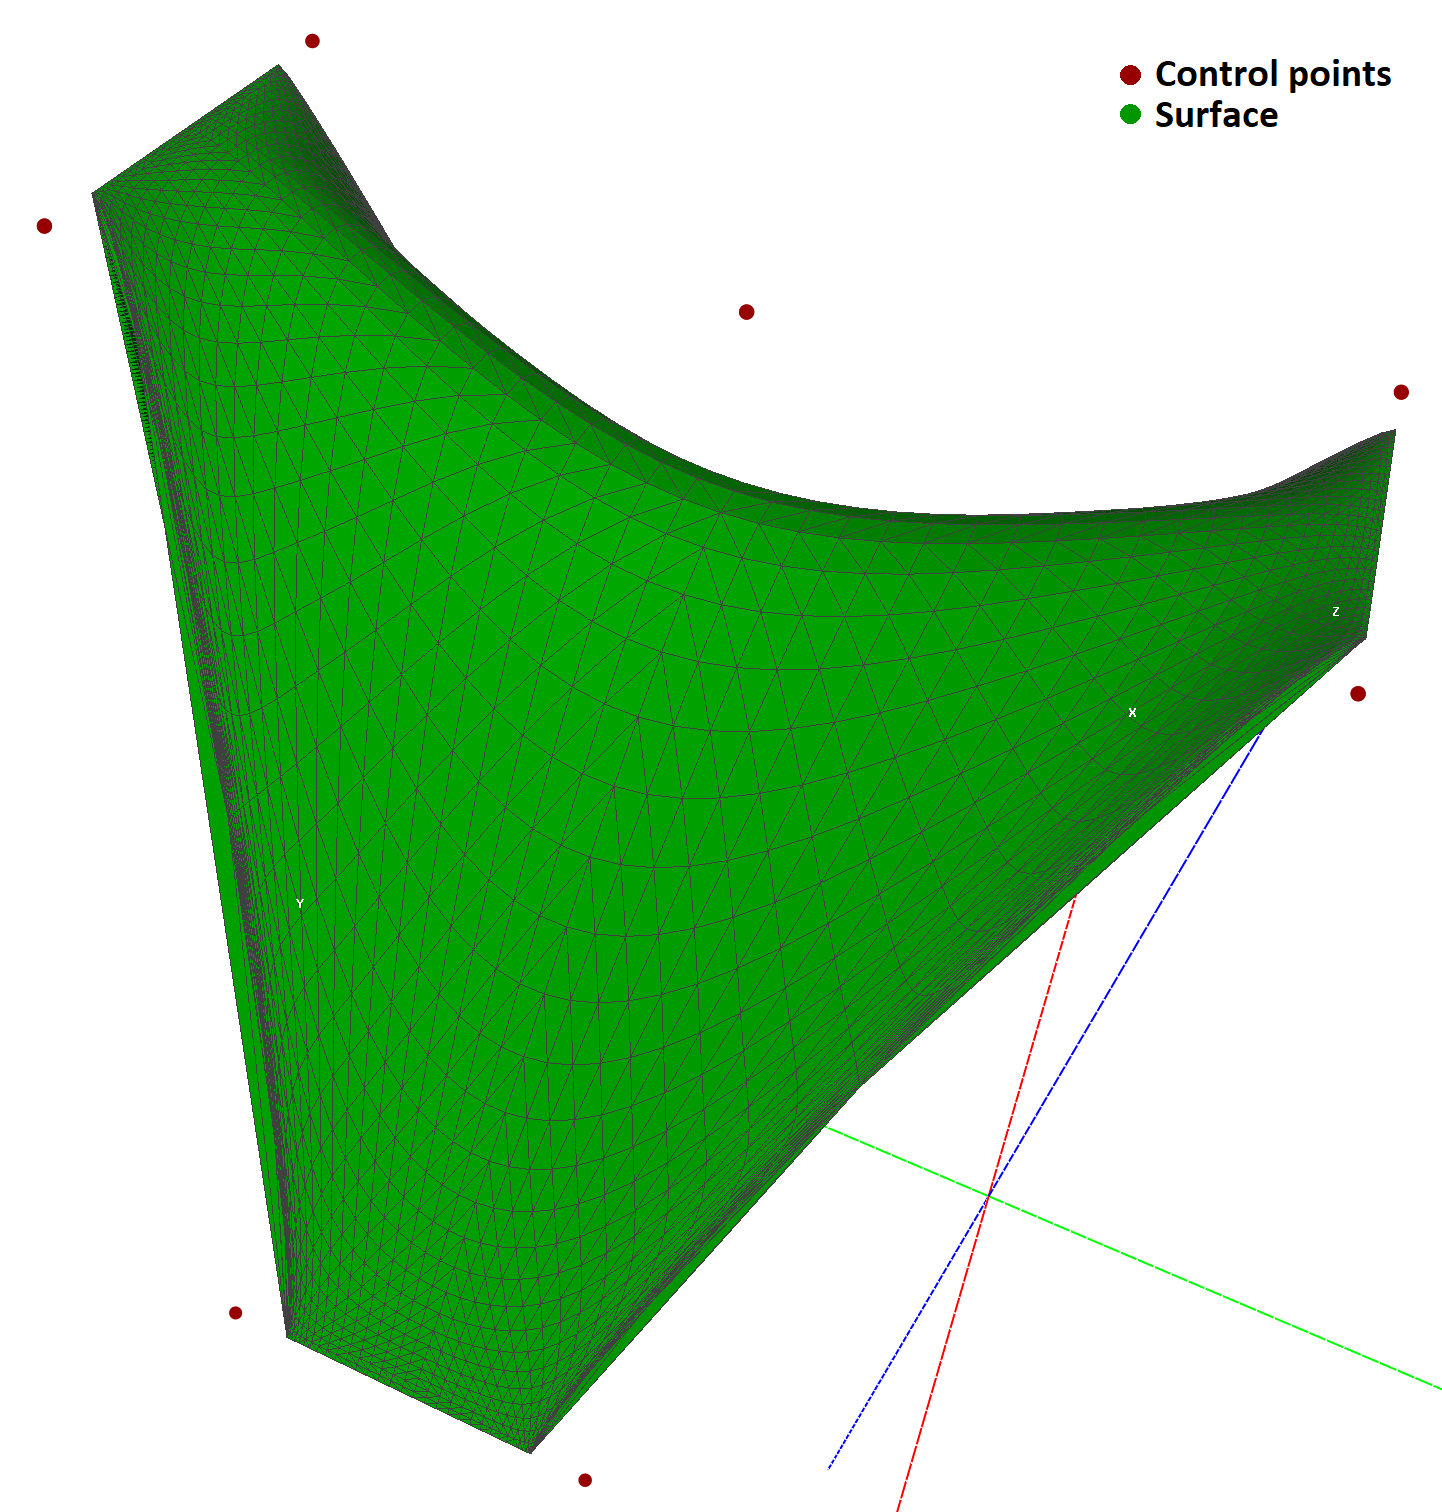
\includegraphics[width=\textwidth]{saddle3b}
\caption{Off grid surface.}
\label{saddle3b}
\end{subfigure}
\begin{subfigure}[b]{0.32\textwidth}
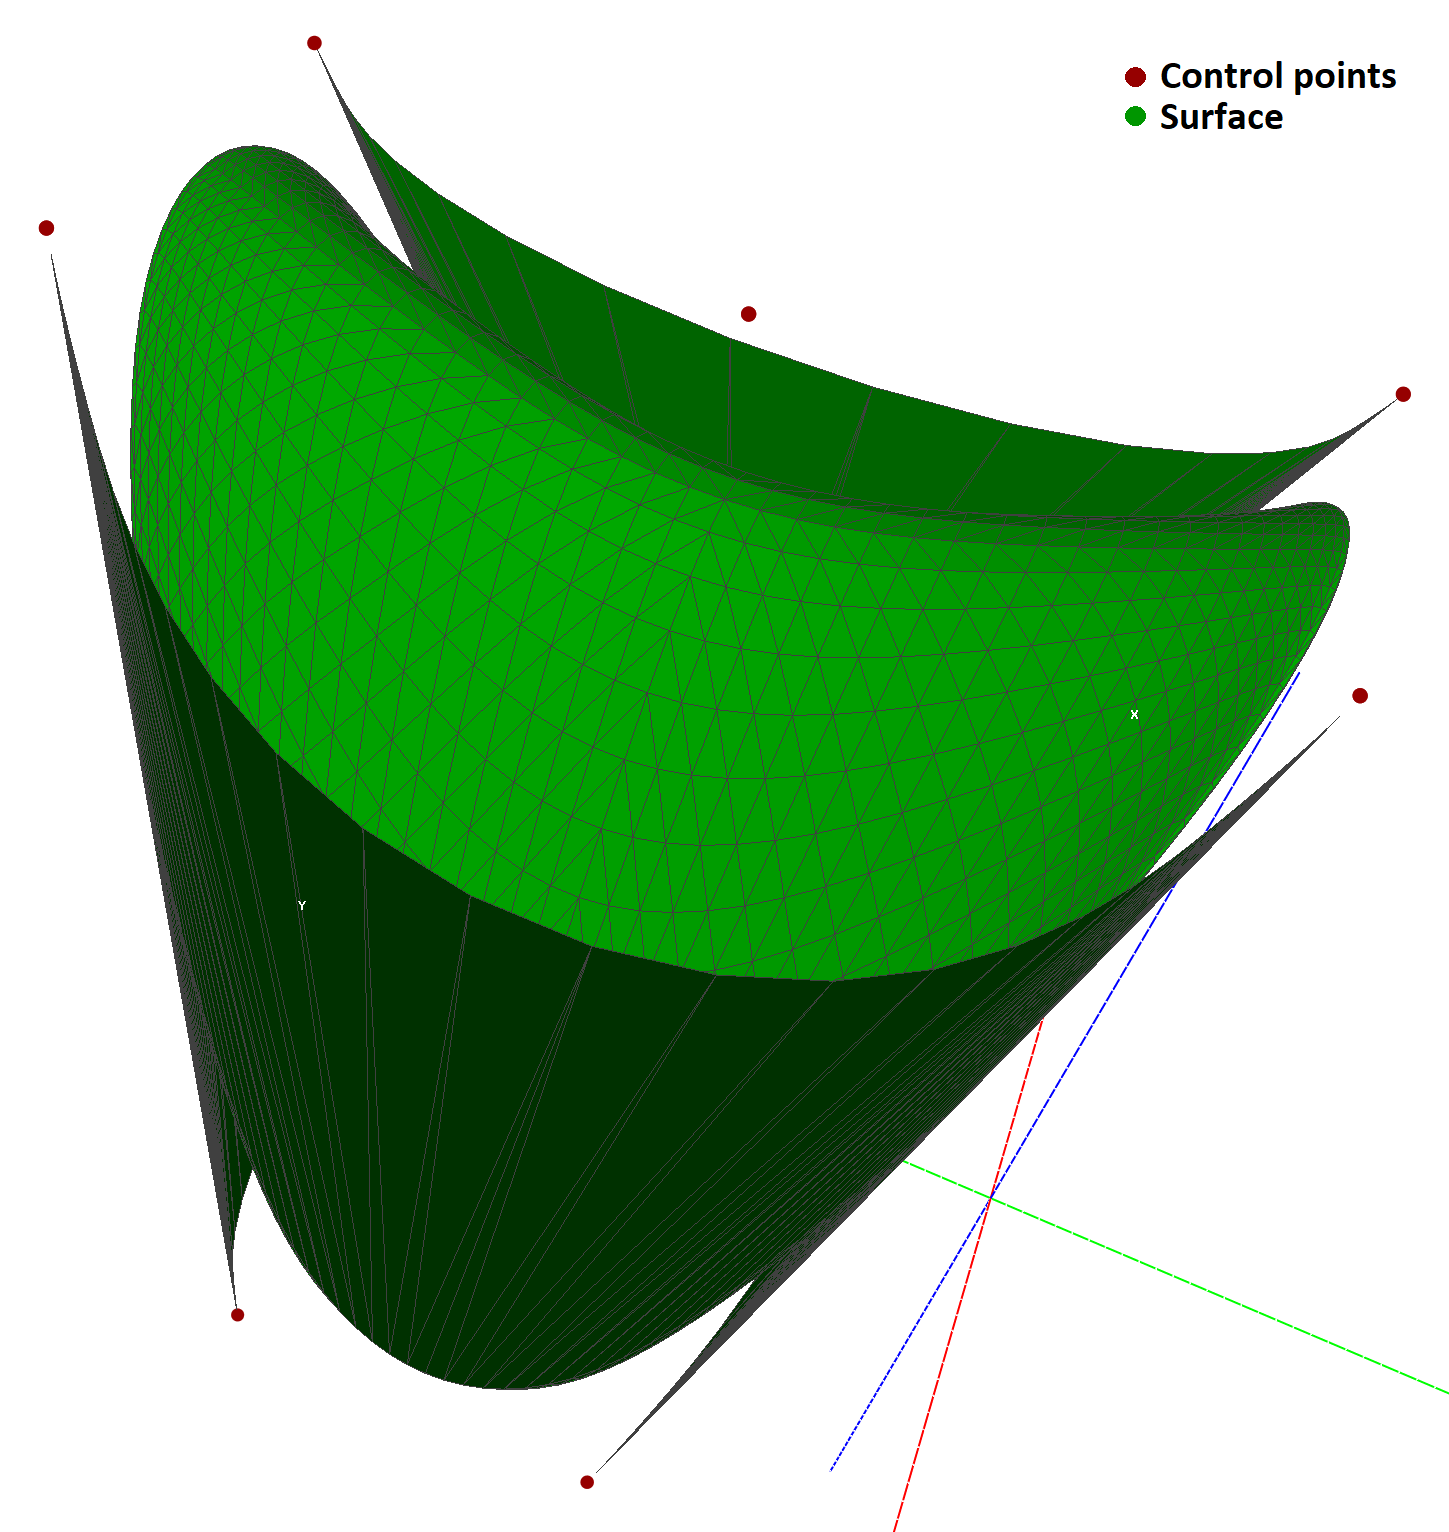
\includegraphics[width=\textwidth]{saddle3c}
\caption{Out of range surface.}
\label{saddle3c}
\end{subfigure}
\caption{T-spline surfaces of \texttt{saddle3}.}
\label{saddle3}
\end{figure}

\subsection{Local refinement inside surface}

\vspace{6pt}

Let us talk about local refinement now. Local refinement means that the surface is \emph{refined}, changed in a local space on the surface. In \texttt{saddle4a} only $R_1$, ..., $R_8$ control points are used, and $R_9$ will be added to the surface later. The knot vector of $R_9$ in \texttt{saddle4b} and \texttt{saddle4c} is shown in Equation \ref{knotsaddle4}.

\begin{equation}
\begin{split}
\texttt{saddle4b}: \phantom{ww} & t_{9} = ([0, 0.4], [0.2, 0.45], [0.5, 0.5], [0.8, 0.55], [1, 0.6]) \\
\texttt{saddle4c}: \phantom{ww} & t_{9} = ([0.4, 0], [0.45, 0.2], [0.5, 0.5], [0.55, 0.8], [0.6, 1])
\end{split}
\label{knotsaddle4}
\end{equation}

\begin{figure}[H]
\centering
\begin{subfigure}[b]{0.32\textwidth}
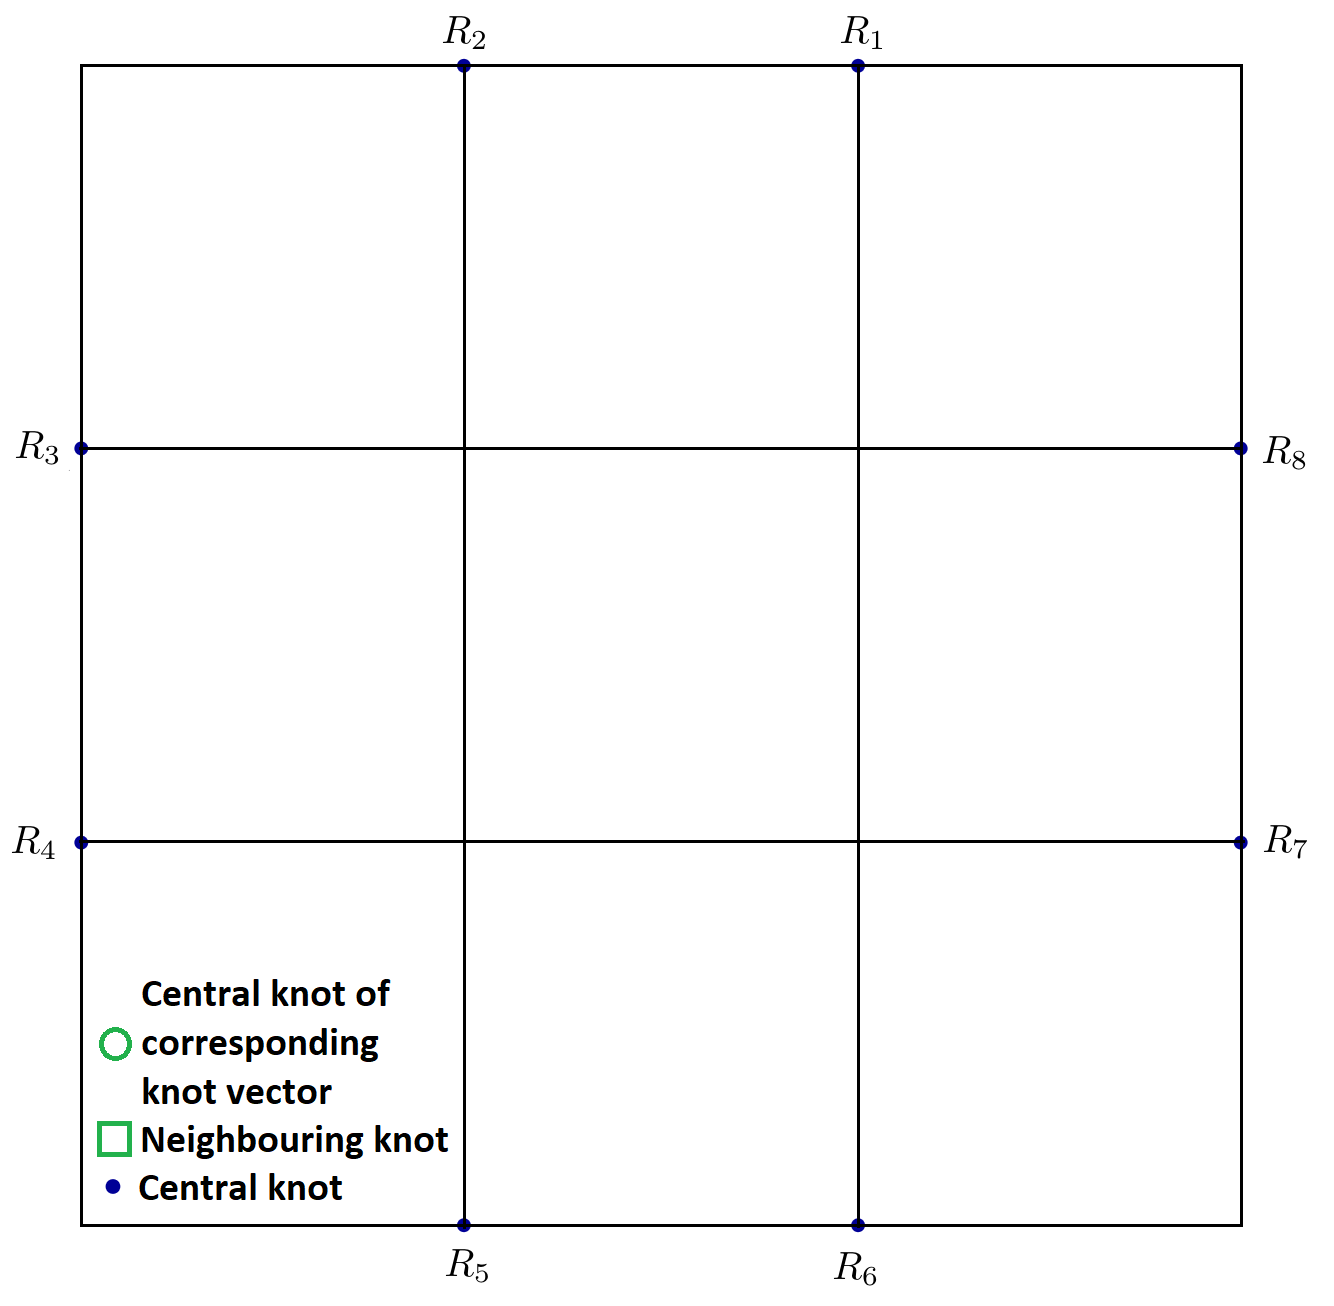
\includegraphics[width=\textwidth]{saddle4aparam}
\caption{Without local refinement, \texttt{saddle4a}.}
\label{saddle4ap}
\end{subfigure}
\begin{subfigure}[b]{0.32\textwidth}
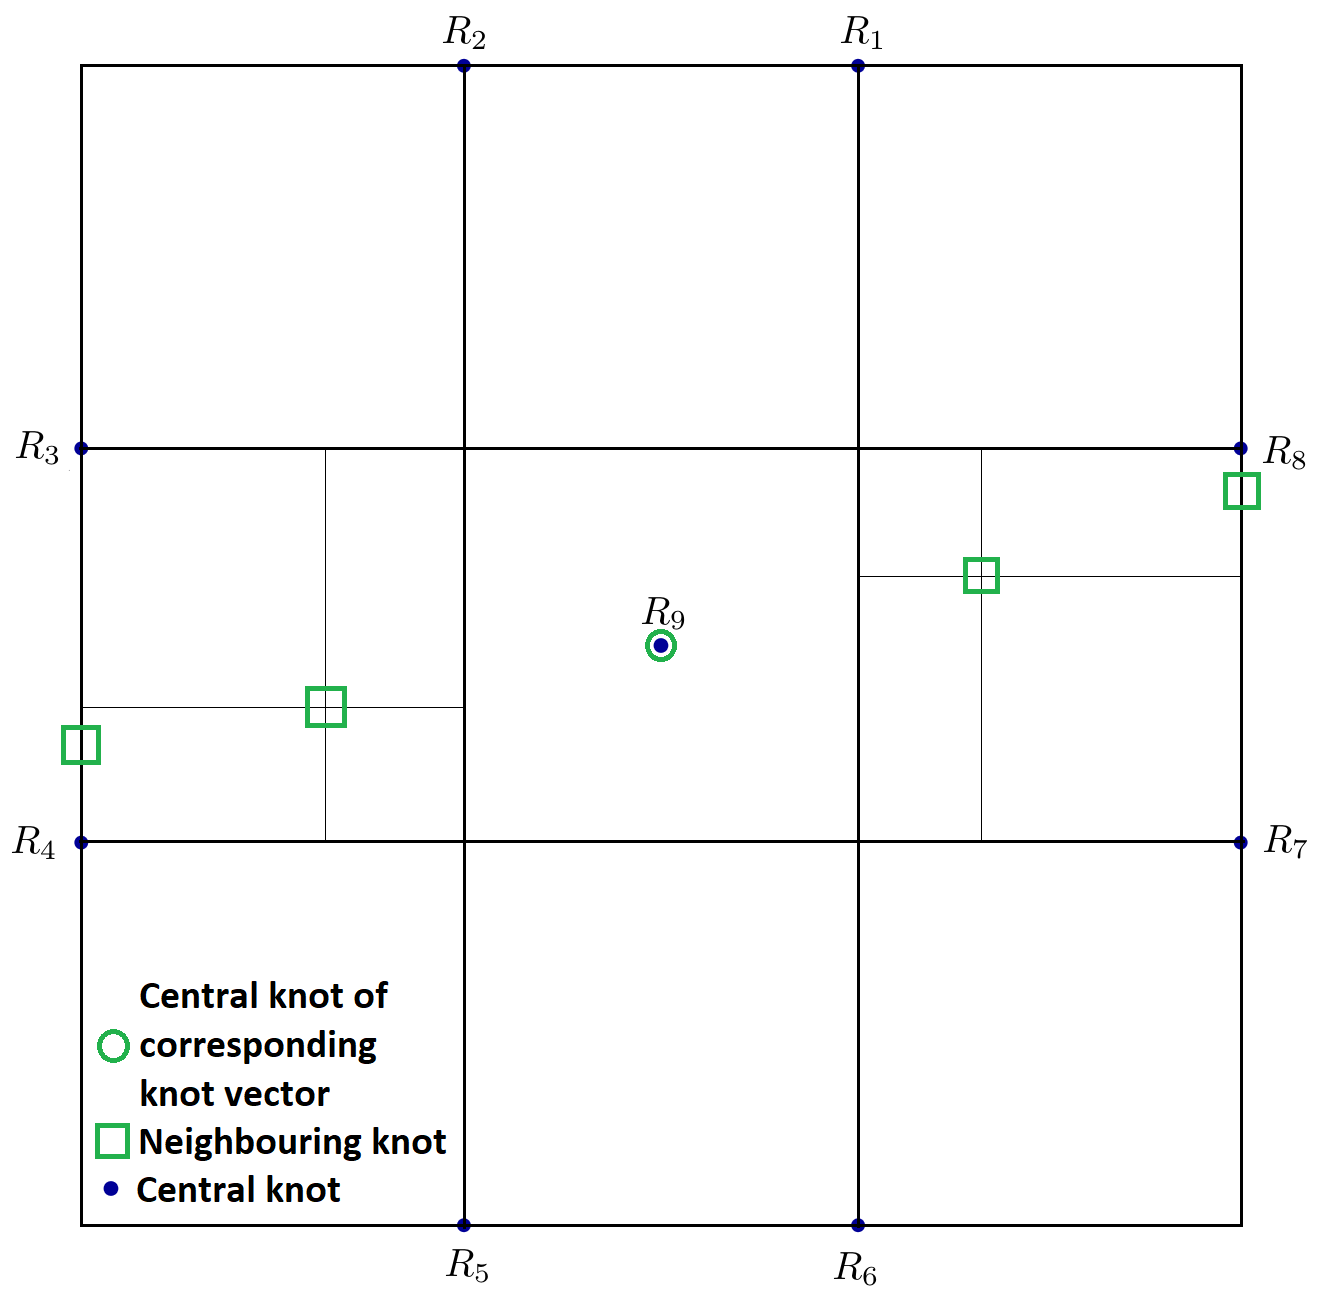
\includegraphics[width=\textwidth]{saddle4bparam}
\caption{Horizontally elongated local refinement, \texttt{saddle4b}.}
\label{saddle4bp}
\end{subfigure}
\begin{subfigure}[b]{0.32\textwidth}
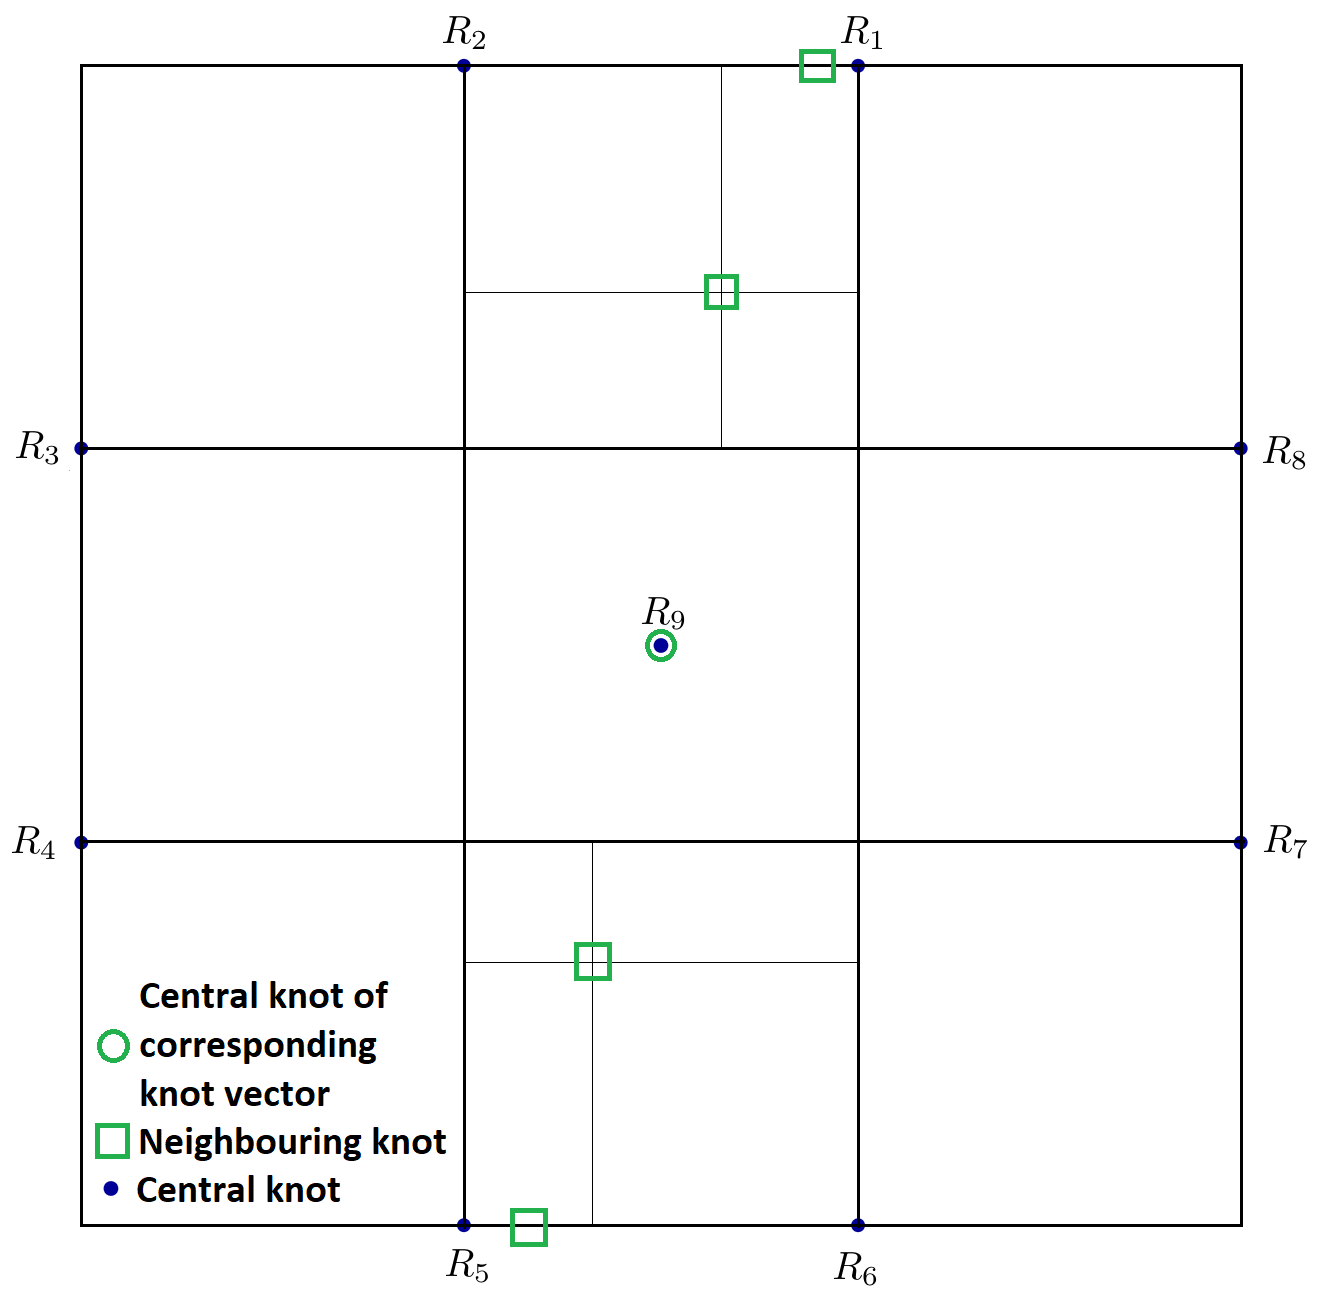
\includegraphics[width=\textwidth]{saddle4cparam}
\caption{Vertically elongated local refinement, \texttt{saddle4c}.}
\label{saddle4cp}
\end{subfigure}
\caption{Parametric space of \texttt{saddle4} surfaces.}
\label{saddle4p}
\end{figure}

In \texttt{saddle4b} the bump on the surface is elongated in the horizontal parametric dimension ($x$-axis in real space), in \texttt{saddle4c} it is elongated in the vertical parametric dimension ($y$-axis in real space). The explanation is simple: when a control point is more restricted in one dimension and less in the other, its AOE will be elongated. It is simply because over the restriction, the respective control point has no affect on the surface, so over that restriction, the surface remains as it was without the additional control point. This is shown in Figure \ref{saddle4}.

\begin{figure}[H]
\centering
\begin{subfigure}[b]{0.32\textwidth}
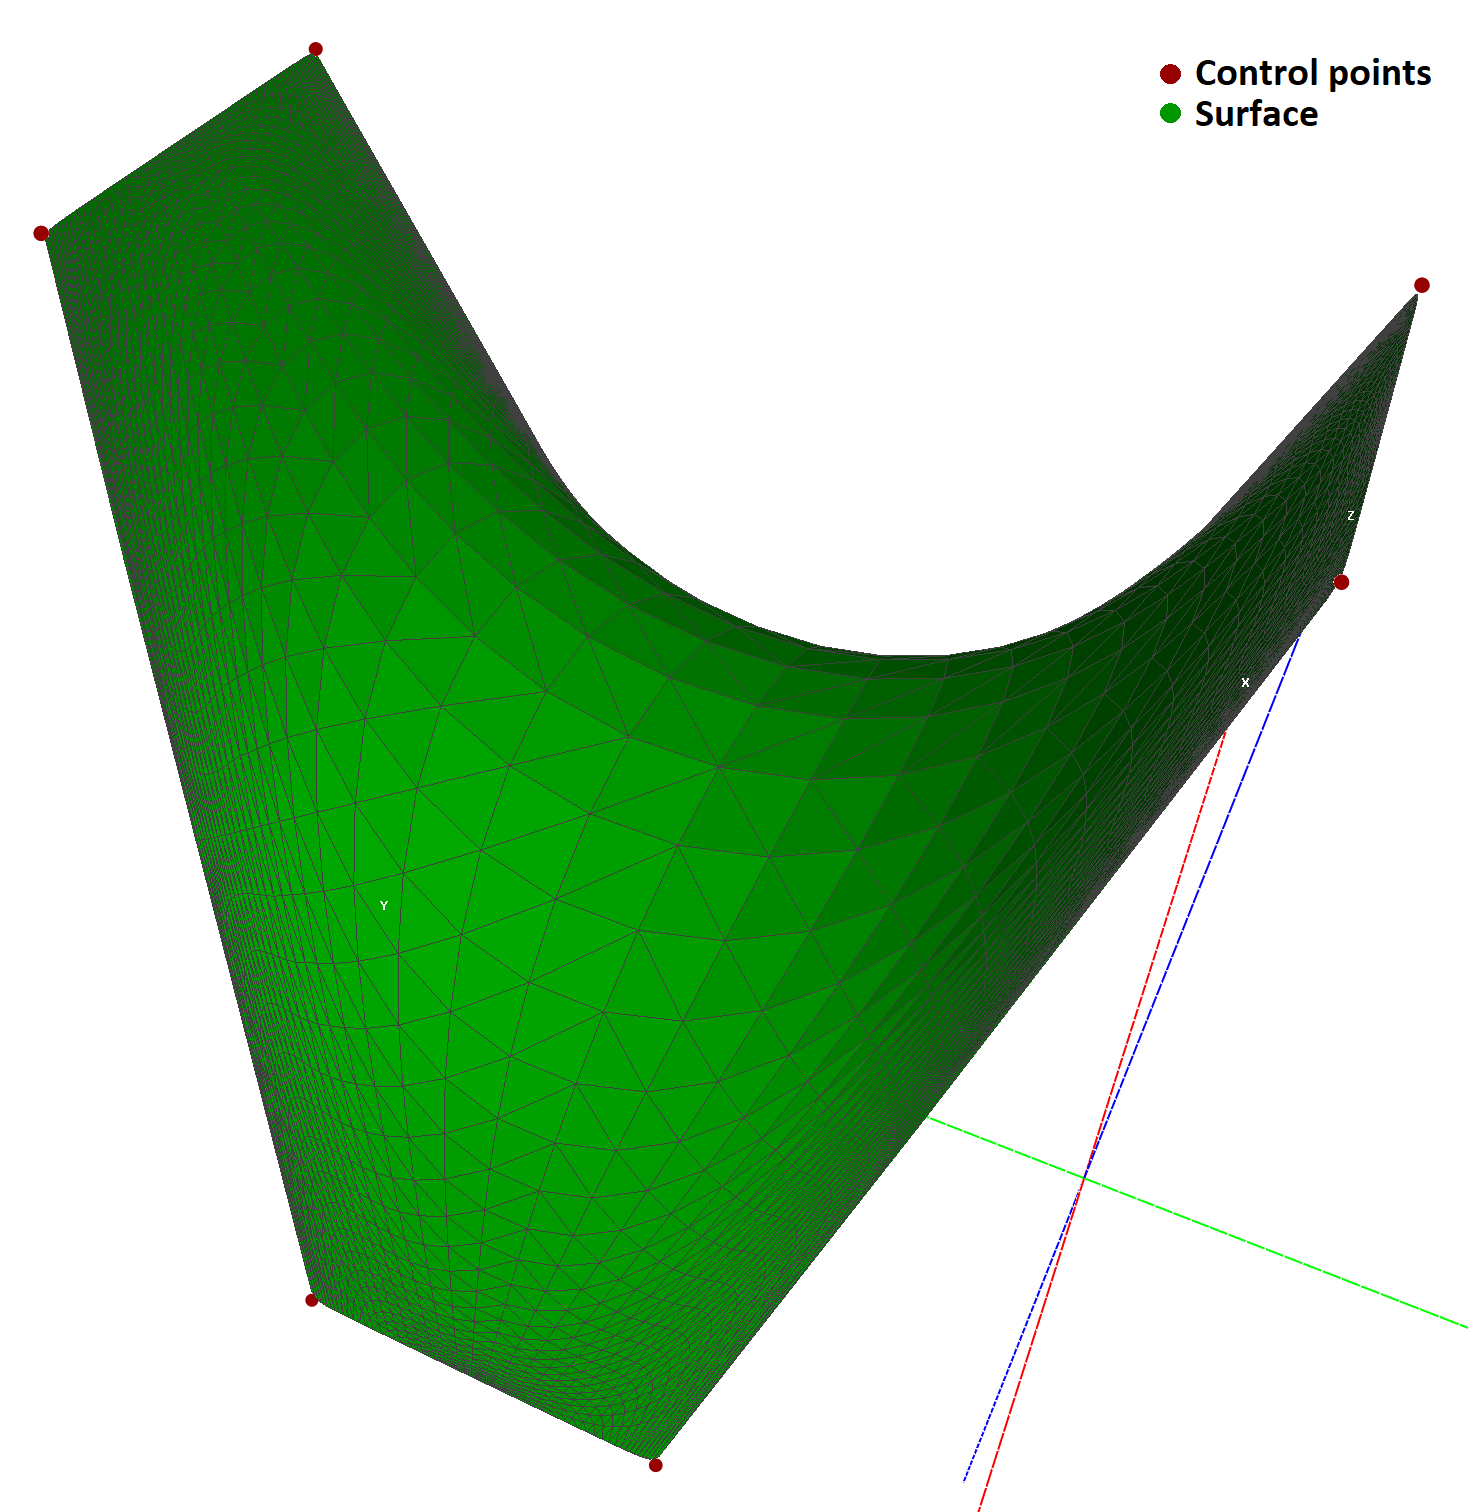
\includegraphics[width=\textwidth]{saddle4a}
\caption{Surface without $R_9$.}
\label{saddle4a}
\end{subfigure}
\begin{subfigure}[b]{0.32\textwidth}
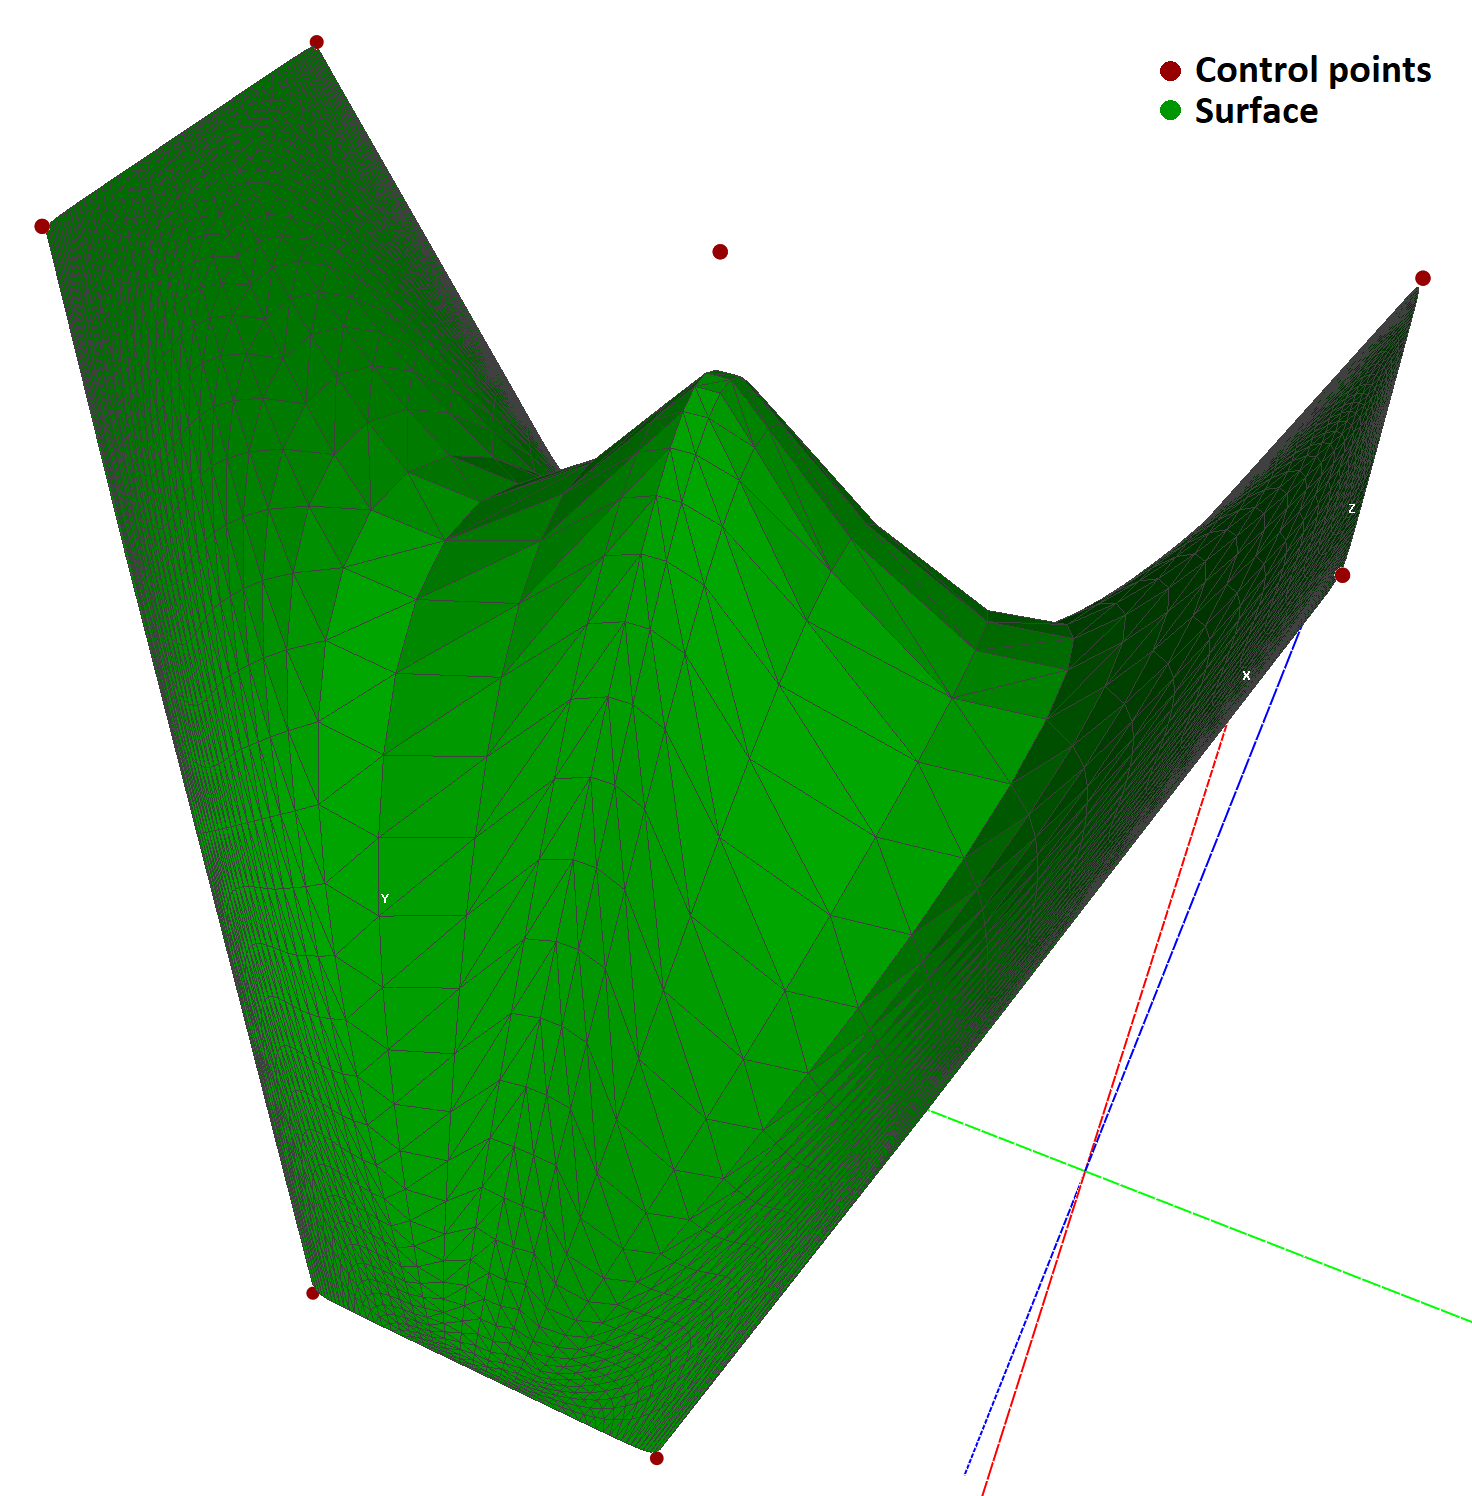
\includegraphics[width=\textwidth]{saddle4b}
\caption{$R_9$ with horizontal elongation.}
\label{saddle4b}
\end{subfigure}
\begin{subfigure}[b]{0.32\textwidth}
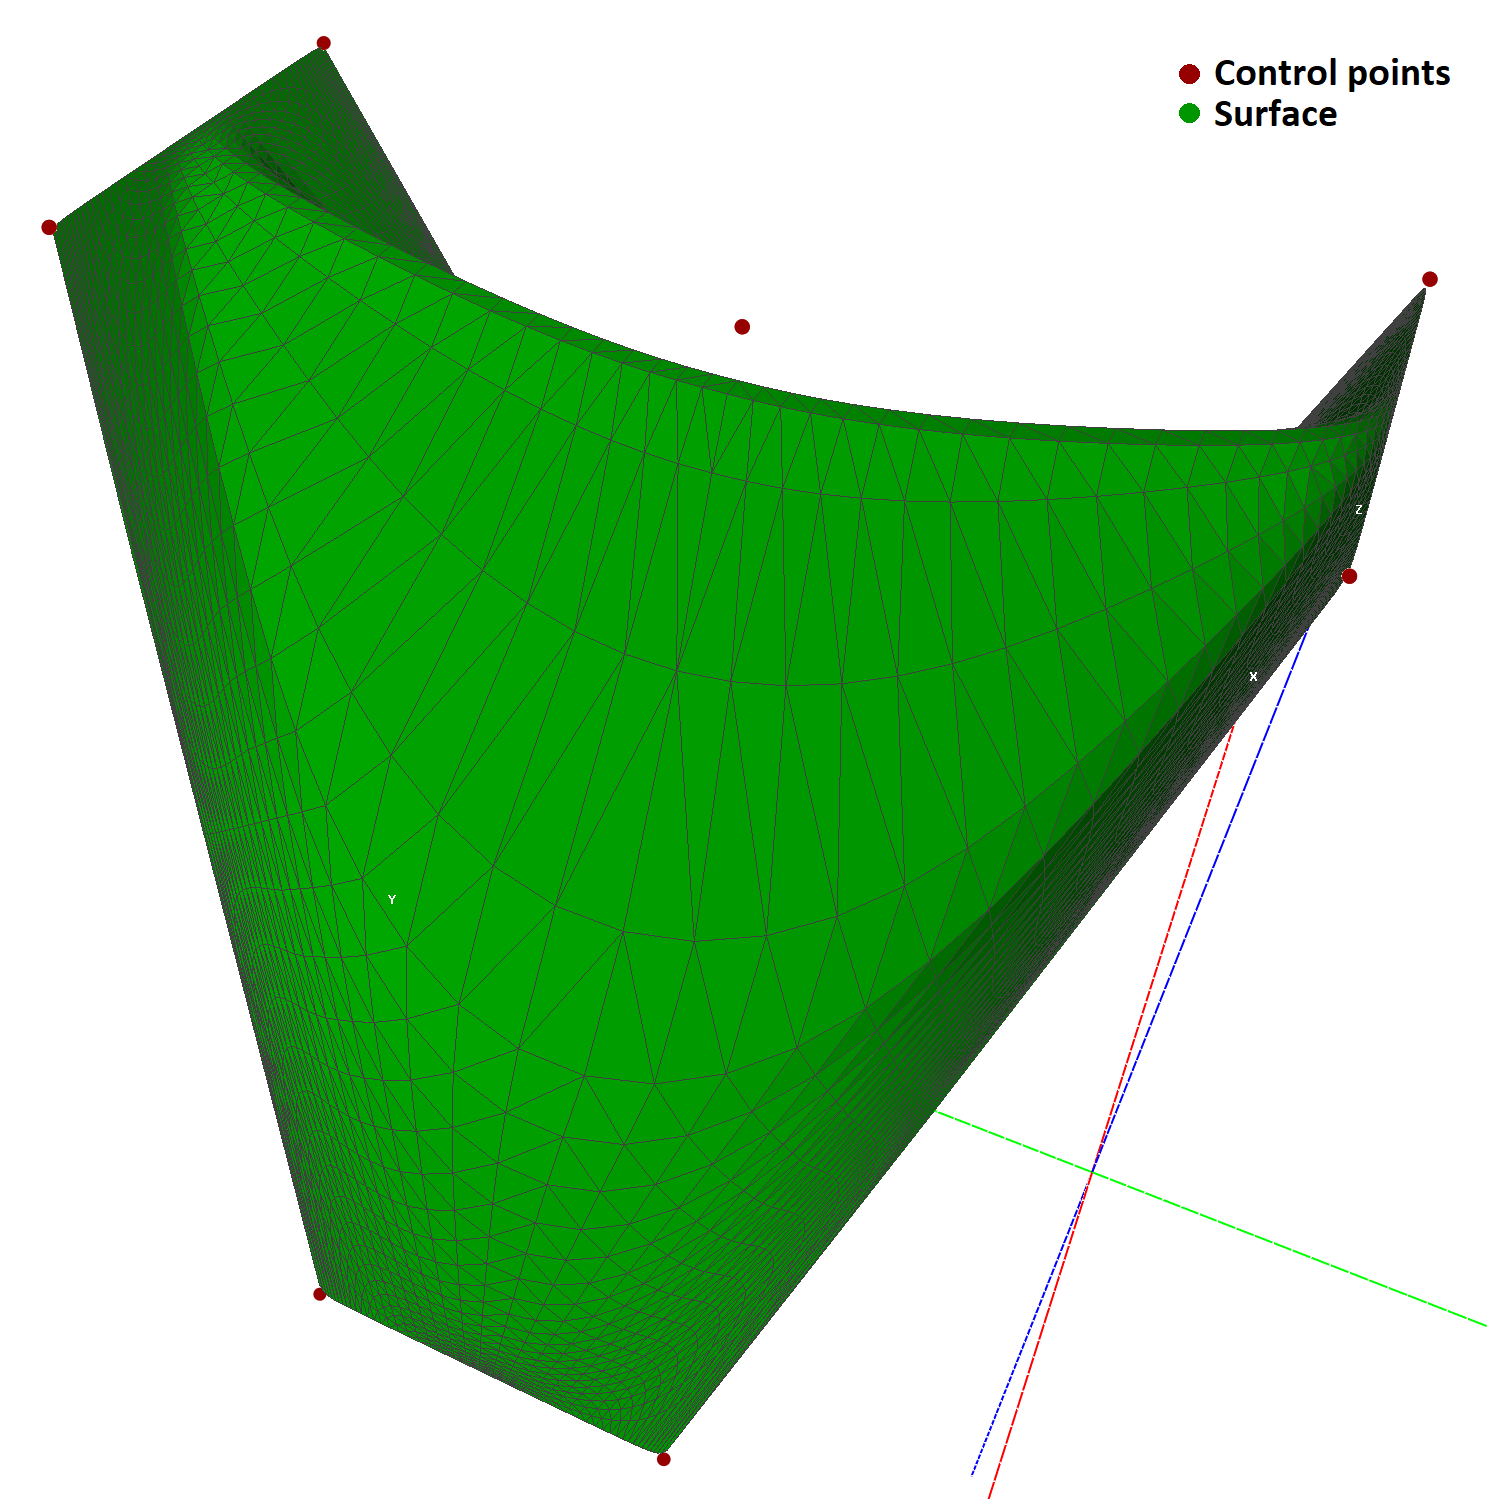
\includegraphics[width=\textwidth]{saddle4c}
\caption{$R_9$ with vertical elongation.}
\label{saddle4c}
\end{subfigure}
\caption{T-spline surfaces of \texttt{saddle4} with and without local refinement.}
\label{saddle4}
\end{figure}

\subsection{Local refinement along border}

\vspace{6pt}

The next example will be similar to the previous one, but in this case, the border will be locally refined. The same $R_9$ is used with the following knot vector:

\begin{equation}
t_{9} = ([0.33, 0], [0.33, 0], [0.5, 0], [0.67, 0.33], [0.67, 0.67])
\end{equation}

\begin{figure}[H]
\centering
\begin{subfigure}[b]{0.48\textwidth}
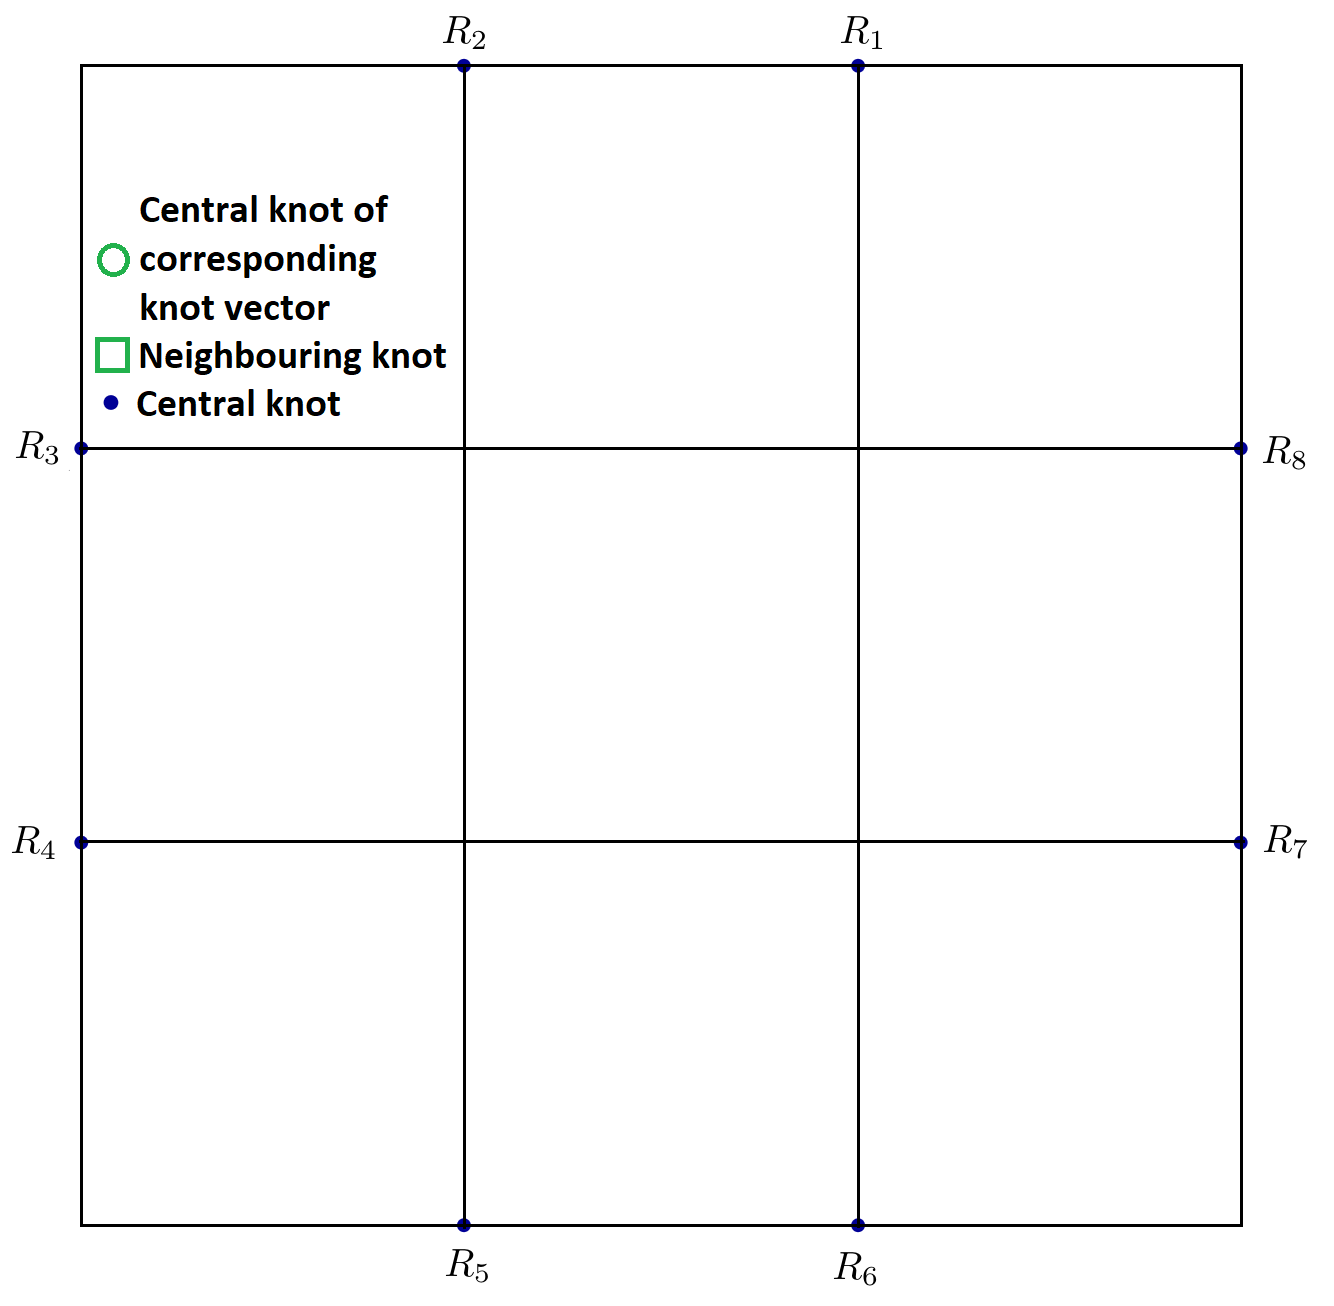
\includegraphics[width=\textwidth]{saddle5aparam}
\caption{}
\label{saddle5ap}
\end{subfigure}
\begin{subfigure}[b]{0.48\textwidth}
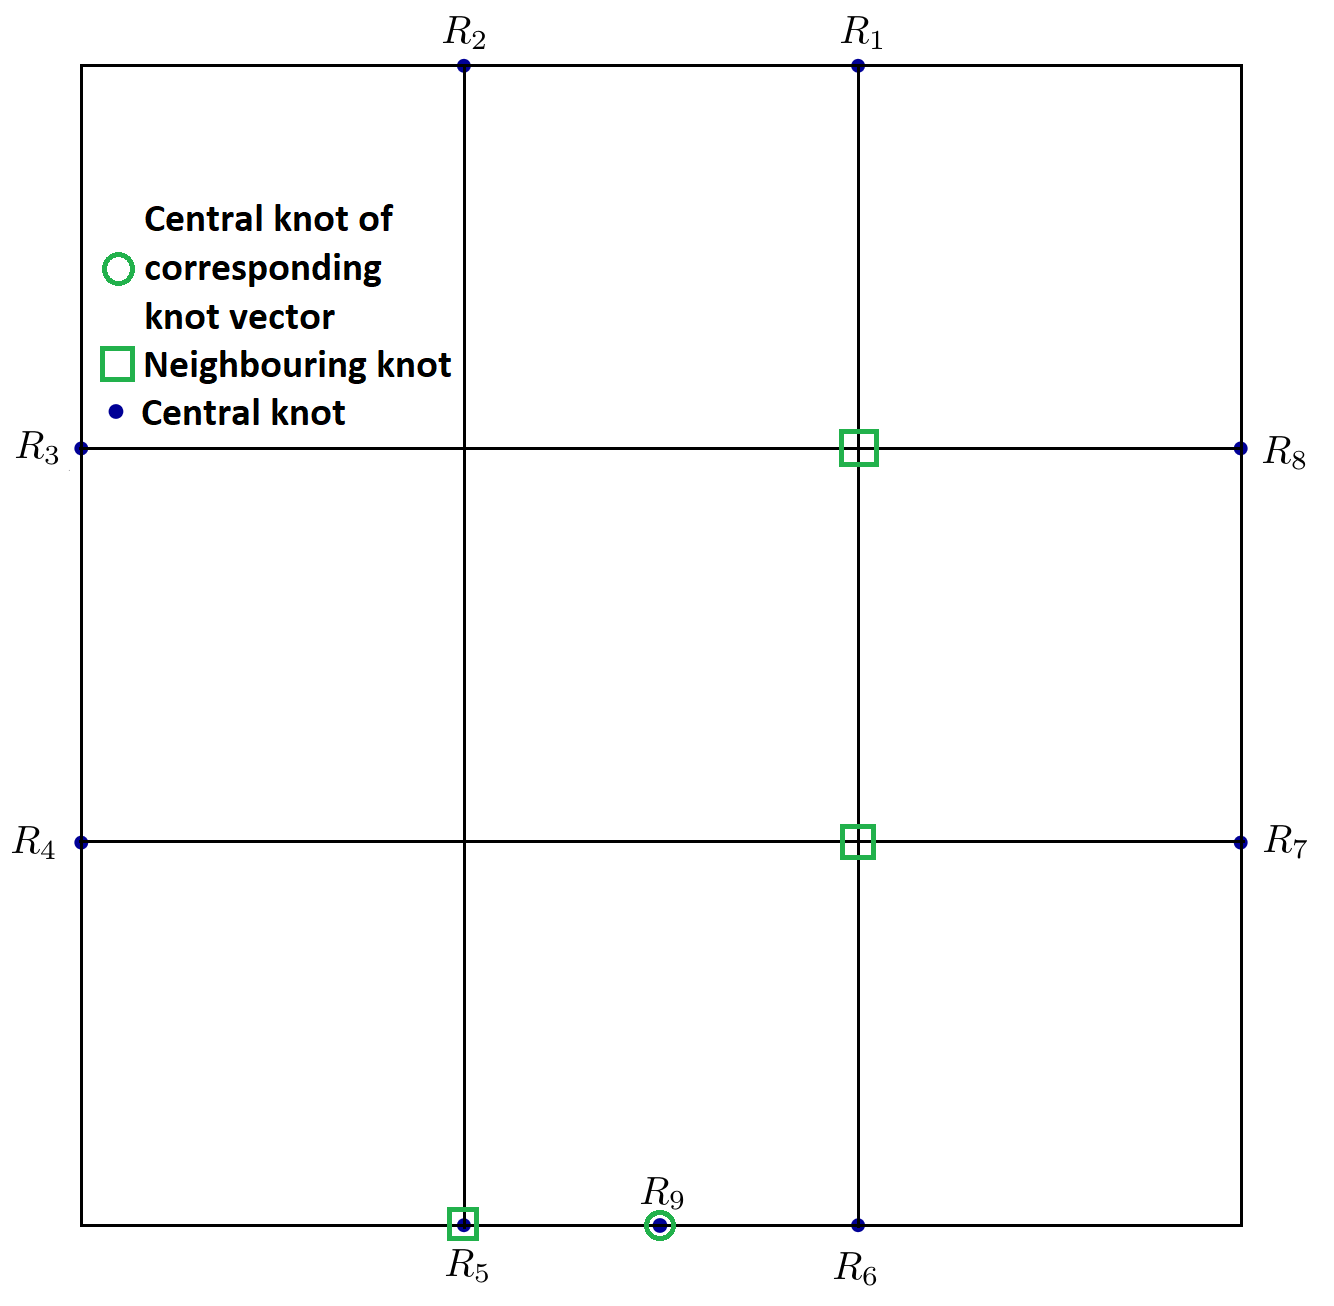
\includegraphics[width=\textwidth]{saddle5bparam}
\caption{T.}
\label{saddle5bp}
\end{subfigure}
\caption{Saddle5}
\label{saddle5p}
\end{figure}

\begin{figure}[H]
\centering
\begin{subfigure}[b]{0.48\textwidth}
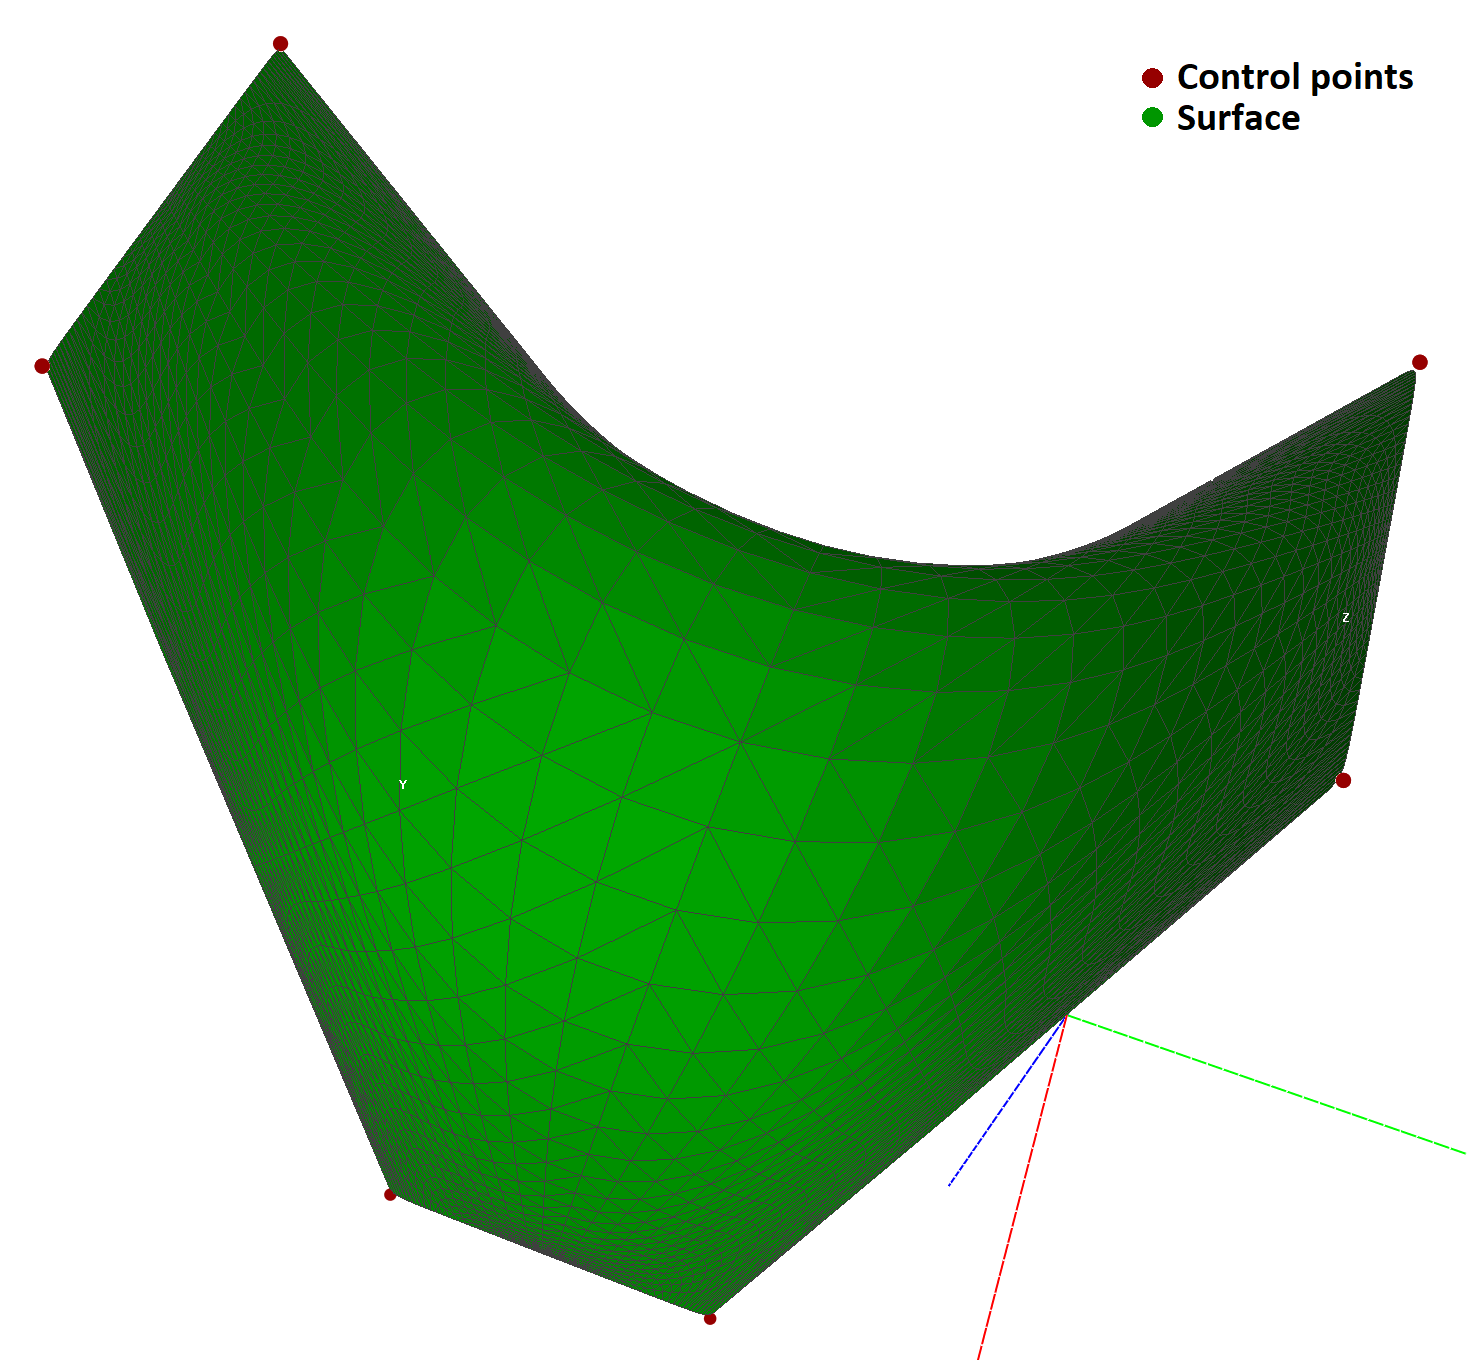
\includegraphics[width=\textwidth]{saddle5a}
\caption{Without local refinement, \texttt{saddle5a}.}
\label{saddle5a}
\end{subfigure}
\begin{subfigure}[b]{0.48\textwidth}
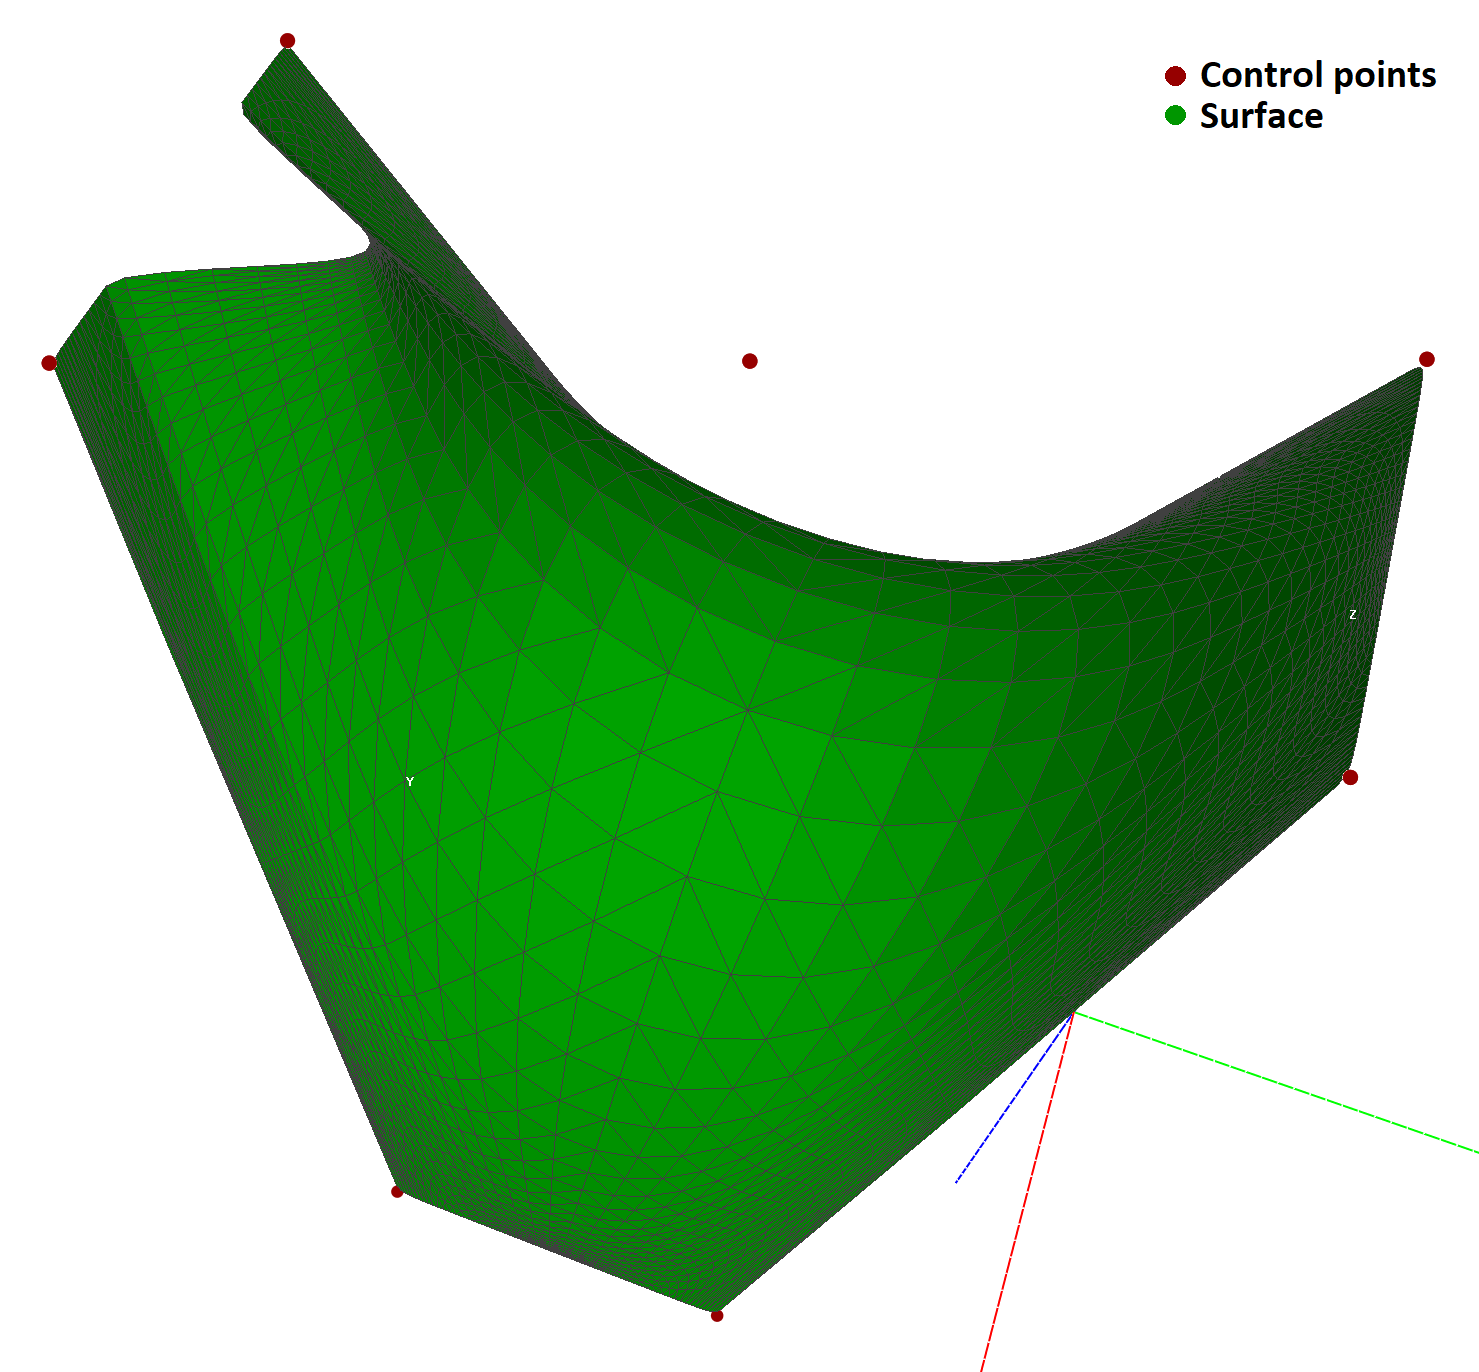
\includegraphics[width=\textwidth]{saddle5b}
\caption{With local refinement, \texttt{saddle5b}.}
\label{saddle5b}
\end{subfigure}
\caption{T-spline surfaces of \texttt{saddle5} with and without local refinement along border.}
\label{saddle5}
\end{figure}

As it was anticipated, the AOE of $R_9$ is mainly\footnote{Not entirely, because its knot vector goes until 0.67 in the perpendicular parametric direction.} visible along the border.

\subsection{$t_{i, k}$ and $t_{i, k+1}$ change}

\vspace{6pt}

In this next example, let us shift non-duplicated knots of border control points. In Figure \ref{saddle6p} one can see this specific change, and in (\ref{knotsaddle6}) the related knots.

\begin{equation}
\begin{split}
\texttt{saddle6a}: \phantom{ww} & t_{2, k. 2} = (0, 0, 0.33, 0.67, 1) \\
& t_{8, k. 1} = (0, 0.33, 0.67, 1, 1) \\
\texttt{saddle6b}: \phantom{ww} & t_{2, k. 2} = (0, 0, 0.33, 0.50, 0.67) \\
& t_{8, k. 1} = (0.33, 0.50, 0.67, 1, 1) \\
\texttt{saddle6c}: \phantom{ww} & t_{2, k. 2} = (0, 0, 0.33, 0.45, 0.55) \\
& t_{8, k. 1} = (0.45, 0.55, 0.67, 1, 1) \\
\end{split}
\label{knotsaddle6}
\end{equation}

\begin{figure}[H]
\centering
\begin{subfigure}[b]{0.32\textwidth}
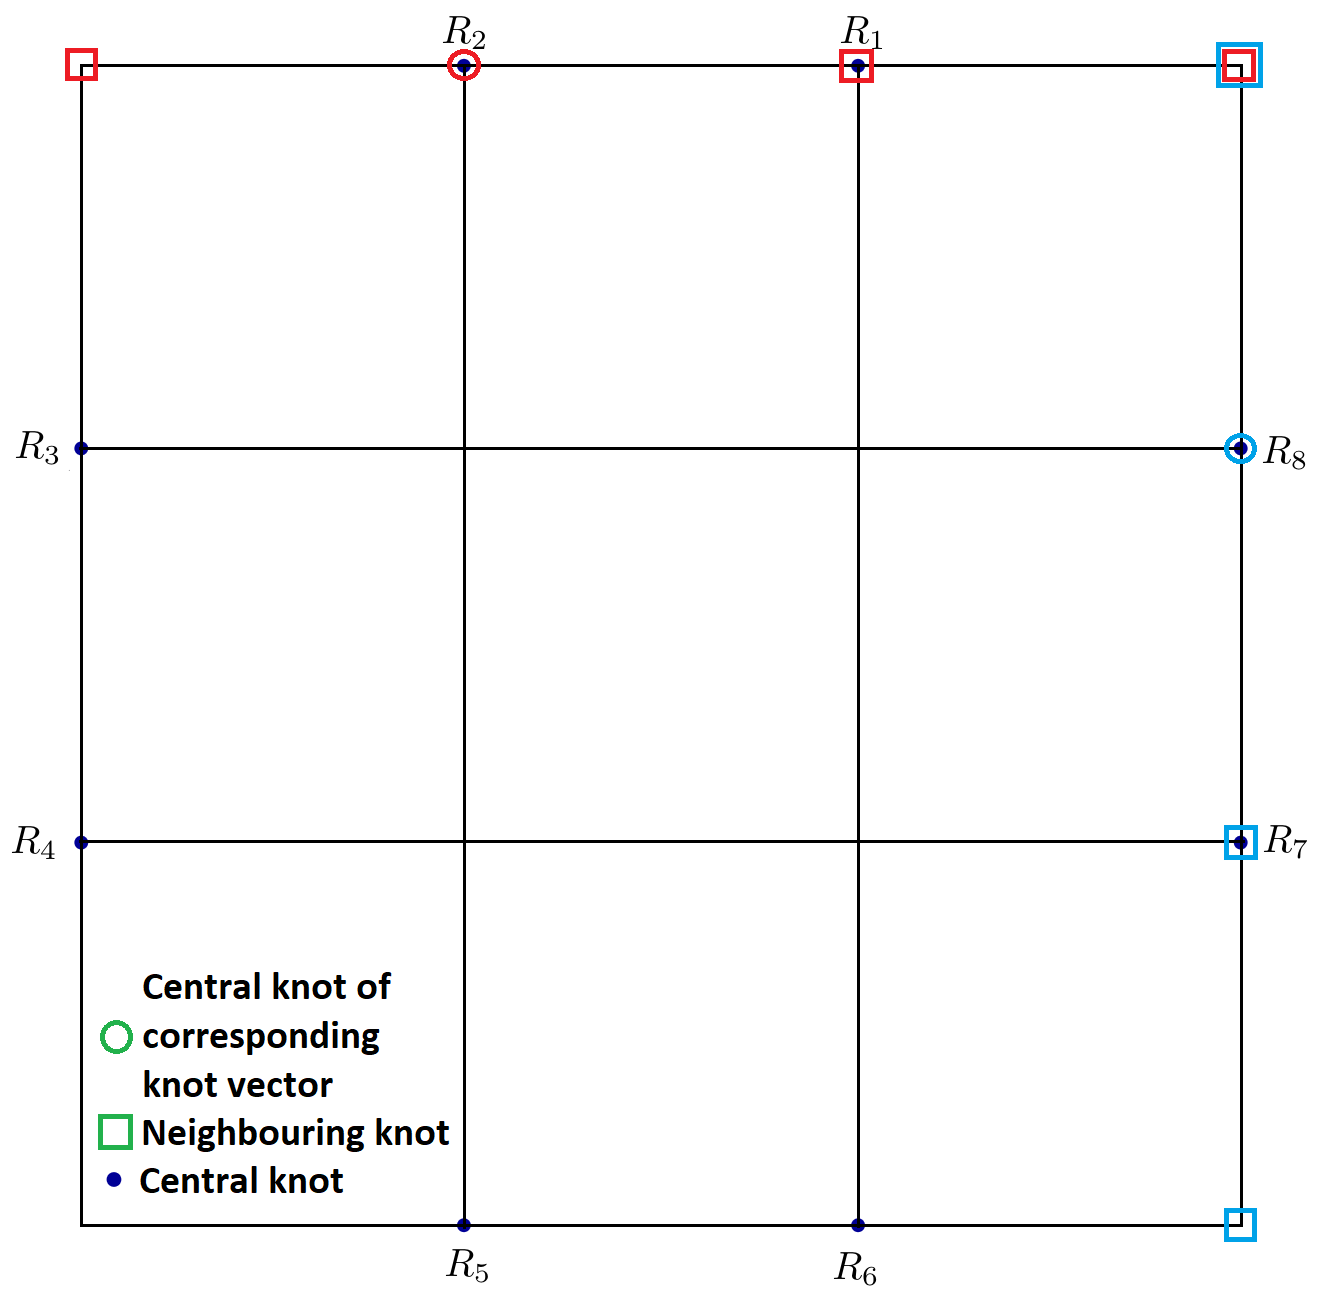
\includegraphics[width=\textwidth]{saddle6aparam}
\caption{\texttt{saddle6a}: adjacent central knots of adjacent control points along borders.}
\label{saddle6ap}
\end{subfigure}
\begin{subfigure}[b]{0.32\textwidth}
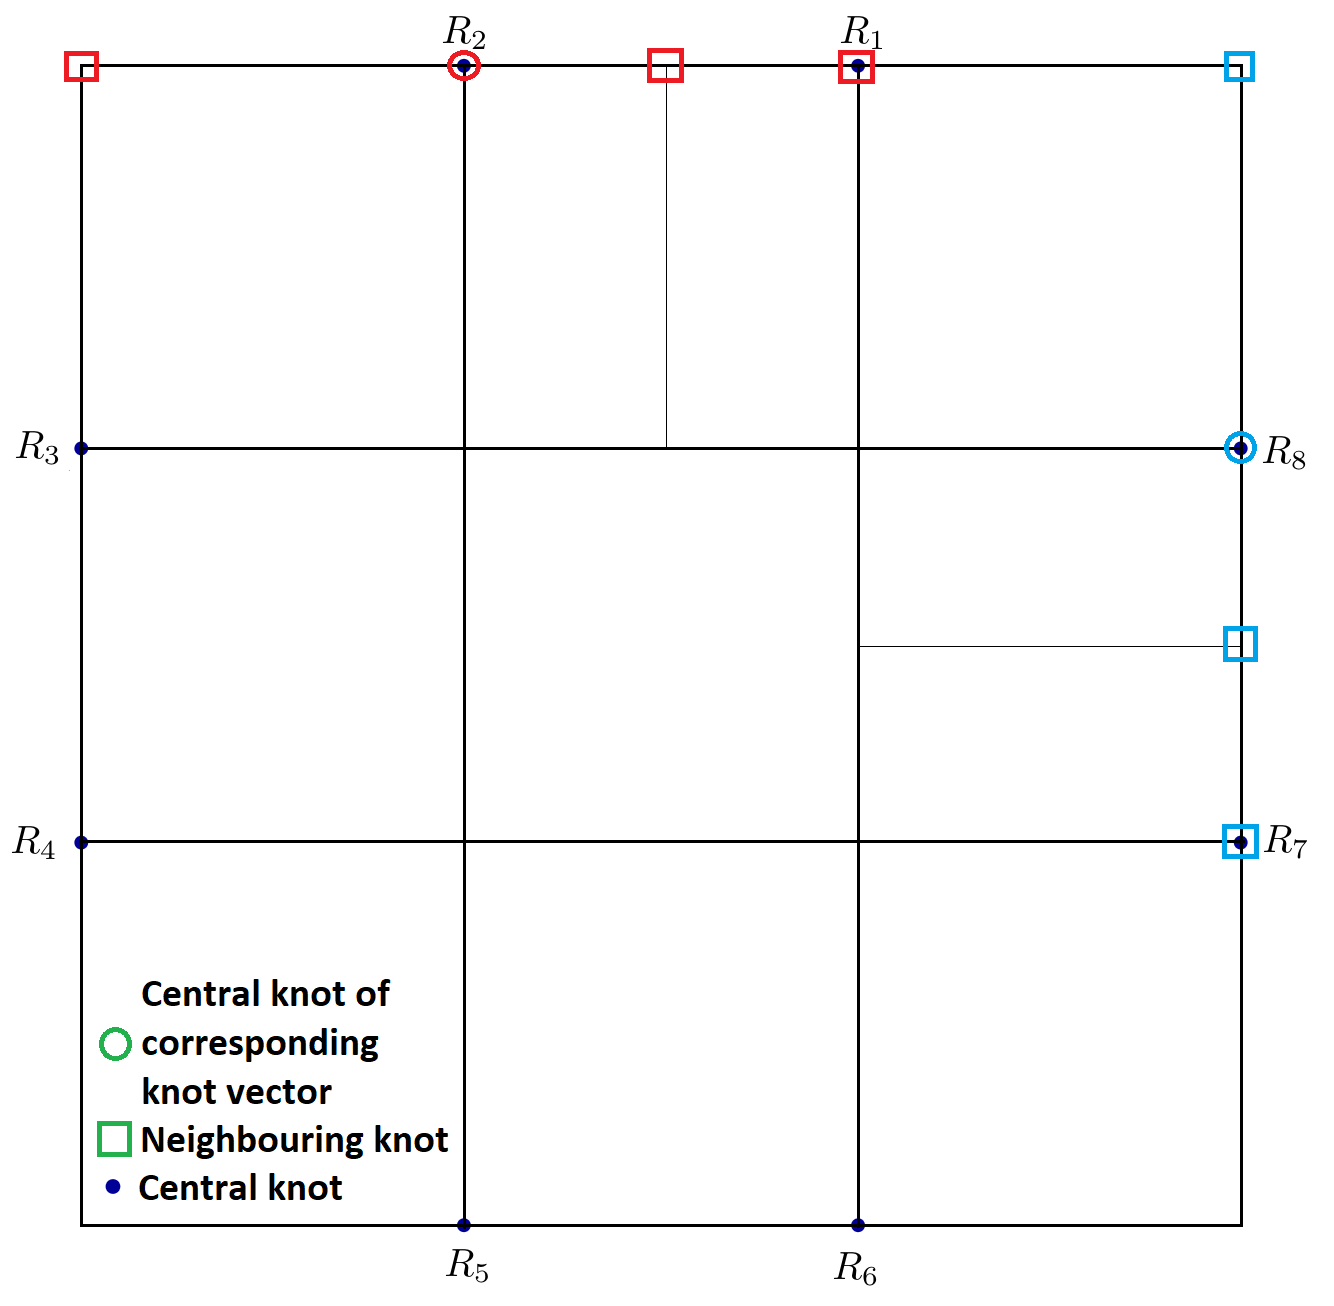
\includegraphics[width=\textwidth]{saddle6bparam}
\caption{\texttt{saddle6b}: overlapping central-adjacent knots of adjacent control points.}
\label{saddle6bp}
\end{subfigure}
\begin{subfigure}[b]{0.32\textwidth}
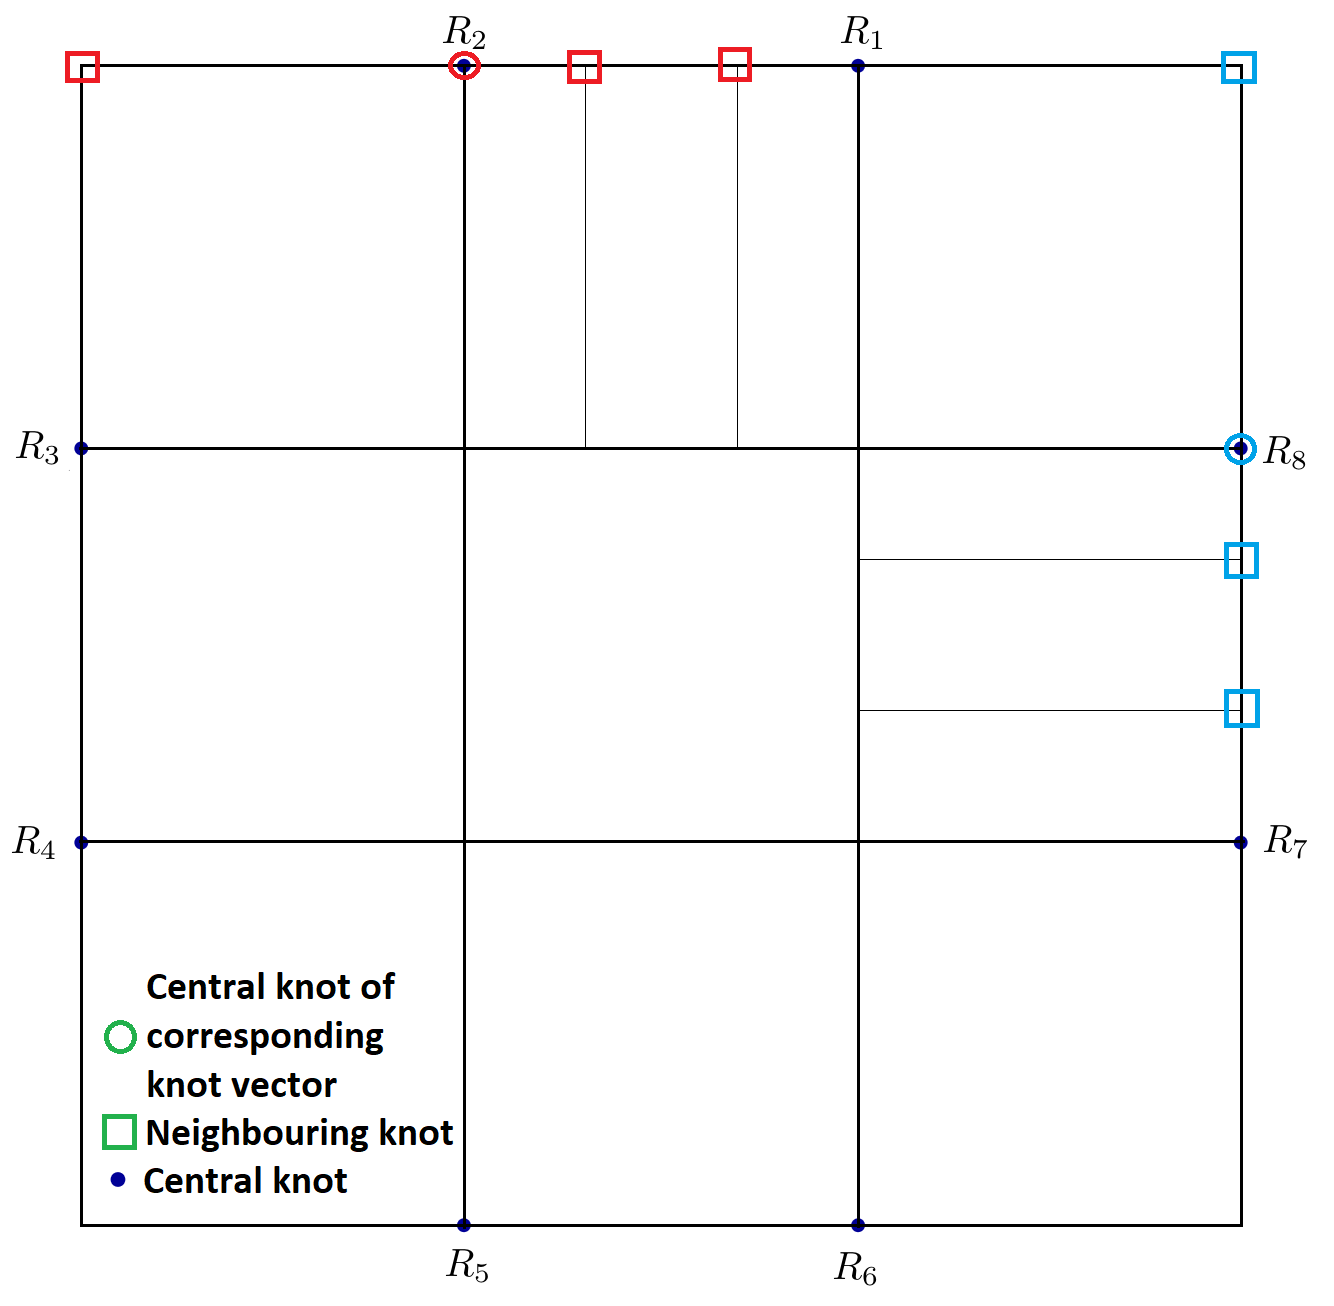
\includegraphics[width=\textwidth]{saddle6cparam}
\caption{\texttt{saddle6c}: overlapping secondary domains of adjacent control points.}
\label{saddle6cp}
\end{subfigure}
\caption{Parametric space of \texttt{saddle6}. Shifts of two knots further from corner of red and blue examples are highlighted.}
\label{saddle6p}
\end{figure}

With each shift, fewer and fewer domains overlap between adjacent control points, until no secondary knot can reach the adjacent control point's central knot. \texttt{saddle6a} is the basic setting for $R_1$, ..., $R_8$ as before. In \texttt{saddle6b} knots are already further from each other. For example $t_{2, 4, 2}$ = $t_{1, 1, 2}$, so $R_2$'s secondary domain is $R_1$'s primary domain. However, $t_{2, 4, 2}$ has no real meaning, no central knot associated with it, so the surface is expected to be less smooth, flatter as it is shown in Figure \ref{saddle6b}. The corners are more angular since the AOE of relevant control points do no reach the other end of the border.

Then another new knot is introduced between two adjacent central knots, so there are already two new knots without associated central knots. But these changes occur only along the border, in the border dimension, other remains intact. Therefore, in one dimension, we would still gain a saddle-looking shape, only in the other dimension the shape is really distorted. At this point, it gets harder and harder to predict what the surface will look like. On the other hand, it is also very questionable whether or not it makes sense to set the knots to values that are not associated with any other central knots. The reader is encouraged to try even stranger setups where adjacent control points share even fewer or no knots in the parametric space.

\begin{figure}[H]
\centering
\begin{subfigure}[b]{0.32\textwidth}
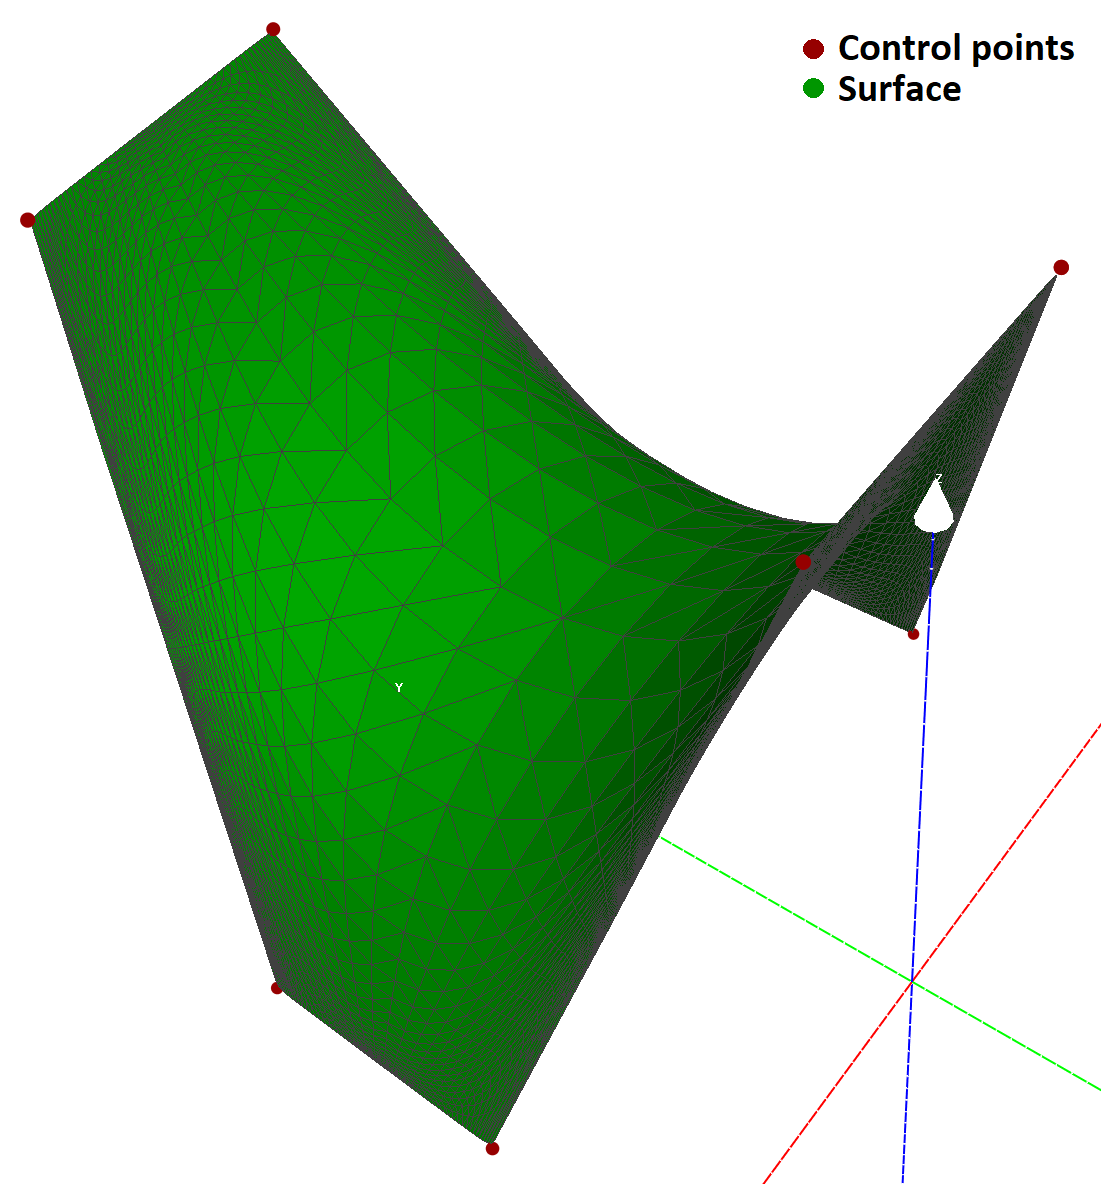
\includegraphics[width=\textwidth]{saddle6a}
\caption{Adjacent central knots.}
\label{saddle6a}
\end{subfigure}
\begin{subfigure}[b]{0.32\textwidth}
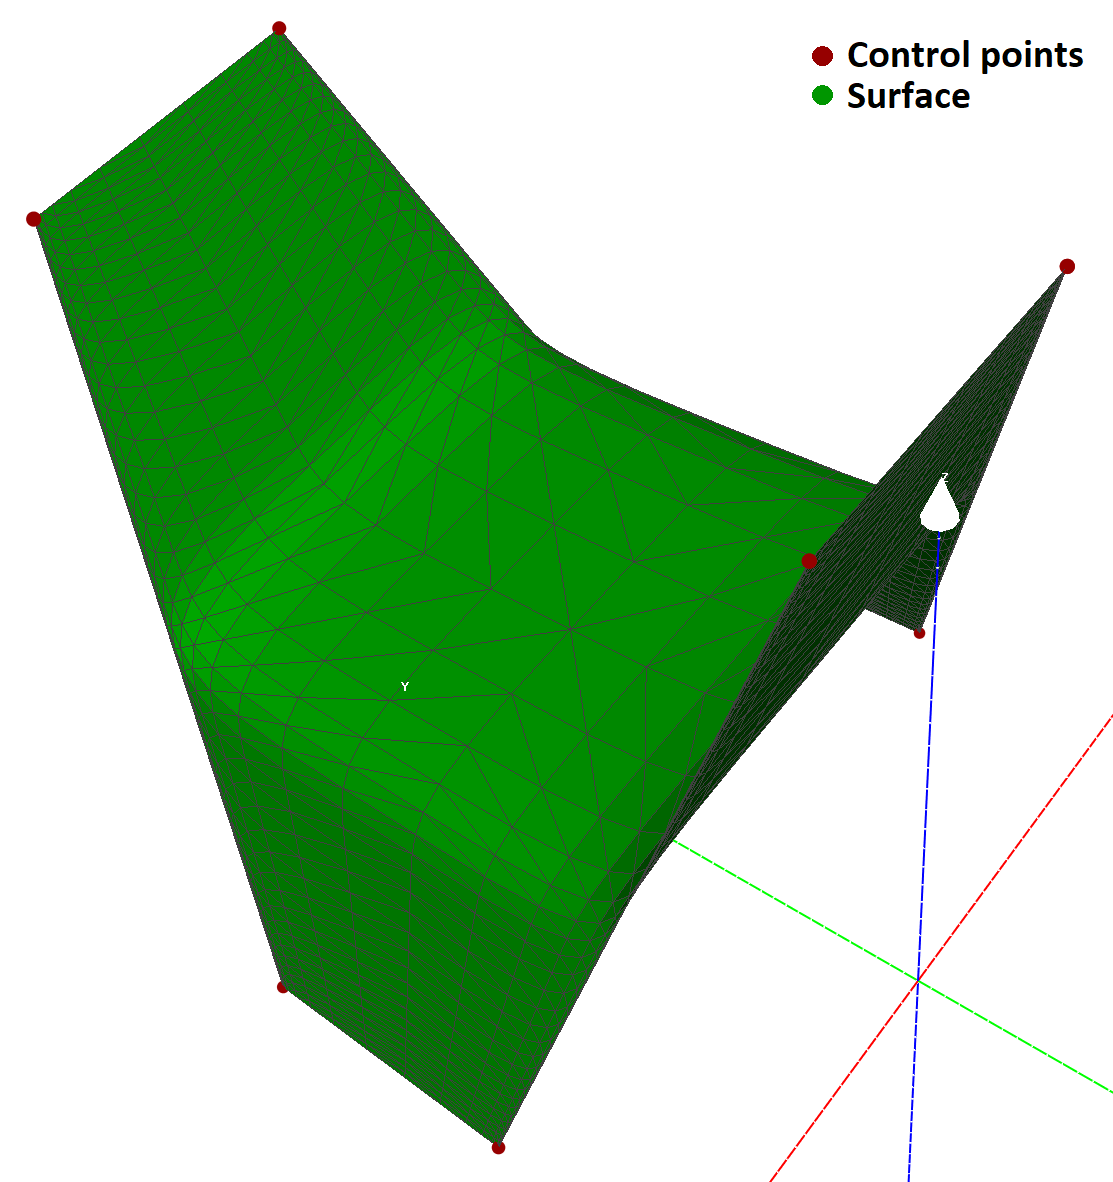
\includegraphics[width=\textwidth]{saddle6b}
\caption{Adjacent primary knots.}
\label{saddle6b}
\end{subfigure}
\begin{subfigure}[b]{0.32\textwidth}
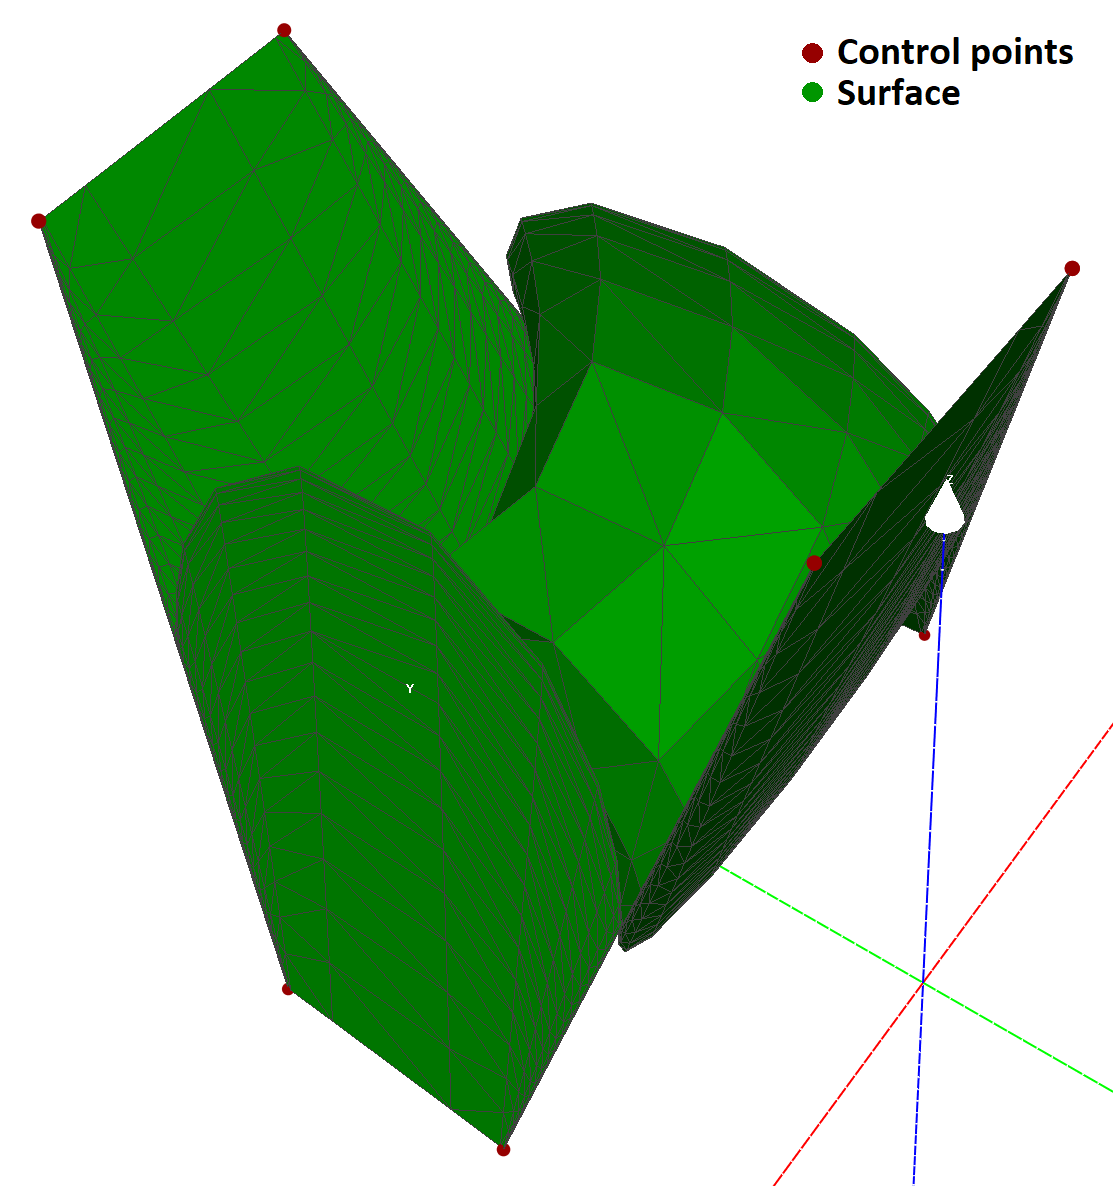
\includegraphics[width=\textwidth]{saddle6c}
\caption{Adjacent secondary knots.}
\label{saddle6c}
\end{subfigure}
\caption{T-spline surfaces of \texttt{saddle6}.}
\label{saddle6}
\end{figure}

\subsection{$T_i$ shift inside surface}

\vspace{6pt}

Let us look at the following setup: $t_{9, 1}$ and $t_{9, 5}$ are in the two corners of the parametric grid. Then $t_{9, 2}$, $t_{9, 3}$, and $t_{9, 4}$ will be shifted diagonally between those two corners as it is shown in Figure \ref{saddle7p}.

\begin{figure}[H]
\centering
\begin{subfigure}[b]{0.32\textwidth}
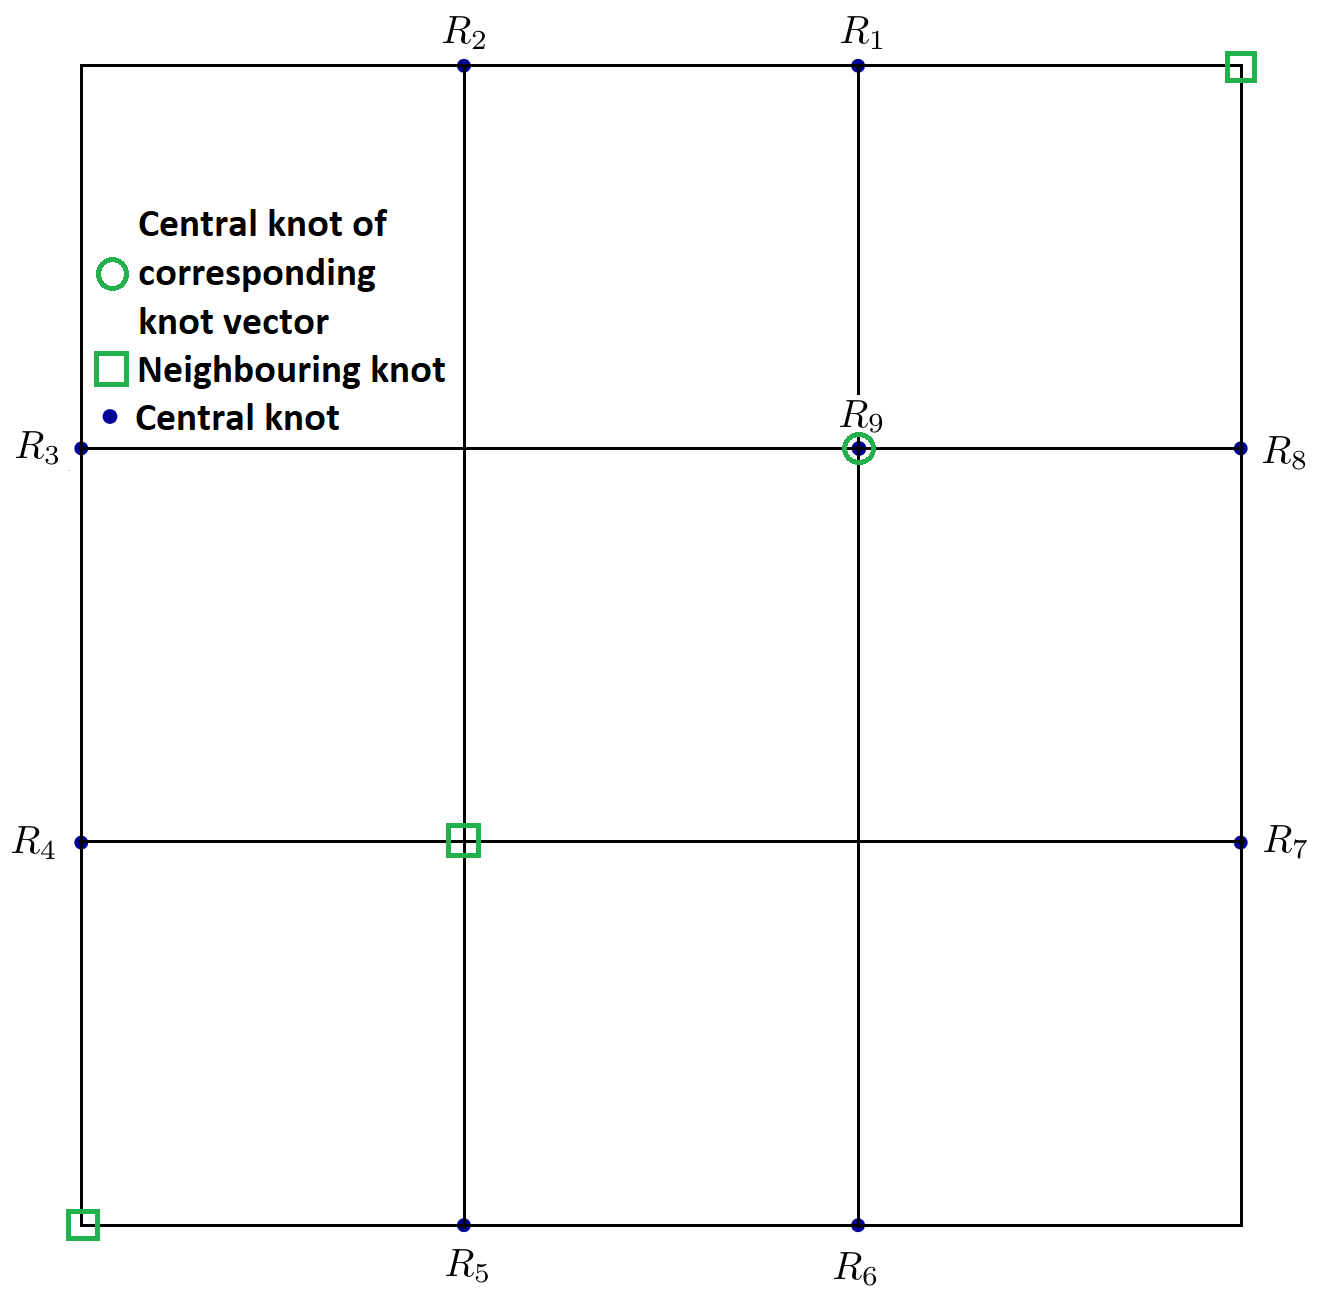
\includegraphics[width=\textwidth]{saddle7aparam}
\caption{Shift close to upper corner in \texttt{saddle7a}.}
\label{saddle7ap}
\end{subfigure}
\begin{subfigure}[b]{0.32\textwidth}
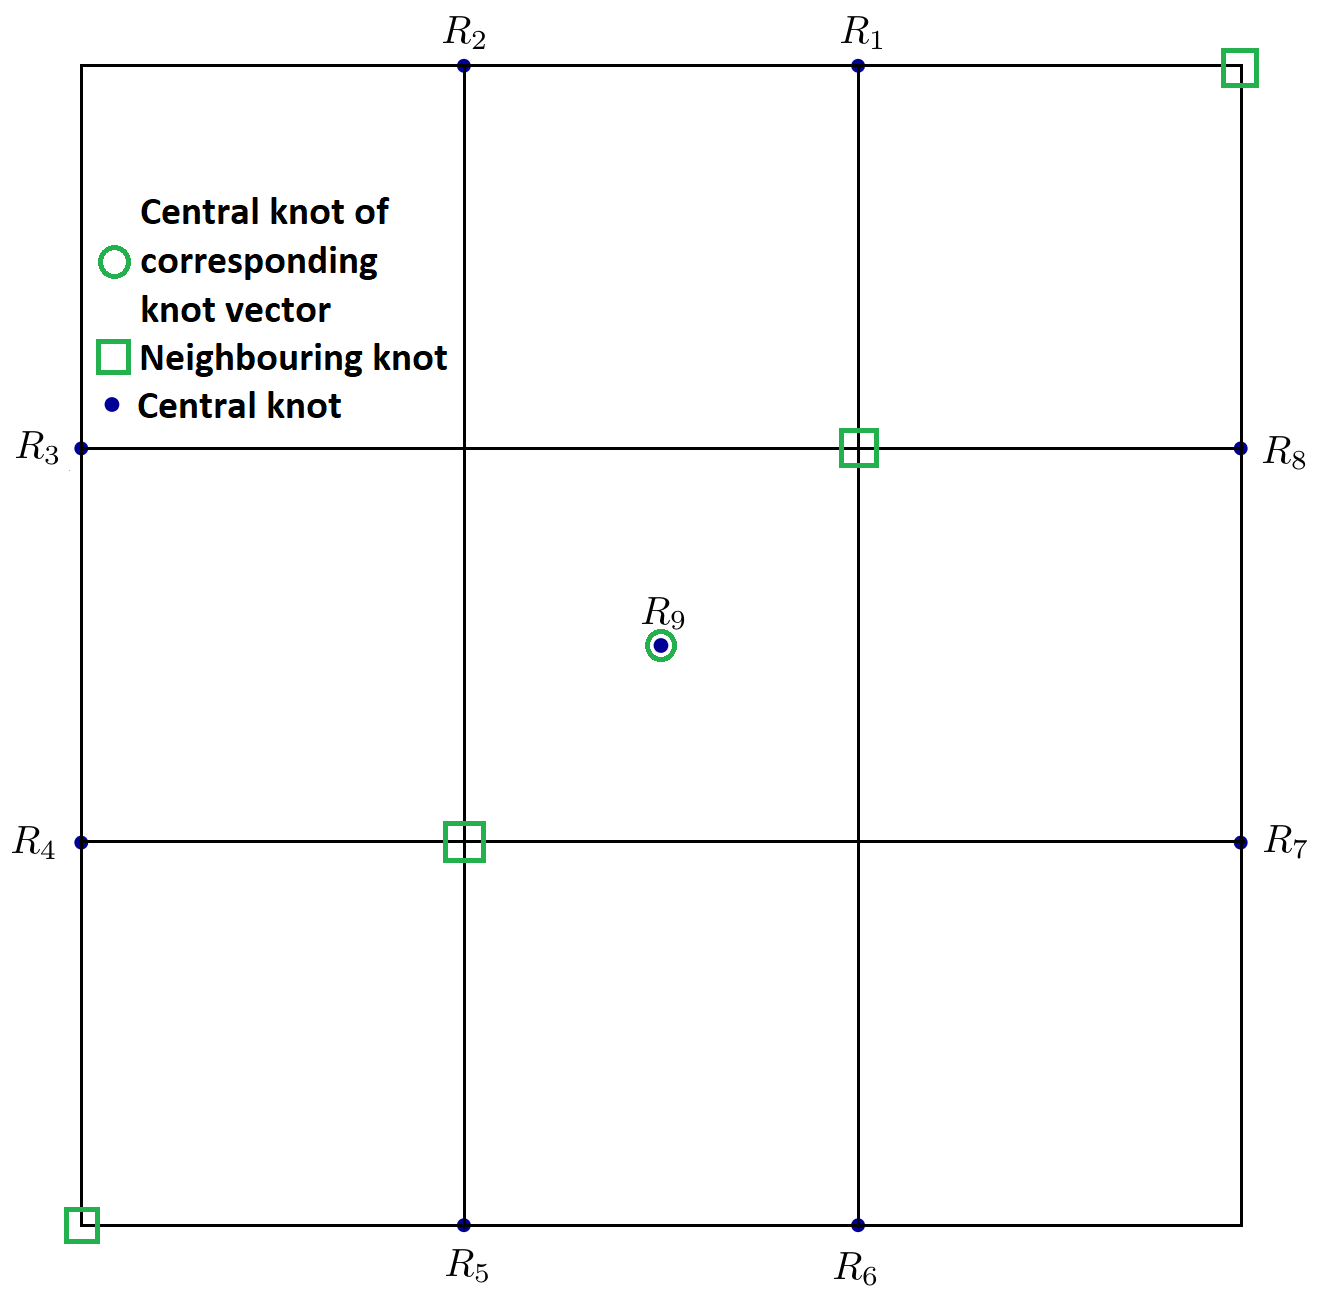
\includegraphics[width=\textwidth]{saddle7bparam}
\caption{Knots are in the middle in \texttt{saddle7b}.}
\label{saddle7bp}
\end{subfigure}
\begin{subfigure}[b]{0.32\textwidth}
\includegraphics[width=\textwidth]{saddle7cparam}
\caption{Shift close to lower corner in \texttt{saddle7c}.}
\label{saddle7cp}
\end{subfigure}
\caption{Parametric grids of \texttt{saddle7}.}
\label{saddle7p}
\end{figure}

This is in fact a local refinement in three different scenarios. The additional bump on the saddle is defined by the knots of $R_9$. Without surprise, \texttt{saddle7a} would result in a bump closer to $R_1$ and $R_8$, meanwhile in \texttt{saddle7c} the bump is closer to $R_4$ and $R_5$ as shown in Figure \ref{saddle7}. \texttt{saddle7b} is an example how to place a local bump on the surface in the middle.

\begin{figure}[H]
\centering
\begin{subfigure}[b]{0.32\textwidth}
\includegraphics[width=\textwidth]{saddle7a}
\caption{Upper bump in \texttt{saddle7a}.}
\label{saddle7a}
\end{subfigure}
\begin{subfigure}[b]{0.32\textwidth}
\includegraphics[width=\textwidth]{saddle7b}
\caption{Middle bump in \texttt{saddle7b}.}
\label{saddle7b}
\end{subfigure}
\begin{subfigure}[b]{0.32\textwidth}
\includegraphics[width=\textwidth]{saddle7c}
\caption{Lower bump in \texttt{saddle7c}.}
\label{saddle7c}
\end{subfigure}
\caption{Saddle7}
\label{saddle7}
\end{figure}

\subsection{T-spline limit goes to B-spline}

\vspace{6pt}

Last, but not least, let us demonstrate how T-spline goes to B-spline in the limit. In Figure \ref{pringle}, a Pringle is created out of 16 control points that are available in \texttt{main.go/main()}.

\begin{figure}[H]
\centering
\begin{subfigure}[b]{0.48\textwidth}
\includegraphics[width=\textwidth]{pringle_tspline}
\caption{T-spline Pringle surface.}
\label{pringlet}
\end{subfigure}
\begin{subfigure}[b]{0.48\textwidth}
\includegraphics[width=\textwidth]{pringle_bspline}
\caption{B-spline Pringle surface.}
\label{pringleb}
\end{subfigure}
\caption{Pringle surfaces made with different splines out of the same control points and knot vectors.}
\label{pringle}
\end{figure}

Every B-spline surface can be transformed to a T-spline surface without losing any information about the surface. Using the same knot vectors, same control points, the exact same surface can be created. That is why T-splines are extraordinary, because they are capable of creating the same surface, but with extra freedom of choosing costumised knot vectors, or adding local refinement.

\subsubsection{T-spline or B-spline?}

\vspace{6pt}

So if both can achieve the same, which one should we use? A big advantage of T-spline is that one can achieve the desired surface with fewer control points. That can save some computational power, which might be a bigger issue with B-splines. On the other hand, its high flexibility is also problematic when it comes to automation. In each \texttt{saddle} example, I have set up the knot vectors manually. B-spline does not require manual setup, it pairs knot vectors and control points automatically after the initial setup. That is why B-spline surfaces might be more appealing.

Local refinement cannot be achieved by B-splines. If an extra little bump is needed on a B-spline saddle, more then just one control point has to be introduced, so it would be a way more tedious work to gain the right surface. That is probably the biggest pro for T-spline surfaces.

\vspace{6pt}

There is a technique that is used to avoid the high level of complexity of T-splines, namely, the Catmull-Clark subdivision (\emph{Catmull-Clark subdivision surface}, 2022). It is used in 3D modeling softwares, such as \emph{Blender} (\emph{Catmull-Clark Subdivision Surfaces}, 2003), and it uses T-spline control points without the hassle of knot vector adjustments.


\vspace{12pt}

\begin{large}
\section{Final thoughts}
\end{large}

\vspace{12pt}

Another interesting thing that this essay did not cover is the vertex distribution on a T-spline surface. A vigilant eye might have noticed that even though equidistant values were substituted in the T-spline equations, vertices were usually not equally distributed on the surface. This is also related to the knot vectors, but due to lack of space, this essay has omitted how they could affect surface resolution.

\vspace{6pt}

With prior knowledge and some practice behind, it is possible to predict how the surface would react to different knot vectors and local refinements. The extent of a local refinement is absolutely up to the person, mathematically there are very few restrictions that have to be followed, even those can be broken technically in a code without crashing it, so it is important to pay attention to them.

This high degree of freedom of T-spline is also dangerous. If one follows the rules of B-spline, it is quite hard to go wrong, but once knot vectors are adjusted freely, it can be challenging to keep up with the transformed surface. If one wants to create a T-spline surface from scratch, my suggestion would be to start from a B-spline structure, and reduce the unnecessary control points and change the knot vectors later, once a basis form is already acceptable.

\vspace{12pt}

\begin{large}
\section{References}
\end{large}

\vspace{12pt}

$\phantom{w}$

\emph{Applications of 3D printing}. (2017, March). Wikipedia. \url{https://en.wikipedia.org/wiki/Applications_of_3D_printing}

\vspace{12pt}

Kothari, D. P., Awari, G., Shrimankar, D., $\&$ Bhende, A. (2019). \emph{Mathematics for Computer Graphics and Game Programming: A Self-Teaching Introduction}. Mercury Learning and Information.

\vspace{12pt}

Gallier, J. (2018). \emph{Curves and Surfaces In Geometric Modeling: Theory And Algorithms}. Morgan Kaufmann.

\vspace{12pt}

\emph{B-spline}. (2022, January). Wikipedia. \url{https://en.wikipedia.org/wiki/B-spline}

\vspace{12pt}

\emph{B-spline basis functions}. (2001, August). Ibiblio. \url{https://www.ibiblio.org/e-notes/Splines/basis.html}

\vspace{12pt}

\emph{B-splines}. (n. d.). University of Cambridge, Department of Computer Science and Technology. \url{https://www.cl.cam.ac.uk/teaching/1999/AGraphHCI/SMAG/node4.html}

\vspace{12pt}

\emph{B-spline curve}. (2009, December). Massachusetts Institute of Technology. \url{https://web.mit.edu/hyperbook/Patrikalakis-Maekawa-Cho/node17.html}

\vspace{12pt}

Ching-Kuang, S. (n.d.) \emph{B-spline Curves: Definition}. Michigan Technological University, Information Technology \url{https://pages.mtu.edu/~shene/COURSES/cs3621/NOTES/spline/B-spline/bspline-curve.html}

\vspace{12pt}

Sederberg, T. W., Cardon, D. L., Finnigan, G. T., North, N. S., Zheng, J., $\&$ Lyche, T. (2004). \emph{T-spline simplification and local refinement}. ACM Transactions on Graphics, 23(3), 276–283. \url{https://doi.org/10.1145/1015706.1015715}

\vspace{12pt}

Li, X., $\&$ Scott, M. A. (2014). \emph{Analysis-suitable T-splines: Characterization, refineability, and approximation}. Mathematical Models and Methods in Applied Sciences, 24(06), 1141–1164. \url{https://doi.org/10.1142/s0218202513500796}

\vspace{12pt}

Sederberg, T. W., Zheng, J., Bakenov, A., $\&$ Nasri, A. (2003). \emph{T-splines and T-NURCCs}. ACM Transactions on Graphics, 22(3), 477–484. https://doi.org/10.1145/882262.882295

\vspace{12pt}

\emph{Catmull-Clark subdivision surface}. (2022, July). Wikipedia. \url{https://en.wikipedia.org/wiki/Catmull–Clark_subdivision_surface}

\vspace{12pt}

\emph{Catmull-Clark Subdivision Surfaces}. (2003, September). Blender. \url{https://download.blender.org/documentation/html/x2615.html}

\vspace{12pt}

\begin{large}
\section{Index}
\end{large}

\vspace{12pt}

\begin{table}[H]
\centering
\begin{tabular}{L{4cm} L{10cm}}
\hline
\textbf{Area of effect} & (AOE) Surface area which a control point affects.  \\
\textbf{Central knot} & $T_3$  \\
\textbf{Domain} & Parametric space area of a control points.  \\
\textbf{Primary area of effect} & Surface area which a control point affects in the range of $T_2$-$T_3$ or $T_3$-$T_4$.  \\
\textbf{Primary domain} & Parametric space area of a control points in the range of $T_2$-$T_3$ or $T_3$-$T_4$.  \\
\textbf{Primary knot} & $T_1$ or $T_4$  \\
\textbf{Secondary area of effect} & Surface area which a control point affects in the range of $T_1$-$T_2$ or $T_4$-$T_5$.  \\
\textbf{Secondary domain} & Parametric space area of a control points in the range of $T_1$-$T_2$ or $T_4$-$T_5$.  \\
\textbf{Secondary knot} & $T_0$ or $T_5$  \\
\hline
\end{tabular}
\end{table}











\newpage


\end{document}